\section{Nonlinear Parameter Identification} 
\label{MatlabScript}

In order to carry out the parameter estimation of the water distribution, Matlab NonLinear Grey Box toolbox is used \cite{MatlabGreyBox}. This toolbox 
estimates previously defined coefficients of nonlinear differential equations, to fit with the desired data. 
Thereby, a nonlinear model has to be designed to complete the simulation. 

\subsection{NonLinear Differential Script}
\label{NLDS}
The nonlinear differential script contains all the information about the system and how it is constructed. The model needs 8 different inputs(u): 
the opening degree of the 4 PMA valves and the differential pressure across the main and PMA pumps. This inputs are obtained from the lab and are 
inserted directly into the model. Furthermore, it has been decided to include the dynamics of the system so the model remains as a nonlinear differential system. 

First, the states of the system are set. Previously in the report, the states have been defined as the chord flows and denoted as $z = [z_1 z_2 z_3 z_4 z_5 z_6 
z_7]$. The value of the states will be dependent on time, which will be specified by the data obtained from the Water Wall Setup in the lab. In this way, using
the relation stated in \eqref{ChordRelation} the flow through the edges is obtained.

The pressure across the edges has been defined in \eqref{ComponentFunction}, and in the same way has been done in Matlab. 

\begin{itemize}
  \item $\lambda$ and $\zeta$ denote the pressure in the pipes due to the friction and the elevation respectively.
  \item $\nu$ represents the pressure across the valves.
  \item $\alpha$ represent the pressure across the pumps, which is obtained from the inputs to the model.
\end{itemize}

In the system in total there are 15 pipes, the pressure across them is obtained as: 

\begin{equation}
\lambda = (C_p * abs(q)*q /(10^5*3600^2)) + ((Z)*g*1000/10^5)
\end{equation}

Where, $C_p$ denotes the friction coefficient to be estimated by the NonLinear Grey Box and $Z$ is the height of the pipes. An initial guess is done for the value of $C_p$ to minimize the error 
as possible. Moreover, the unit conversion from Bar to Pas and seconds to hours is introduced.

\begin{equation}
  Cp= f*((8*L*rho)/(pi^2*D^5))+k_f*((8*rho)/(pi^2*D^4))
\end{equation}

The $f$ and $k_f$ values are obtained as described in \eqref{turbulent} and \eqref{kfriction} with the range of values considered in \secref{FormResistance}.

In case of the valves the pressure across them is obtained as following

\begin{equation}
  mu = (1/C_v^2)* abs(q)*q /3600^2;
\end{equation}

The value of $C_v$ is obtained from the input data. When the valve is closed $\mu$ is set to 0. 

For the pumps, the pressure across them is obtained from the lab and is set as $\alpha$. 

As pointed out earlier, the inertia of the pipes is taken into account in the model and is calculated as

\begin{equation}
  J = diag((4*L*rho)/(D^2*pi*10^5*3600));
\end{equation}

Where, $L$ and $D$ are the pipes length and diameters respectively. The unit conversion is also added. 

A new matrix variable is defined containing the pressure across the edges.

\begin{equation}
  F = \lambda + \mu - \alpha
\end{equation}

The derivative of the chords can be obtained isolating $\dot{z}$ in \eqref{isolateZ}

\begin{equation}
  \dot{z}  =  - (B_1 J {B_1}^T)^{-1}B_1 F
  \label{chordder}
\end{equation}

Where, $B_1$ is the cycle matrix defined in \appref{CycleAppendix}. 

Known the derivative of the chords, the derivative of the flow through the edges is obtained

\begin{equation}
  \dot{q}  = (B_1)^T * \dot{z}
  \label{flowder}
\end{equation}

\eqref{ChordsModel} is now applied substituting $\dot{q}$ with the relations set in \eqref{flowder} and \eqref{chordder}, resulting in

\begin{equation}
  \Delta P = [(J*(B_1)^T * (B_1 J {B_1}^T)^{-1}B_1 (-\mu - \lambda + \alpha)]+\mu+\lambda-\alpha
  \label{DeltaP}
\end{equation}

Now the pressure across the edges are calculated, nevertheless, from the data of the lab the relative pressure at the nodes are obtained. This implies to 
have to calculate the pressure in the nodes so the comparison is done correctly. 

The pressure at each node can be found by applying 

\begin{equation}
  \Delta P = (H_1)^T p
\end{equation}

$\Delta P$ is known from \eqref{DeltaP}, the vector of pressure in the nodes is split up as $p = [p_o \quad p_r]$ where $p_o$ is the atmospheric pressure at 
node 1 and $p_r$ the pressure in the remaining nodes. Splitting $H_1$ matrix also

\begin{equation}
  \Delta P = [{H_o}^{T} \quad {H_r}^{T}] 
  \begin{bmatrix}
    p_o \\
    p_r
  \end{bmatrix}
\end{equation}

Isolating $p_r$ from the equation the pressure at each node is obtained

\begin{equation}
  p_r = H_r^{\dagger} (\Delta p - (H_o)^{T} p_o)
\end{equation}

$H_r^{\dagger}$ being the pseude-inverse of matrix ${H_r}^{T}$.

The outputs are set as node 2, node 4, node 5, node 7, node 10, node 11, node 15 and node 16 (see \appref{systemdiagram} for the notation). Which will be the ones that Matlab will try to fit 
to the data obtained from the setup. 

\subsection{NonLinear Grey Box Model}
The objective of using this toolbox is to obtain an estimation of the value of $C_p$ given an initial guess. For this parameters a constraint to be 
positive is set. 

The estimator compares the output. 

Several test have been done, with different inputs and outputs from the lab.


\begin{figure}[H]
\centering
\resizebox{0.75\linewidth}{!}{% This file was created by matlab2tikz.
%
%The latest updates can be retrieved from
%  http://www.mathworks.com/matlabcentral/fileexchange/22022-matlab2tikz-matlab2tikz
%where you can also make suggestions and rate matlab2tikz.
%
\definecolor{mycolor1}{rgb}{0.00000,0.44700,0.74100}%
\definecolor{mycolor2}{rgb}{0.85000,0.32500,0.09800}%
\definecolor{mycolor3}{rgb}{0.92900,0.69400,0.12500}%
\definecolor{mycolor4}{rgb}{0.49400,0.18400,0.55600}%
\definecolor{mycolor5}{rgb}{0.46600,0.67400,0.18800}%
\definecolor{mycolor6}{rgb}{0.30100,0.74500,0.93300}%
\definecolor{mycolor7}{rgb}{0.63500,0.07800,0.18400}%
%
\begin{tikzpicture}

\begin{axis}[%
width=5.511in,
height=4.471in,
at={(0.924in,0.603in)},
scale only axis,
xmin=0,
xmax=6000,
xlabel={Time samples},
ymin=0,
ymax=1,
ylabel={Pressure/Opening Degree},
axis background/.style={fill=white},
title style={font=\bfseries},
title={Input for the system},
legend style={legend cell align=left,align=left,draw=white!15!black}
]
\addplot [color=mycolor1,solid]
  table[row sep=crcr]{%
1	1\\
15	1\\
29	1\\
42	1\\
56	1\\
69	1\\
83	1\\
96	1\\
110	1\\
123	1\\
137	1\\
150	1\\
164	1\\
177	1\\
191	1\\
204	1\\
218	1\\
231	1\\
245	1\\
258	1\\
272	1\\
285	1\\
299	1\\
312	1\\
326	1\\
340	1\\
353	1\\
367	1\\
380	1\\
394	1\\
407	1\\
421	1\\
434	1\\
448	1\\
461	1\\
475	1\\
488	1\\
502	1\\
515	1\\
529	1\\
542	1\\
556	1\\
569	1\\
583	1\\
596	1\\
610	1\\
623	1\\
637	1\\
651	1\\
664	1\\
678	1\\
691	1\\
705	1\\
718	1\\
732	1\\
745	1\\
759	1\\
772	1\\
786	1\\
799	1\\
813	1\\
826	1\\
840	1\\
853	1\\
867	1\\
880	1\\
894	1\\
907	1\\
921	1\\
934	1\\
948	1\\
962	1\\
975	1\\
989	1\\
1002	1\\
1016	1\\
1029	1\\
1043	1\\
1056	1\\
1070	1\\
1083	1\\
1097	1\\
1110	1\\
1124	1\\
1137	1\\
1151	1\\
1164	1\\
1178	1\\
1191	1\\
1202	0\\
1205	0\\
1218	0\\
1232	0\\
1245	0\\
1259	0\\
1273	0\\
1286	0\\
1300	0\\
1313	0\\
1327	0\\
1340	0\\
1354	0\\
1367	0\\
1381	0\\
1394	0\\
1408	0\\
1421	0\\
1435	0\\
1448	0\\
1462	0\\
1475	0\\
1489	0\\
1502	0\\
1516	0\\
1529	0\\
1543	0\\
1556	0\\
1570	0\\
1584	0\\
1597	0\\
1611	0\\
1624	0\\
1638	0\\
1651	0\\
1665	0\\
1678	0\\
1692	0\\
1705	0\\
1719	0\\
1732	0\\
1746	0\\
1759	0\\
1773	0\\
1786	0\\
1800	0\\
1813	0\\
1827	0\\
1840	0\\
1854	0\\
1867	0\\
1881	0\\
1894	0\\
1908	0\\
1922	0\\
1935	0\\
1949	0\\
1962	0\\
1976	0\\
1989	0\\
2003	0\\
2016	0\\
2030	0\\
2043	0\\
2057	0\\
2070	0\\
2084	0\\
2097	0\\
2111	0\\
2124	0\\
2138	0\\
2151	0\\
2165	0\\
2178	0\\
2192	0\\
2205	0\\
2219	0\\
2233	0\\
2246	0\\
2260	0\\
2273	0\\
2287	0\\
2300	0\\
2314	0\\
2327	0\\
2341	0\\
2354	0\\
2368	0\\
2381	0\\
2395	0\\
2408	0\\
2422	0\\
2435	0\\
2449	0\\
2462	0\\
2476	0\\
2489	0\\
2503	0\\
2516	0\\
2530	0\\
2544	0\\
2557	0\\
2571	0\\
2584	0\\
2598	0\\
2611	0\\
2625	0\\
2638	0\\
2652	0\\
2665	0\\
2679	0\\
2692	0\\
2706	0\\
2719	0\\
2733	0\\
2746	0\\
2760	0\\
2773	0\\
2787	0\\
2800	0\\
2814	0\\
2827	0\\
2841	0\\
2855	0\\
2868	0\\
2882	0\\
2895	0\\
2909	0\\
2922	0\\
2936	0\\
2949	0\\
2963	0\\
2976	0\\
2990	0\\
3003	0\\
3017	0\\
3030	0\\
3044	0\\
3057	0\\
3071	0\\
3084	0\\
3098	0\\
3111	0\\
3125	0\\
3138	0\\
3152	0\\
3166	0\\
3179	0\\
3193	0\\
3206	0\\
3220	0\\
3233	0\\
3247	0\\
3260	0\\
3274	0\\
3287	0\\
3301	0\\
3314	0\\
3328	0\\
3341	0\\
3355	0\\
3368	0\\
3382	0\\
3395	0\\
3409	0\\
3422	0\\
3436	0\\
3449	0\\
3463	0\\
3477	0\\
3490	0\\
3504	0\\
3517	0\\
3531	0\\
3544	0\\
3558	0\\
3571	0\\
3585	0\\
3598	0\\
3612	0\\
3625	0\\
3639	0\\
3652	0\\
3666	0\\
3679	0\\
3693	0\\
3706	0\\
3720	0\\
3733	0\\
3747	0\\
3760	0\\
3774	0\\
3787	0\\
3801	0\\
3815	0\\
3828	0\\
3842	0\\
3855	0\\
3869	0\\
3882	0\\
3896	0\\
3909	0\\
3923	0\\
3936	0\\
3950	0\\
3963	0\\
3977	0\\
3990	0\\
4004	0\\
4017	0\\
4031	0\\
4044	0\\
4058	0\\
4071	0\\
4085	0\\
4098	0\\
4112	0\\
4126	0\\
4139	0\\
4153	0\\
4166	0\\
4180	0\\
4193	0\\
4207	0\\
4220	0\\
4234	0\\
4247	0\\
4261	0\\
4274	0\\
4288	0\\
4301	0\\
4315	0\\
4328	0\\
4342	0\\
4355	0\\
4369	0\\
4382	0\\
4396	0\\
4409	0\\
4423	0\\
4437	0\\
4450	0\\
4464	0\\
4477	0\\
4491	0\\
4504	0\\
4518	0\\
4531	0\\
4545	0\\
4558	0\\
4572	0\\
4585	0\\
4599	0\\
4612	0\\
4626	0\\
4639	0\\
4653	0\\
4666	0\\
4680	0\\
4693	0\\
4707	0\\
4720	0\\
4734	0\\
4748	0\\
4761	0\\
4775	0\\
4788	0\\
4802	0\\
4815	0\\
4829	0\\
4842	0\\
4856	0\\
4869	0\\
4883	0\\
4896	0\\
4910	0\\
4923	0\\
4937	0\\
4950	0\\
4964	0\\
4977	0\\
4991	0\\
5004	0\\
5018	0\\
5031	0\\
5045	0\\
5059	0\\
5072	0\\
5086	0\\
5099	0\\
5113	0\\
5126	0\\
5140	0\\
5153	0\\
5167	0\\
5180	0\\
5194	0\\
5207	0\\
5221	0\\
5234	0\\
5248	0\\
5261	0\\
5275	0\\
5288	0\\
5302	0\\
5315	0\\
5329	0\\
5342	0\\
5369	0\\
};
\addlegendentry{Valve C20 OD};

\addplot [color=mycolor2,solid]
  table[row sep=crcr]{%
1	1\\
15	1\\
29	1\\
42	1\\
56	1\\
69	1\\
83	1\\
96	1\\
110	1\\
123	1\\
137	1\\
150	1\\
164	1\\
177	1\\
191	1\\
204	1\\
218	1\\
231	1\\
245	1\\
258	1\\
272	1\\
285	1\\
299	1\\
312	1\\
326	1\\
340	1\\
353	1\\
367	1\\
380	1\\
394	1\\
407	1\\
421	1\\
434	1\\
448	1\\
461	1\\
475	1\\
488	1\\
502	1\\
515	1\\
529	1\\
542	1\\
556	1\\
569	1\\
583	1\\
596	1\\
610	1\\
623	1\\
637	1\\
651	1\\
664	1\\
678	1\\
691	1\\
705	1\\
718	1\\
732	1\\
745	1\\
759	1\\
772	1\\
786	1\\
799	1\\
813	1\\
826	1\\
840	1\\
853	1\\
867	1\\
880	1\\
894	1\\
907	1\\
921	1\\
934	1\\
948	1\\
962	1\\
975	1\\
989	1\\
1002	1\\
1016	1\\
1029	1\\
1043	1\\
1056	1\\
1070	1\\
1083	1\\
1097	1\\
1110	1\\
1124	1\\
1137	1\\
1151	1\\
1164	1\\
1178	1\\
1191	1\\
1205	1\\
1218	1\\
1232	1\\
1245	1\\
1259	1\\
1273	1\\
1286	1\\
1300	1\\
1313	1\\
1327	1\\
1340	1\\
1354	1\\
1367	1\\
1381	1\\
1394	1\\
1408	1\\
1421	1\\
1435	1\\
1448	1\\
1462	1\\
1475	1\\
1489	1\\
1502	1\\
1516	1\\
1529	1\\
1543	1\\
1556	1\\
1570	1\\
1584	1\\
1597	1\\
1611	1\\
1624	1\\
1638	1\\
1651	1\\
1665	1\\
1678	1\\
1692	1\\
1705	1\\
1719	1\\
1732	1\\
1746	1\\
1759	1\\
1773	1\\
1786	1\\
1800	1\\
1813	1\\
1827	1\\
1840	1\\
1854	1\\
1867	1\\
1881	1\\
1894	1\\
1908	1\\
1922	1\\
1935	1\\
1949	1\\
1962	1\\
1976	1\\
1989	1\\
2003	1\\
2016	1\\
2030	1\\
2043	1\\
2057	1\\
2070	1\\
2084	1\\
2097	1\\
2111	1\\
2124	1\\
2138	1\\
2151	1\\
2165	1\\
2178	1\\
2192	1\\
2205	1\\
2219	1\\
2233	1\\
2246	1\\
2260	1\\
2273	1\\
2287	1\\
2300	1\\
2314	1\\
2327	1\\
2341	1\\
2354	1\\
2368	1\\
2381	1\\
2395	1\\
2402	0\\
2408	0\\
2422	0\\
2435	0\\
2449	0\\
2462	0\\
2476	0\\
2489	0\\
2503	0\\
2516	0\\
2530	0\\
2544	0\\
2557	0\\
2571	0\\
2584	0\\
2598	0\\
2611	0\\
2625	0\\
2638	0\\
2652	0\\
2665	0\\
2679	0\\
2692	0\\
2706	0\\
2719	0\\
2733	0\\
2746	0\\
2760	0\\
2773	0\\
2787	0\\
2800	0\\
2814	0\\
2827	0\\
2841	0\\
2855	0\\
2868	0\\
2882	0\\
2895	0\\
2909	0\\
2922	0\\
2936	0\\
2949	0\\
2963	0\\
2976	0\\
2990	0\\
3003	0\\
3017	0\\
3030	0\\
3044	0\\
3057	0\\
3071	0\\
3084	0\\
3098	0\\
3111	0\\
3125	0\\
3138	0\\
3152	0\\
3166	0\\
3179	0\\
3193	0\\
3206	0\\
3220	0\\
3233	0\\
3247	0\\
3260	0\\
3274	0\\
3287	0\\
3301	0\\
3314	0\\
3328	0\\
3341	0\\
3355	0\\
3368	0\\
3382	0\\
3395	0\\
3409	0\\
3422	0\\
3436	0\\
3449	0\\
3463	0\\
3477	0\\
3490	0\\
3504	0\\
3517	0\\
3531	0\\
3544	0\\
3558	0\\
3571	0\\
3585	0\\
3598	0\\
3612	0\\
3625	0\\
3639	0\\
3652	0\\
3666	0\\
3679	0\\
3693	0\\
3706	0\\
3720	0\\
3733	0\\
3747	0\\
3760	0\\
3774	0\\
3787	0\\
3801	0\\
3815	0\\
3828	0\\
3842	0\\
3855	0\\
3869	0\\
3882	0\\
3896	0\\
3909	0\\
3923	0\\
3936	0\\
3950	0\\
3963	0\\
3977	0\\
3990	0\\
4004	0\\
4017	0\\
4031	0\\
4044	0\\
4058	0\\
4071	0\\
4085	0\\
4098	0\\
4112	0\\
4126	0\\
4139	0\\
4153	0\\
4166	0\\
4180	0\\
4193	0\\
4207	0\\
4220	0\\
4234	0\\
4247	0\\
4261	0\\
4274	0\\
4288	0\\
4301	0\\
4315	0\\
4328	0\\
4342	0\\
4355	0\\
4369	0\\
4382	0\\
4396	0\\
4409	0\\
4423	0\\
4437	0\\
4450	0\\
4464	0\\
4477	0\\
4491	0\\
4504	0\\
4518	0\\
4531	0\\
4545	0\\
4558	0\\
4572	0\\
4585	0\\
4599	0\\
4612	0\\
4626	0\\
4639	0\\
4653	0\\
4666	0\\
4680	0\\
4693	0\\
4707	0\\
4720	0\\
4734	0\\
4748	0\\
4761	0\\
4775	0\\
4788	0\\
4802	0\\
4815	0\\
4829	0\\
4842	0\\
4856	0\\
4869	0\\
4883	0\\
4896	0\\
4910	0\\
4923	0\\
4937	0\\
4950	0\\
4964	0\\
4977	0\\
4991	0\\
5004	0\\
5018	0\\
5031	0\\
5045	0\\
5059	0\\
5072	0\\
5086	0\\
5099	0\\
5113	0\\
5126	0\\
5140	0\\
5153	0\\
5167	0\\
5180	0\\
5194	0\\
5207	0\\
5221	0\\
5234	0\\
5248	0\\
5261	0\\
5275	0\\
5288	0\\
5302	0\\
5315	0\\
5329	0\\
5342	0\\
5369	0\\
};
\addlegendentry{Valve C24 OD};

\addplot [color=mycolor3,solid]
  table[row sep=crcr]{%
1	1\\
15	1\\
29	1\\
42	1\\
56	1\\
69	1\\
83	1\\
96	1\\
110	1\\
123	1\\
137	1\\
150	1\\
164	1\\
177	1\\
191	1\\
204	1\\
218	1\\
231	1\\
245	1\\
258	1\\
272	1\\
285	1\\
299	1\\
312	1\\
326	1\\
340	1\\
353	1\\
367	1\\
380	1\\
394	1\\
407	1\\
421	1\\
434	1\\
448	1\\
461	1\\
475	1\\
488	1\\
502	1\\
515	1\\
529	1\\
542	1\\
556	1\\
569	1\\
583	1\\
596	1\\
610	1\\
623	1\\
637	1\\
651	1\\
664	1\\
678	1\\
691	1\\
705	1\\
718	1\\
732	1\\
745	1\\
759	1\\
772	1\\
786	1\\
799	1\\
813	1\\
826	1\\
840	1\\
853	1\\
867	1\\
880	1\\
894	1\\
907	1\\
921	1\\
934	1\\
948	1\\
962	1\\
975	1\\
989	1\\
1002	1\\
1016	1\\
1029	1\\
1043	1\\
1056	1\\
1070	1\\
1083	1\\
1097	1\\
1110	1\\
1124	1\\
1137	1\\
1151	1\\
1164	1\\
1178	1\\
1191	1\\
1205	1\\
1218	1\\
1232	1\\
1245	1\\
1259	1\\
1273	1\\
1286	1\\
1300	1\\
1313	1\\
1327	1\\
1340	1\\
1354	1\\
1367	1\\
1381	1\\
1394	1\\
1408	1\\
1421	1\\
1435	1\\
1448	1\\
1462	1\\
1475	1\\
1489	1\\
1502	1\\
1516	1\\
1529	1\\
1543	1\\
1556	1\\
1570	1\\
1584	1\\
1597	1\\
1611	1\\
1624	1\\
1638	1\\
1651	1\\
1665	1\\
1678	1\\
1692	1\\
1705	1\\
1719	1\\
1732	1\\
1746	1\\
1759	1\\
1773	1\\
1786	1\\
1800	1\\
1813	1\\
1827	1\\
1840	1\\
1854	1\\
1867	1\\
1881	1\\
1894	1\\
1908	1\\
1922	1\\
1935	1\\
1949	1\\
1962	1\\
1976	1\\
1989	1\\
2003	1\\
2016	1\\
2030	1\\
2043	1\\
2057	1\\
2070	1\\
2084	1\\
2097	1\\
2111	1\\
2124	1\\
2138	1\\
2151	1\\
2165	1\\
2178	1\\
2192	1\\
2205	1\\
2219	1\\
2233	1\\
2246	1\\
2260	1\\
2273	1\\
2287	1\\
2300	1\\
2314	1\\
2327	1\\
2341	1\\
2354	1\\
2368	1\\
2381	1\\
2395	1\\
2408	1\\
2422	1\\
2435	1\\
2449	1\\
2462	1\\
2476	1\\
2489	1\\
2503	1\\
2516	1\\
2530	1\\
2544	1\\
2557	1\\
2571	1\\
2584	1\\
2598	1\\
2611	1\\
2625	1\\
2638	1\\
2652	1\\
2665	1\\
2679	1\\
2692	1\\
2706	1\\
2719	1\\
2733	1\\
2746	1\\
2760	1\\
2773	1\\
2787	1\\
2800	1\\
2814	1\\
2827	1\\
2841	1\\
2855	1\\
2868	1\\
2882	1\\
2895	1\\
2909	1\\
2922	1\\
2936	1\\
2949	1\\
2963	1\\
2976	1\\
2990	1\\
3003	1\\
3017	1\\
3030	1\\
3044	1\\
3057	1\\
3071	1\\
3084	1\\
3098	1\\
3111	1\\
3125	1\\
3138	1\\
3152	1\\
3166	1\\
3179	1\\
3193	1\\
3206	1\\
3220	1\\
3233	1\\
3247	1\\
3260	1\\
3274	1\\
3287	1\\
3301	1\\
3314	1\\
3328	1\\
3341	1\\
3355	1\\
3368	1\\
3382	1\\
3395	1\\
3409	1\\
3422	1\\
3436	1\\
3449	1\\
3463	1\\
3477	1\\
3490	1\\
3504	1\\
3517	1\\
3531	1\\
3544	1\\
3558	1\\
3571	1\\
3585	1\\
3598	1\\
3602	0\\
3612	0\\
3625	0\\
3639	0\\
3652	0\\
3666	0\\
3679	0\\
3693	0\\
3706	0\\
3720	0\\
3733	0\\
3747	0\\
3760	0\\
3774	0\\
3787	0\\
3801	0\\
3815	0\\
3828	0\\
3842	0\\
3855	0\\
3869	0\\
3882	0\\
3896	0\\
3909	0\\
3923	0\\
3936	0\\
3950	0\\
3963	0\\
3977	0\\
3990	0\\
4004	0\\
4017	0\\
4031	0\\
4044	0\\
4058	0\\
4071	0\\
4085	0\\
4098	0\\
4112	0\\
4126	0\\
4139	0\\
4153	0\\
4166	0\\
4180	0\\
4193	0\\
4207	0\\
4220	0\\
4234	0\\
4247	0\\
4261	0\\
4274	0\\
4288	0\\
4301	0\\
4315	0\\
4328	0\\
4342	0\\
4355	0\\
4369	0\\
4382	0\\
4396	0\\
4409	0\\
4423	0\\
4437	0\\
4450	0\\
4464	0\\
4477	0\\
4491	0\\
4504	0\\
4518	0\\
4531	0\\
4545	0\\
4558	0\\
4572	0\\
4585	0\\
4599	0\\
4612	0\\
4626	0\\
4639	0\\
4653	0\\
4666	0\\
4680	0\\
4693	0\\
4707	0\\
4720	0\\
4734	0\\
4748	0\\
4761	0\\
4775	0\\
4788	0\\
4802	0\\
4815	0\\
4829	0\\
4842	0\\
4856	0\\
4869	0\\
4883	0\\
4896	0\\
4910	0\\
4923	0\\
4937	0\\
4950	0\\
4964	0\\
4977	0\\
4991	0\\
5004	0\\
5018	0\\
5031	0\\
5045	0\\
5059	0\\
5072	0\\
5086	0\\
5099	0\\
5113	0\\
5126	0\\
5140	0\\
5153	0\\
5167	0\\
5180	0\\
5194	0\\
5207	0\\
5221	0\\
5234	0\\
5248	0\\
5261	0\\
5275	0\\
5288	0\\
5302	0\\
5315	0\\
5329	0\\
5342	0\\
5369	0\\
};
\addlegendentry{Valve C27 OD};

\addplot [color=mycolor4,solid]
  table[row sep=crcr]{%
1	1\\
15	1\\
29	1\\
42	1\\
56	1\\
69	1\\
83	1\\
96	1\\
110	1\\
123	1\\
137	1\\
150	1\\
164	1\\
177	1\\
191	1\\
204	1\\
218	1\\
231	1\\
245	1\\
258	1\\
272	1\\
285	1\\
299	1\\
312	1\\
326	1\\
340	1\\
353	1\\
367	1\\
380	1\\
394	1\\
407	1\\
421	1\\
434	1\\
448	1\\
461	1\\
475	1\\
488	1\\
502	1\\
515	1\\
529	1\\
542	1\\
556	1\\
569	1\\
583	1\\
596	1\\
610	1\\
623	1\\
637	1\\
651	1\\
664	1\\
678	1\\
691	1\\
705	1\\
718	1\\
732	1\\
745	1\\
759	1\\
772	1\\
786	1\\
799	1\\
813	1\\
826	1\\
840	1\\
853	1\\
867	1\\
880	1\\
894	1\\
907	1\\
921	1\\
934	1\\
948	1\\
962	1\\
975	1\\
989	1\\
1002	1\\
1016	1\\
1029	1\\
1043	1\\
1056	1\\
1070	1\\
1083	1\\
1097	1\\
1110	1\\
1124	1\\
1137	1\\
1151	1\\
1164	1\\
1178	1\\
1191	1\\
1205	1\\
1218	1\\
1232	1\\
1245	1\\
1259	1\\
1273	1\\
1286	1\\
1300	1\\
1313	1\\
1327	1\\
1340	1\\
1354	1\\
1367	1\\
1381	1\\
1394	1\\
1408	1\\
1421	1\\
1435	1\\
1448	1\\
1462	1\\
1475	1\\
1489	1\\
1502	1\\
1516	1\\
1529	1\\
1543	1\\
1556	1\\
1570	1\\
1584	1\\
1597	1\\
1611	1\\
1624	1\\
1638	1\\
1651	1\\
1665	1\\
1678	1\\
1692	1\\
1705	1\\
1719	1\\
1732	1\\
1746	1\\
1759	1\\
1773	1\\
1786	1\\
1800	1\\
1813	1\\
1827	1\\
1840	1\\
1854	1\\
1867	1\\
1881	1\\
1894	1\\
1908	1\\
1922	1\\
1935	1\\
1949	1\\
1962	1\\
1976	1\\
1989	1\\
2003	1\\
2016	1\\
2030	1\\
2043	1\\
2057	1\\
2070	1\\
2084	1\\
2097	1\\
2111	1\\
2124	1\\
2138	1\\
2151	1\\
2165	1\\
2178	1\\
2192	1\\
2205	1\\
2219	1\\
2233	1\\
2246	1\\
2260	1\\
2273	1\\
2287	1\\
2300	1\\
2314	1\\
2327	1\\
2341	1\\
2354	1\\
2368	1\\
2381	1\\
2395	1\\
2408	1\\
2422	1\\
2435	1\\
2449	1\\
2462	1\\
2476	1\\
2489	1\\
2503	1\\
2516	1\\
2530	1\\
2544	1\\
2557	1\\
2571	1\\
2584	1\\
2598	1\\
2611	1\\
2625	1\\
2638	1\\
2652	1\\
2665	1\\
2679	1\\
2692	1\\
2706	1\\
2719	1\\
2733	1\\
2746	1\\
2760	1\\
2773	1\\
2787	1\\
2800	1\\
2814	1\\
2827	1\\
2841	1\\
2855	1\\
2868	1\\
2882	1\\
2895	1\\
2909	1\\
2922	1\\
2936	1\\
2949	1\\
2963	1\\
2976	1\\
2990	1\\
3003	1\\
3017	1\\
3030	1\\
3044	1\\
3057	1\\
3071	1\\
3084	1\\
3098	1\\
3111	1\\
3125	1\\
3138	1\\
3152	1\\
3166	1\\
3179	1\\
3193	1\\
3206	1\\
3220	1\\
3233	1\\
3247	1\\
3260	1\\
3274	1\\
3287	1\\
3301	1\\
3314	1\\
3328	1\\
3341	1\\
3355	1\\
3368	1\\
3382	1\\
3395	1\\
3409	1\\
3422	1\\
3436	1\\
3449	1\\
3463	1\\
3477	1\\
3490	1\\
3504	1\\
3517	1\\
3531	1\\
3544	1\\
3558	1\\
3571	1\\
3585	1\\
3598	1\\
3612	1\\
3625	1\\
3639	1\\
3652	1\\
3666	1\\
3679	1\\
3693	1\\
3706	1\\
3720	1\\
3733	1\\
3747	1\\
3760	1\\
3774	1\\
3787	1\\
3801	1\\
3815	1\\
3828	1\\
3842	1\\
3855	1\\
3869	1\\
3882	1\\
3896	1\\
3909	1\\
3923	1\\
3936	1\\
3950	1\\
3963	1\\
3977	1\\
3990	1\\
4004	1\\
4017	1\\
4031	1\\
4044	1\\
4058	1\\
4071	1\\
4085	1\\
4098	1\\
4112	1\\
4126	1\\
4139	1\\
4153	1\\
4166	1\\
4180	1\\
4193	1\\
4207	1\\
4220	1\\
4234	1\\
4247	1\\
4261	1\\
4274	1\\
4288	1\\
4301	1\\
4315	1\\
4328	1\\
4342	1\\
4355	1\\
4369	1\\
4382	1\\
4396	1\\
4409	1\\
4423	1\\
4437	1\\
4450	1\\
4464	1\\
4477	1\\
4491	1\\
4504	1\\
4518	1\\
4531	1\\
4545	1\\
4558	1\\
4572	1\\
4585	1\\
4599	1\\
4612	1\\
4626	1\\
4639	1\\
4653	1\\
4666	1\\
4680	1\\
4693	1\\
4707	1\\
4720	1\\
4734	1\\
4748	1\\
4761	1\\
4775	1\\
4788	1\\
4802	0\\
4815	0\\
4829	0\\
4842	0\\
4856	0\\
4869	0\\
4883	0\\
4896	0\\
4910	0\\
4923	0\\
4937	0\\
4950	0\\
4964	0\\
4977	0\\
4991	0\\
5004	0\\
5018	0\\
5031	0\\
5045	0\\
5059	0\\
5072	0\\
5086	0\\
5099	0\\
5113	0\\
5126	0\\
5140	0\\
5153	0\\
5167	0\\
5180	0\\
5194	0\\
5207	0\\
5221	0\\
5234	0\\
5248	0\\
5261	0\\
5275	0\\
5288	0\\
5302	0\\
5315	0\\
5329	0\\
5342	0\\
5369	0\\
};
\addlegendentry{Valve C31 OD};

\addplot [color=mycolor5,solid]
  table[row sep=crcr]{%
1	0\\
15	0\\
29	0\\
42	0\\
56	0\\
69	0\\
83	0\\
96	0\\
110	0.390255376344086\\
123	0.455101417399805\\
137	0.487176197458455\\
150	0.49005376344086\\
164	0.493169599217986\\
177	0.497214076246334\\
191	0.500213831867056\\
204	0.502413245356792\\
218	0.505718475073312\\
231	0.508687683284455\\
243	0.509255865102637\\
251	0.509200879765394\\
257	0.509329178885628\\
258	0.509316959921796\\
267	0.509182551319646\\
272	0.509304740957965\\
284	0.508962609970673\\
285	0.509023704789832\\
298	0.50989736070381\\
299	0.509872922776147\\
307	0.509707966764417\\
312	0.50979349951124\\
326	0.509426930596284\\
329	0.509310850439881\\
338	0.50946358748778\\
340	0.509359726295209\\
348	0.509127565982403\\
353	0.509127565982404\\
364	0.508956500488758\\
367	0.509054252199414\\
372	0.508901515151517\\
380	0.508999266862174\\
394	0.508822091886613\\
402	0.509048142717505\\
415	0.508748778103623\\
421	0.508938172043018\\
423	0.508925953079187\\
430	0.509060361681339\\
434	0.509042033235591\\
446	0.508962609970684\\
448	0.508993157380265\\
461	0.50907869012709\\
465	0.509103128054754\\
473	0.508962609970684\\
475	0.5089687194526\\
488	0.509103128054752\\
497	0.5091214565005\\
502	0.508962609970684\\
515	0.509261974584569\\
516	0.509274193548401\\
529	0.509023704789845\\
533	0.509054252199426\\
539	0.508938172043021\\
542	0.509048142717509\\
548	0.509133675464334\\
557	0.509097018572838\\
569	0.508956500488771\\
583	0.508760997067459\\
596	0.50855938416423\\
598	0.50849828934507\\
603	0.508675464320634\\
616	0.50868157380255\\
622	0.508559384164229\\
630	0.508620478983388\\
634	0.508455522971656\\
639	0.508620478983388\\
651	0.50844941348974\\
652	0.508443304007824\\
662	0.508596041055723\\
665	0.508547165200395\\
671	0.508706011730208\\
679	0.508693792766373\\
689	0.508840420332352\\
698	0.508877077223845\\
705	0.508693792766362\\
711	0.508724340175939\\
716	0.508510508308878\\
718	0.508608260019533\\
732	0.508858748778082\\
734	0.508919843597242\\
739	0.508797653958921\\
746	0.508809872922748\\
752	0.509023704789804\\
761	0.508803763440825\\
772	0.50897482893447\\
774	0.509011485825965\\
784	0.508852639296151\\
789	0.508815982404656\\
793	0.508950391006806\\
807	0.509017595307881\\
811	0.508846529814235\\
815	0.50897482893447\\
825	0.508681573802505\\
834	0.508675464320589\\
840	0.50877932551316\\
847	0.508883186705731\\
852	0.508693792766337\\
857	0.508663245356757\\
864	0.508791544476992\\
870	0.508724340175917\\
880	0.508901515151479\\
889	0.509103128054704\\
894	0.508980938416386\\
903	0.509206989247275\\
907	0.509206989247275\\
920	0.509384164222837\\
921	0.509371945259005\\
933	0.50943914956008\\
934	0.509433040078164\\
941	0.509347507331341\\
948	0.509378054740921\\
956	0.509292521994098\\
962	0.509353616813257\\
975	0.509188660801527\\
979	0.509072580645125\\
993	0.50927419354835\\
1002	0.508993157380218\\
1016	0.509280303030266\\
1023	0.50933528836751\\
1029	0.509237536656855\\
1037	0.509310850439846\\
1043	0.509121456500452\\
1045	0.509084799608956\\
1056	0.509310850439846\\
1070	0.509445259041996\\
1074	0.509433040078164\\
1079	0.509518572824987\\
1083	0.509481915933492\\
1097	0.509231427174939\\
1101	0.509353616813257\\
1110	0.509127565982368\\
1124	0.508846529814235\\
1135	0.50897482893447\\
1137	0.508925953079142\\
1143	0.509097018572788\\
1156	0.509121456500452\\
1164	0.50894428152489\\
1175	0.509054252199377\\
1178	0.509048142717461\\
1187	0.508919843597226\\
1196	0.509035923753629\\
1205	0.508950391006806\\
1218	0.505516862170055\\
1232	0.46776026392959\\
1245	0.41317204301073\\
1259	0.350739247311802\\
1273	0.28765273704787\\
1286	0.228836754643176\\
1300	0.165548631476019\\
1313	0.107123655913944\\
1327	0.0679802052785497\\
1340	0.0591153470185205\\
1354	0.0573435972628999\\
1367	0.0568059628542983\\
1370	0.0566959921798116\\
1381	0.0567265395893912\\
1388	0.056659335288316\\
1395	0.0567143206255594\\
1408	0.056579912023409\\
1411	0.0565921309872408\\
1420	0.0565249266861656\\
1426	0.0565676930595771\\
1432	0.0565065982404178\\
1440	0.05648826979467\\
1447	0.0566532258064001\\
1449	0.0566287878787364\\
1462	0.0567326490713072\\
1465	0.0567143206255594\\
1474	0.0569281524926168\\
1480	0.0568670576734576\\
1489	0.0570625610947673\\
1501	0.0569648093841124\\
1502	0.0569770283479443\\
1512	0.0571236559139265\\
1522	0.0571053274681788\\
1526	0.0570320136851876\\
1529	0.0570625610947673\\
1540	0.0571480938415903\\
1545	0.0571236559139265\\
1551	0.0570136852394398\\
1557	0.0570686705766832\\
1570	0.0570075757575239\\
1576	0.0570503421309354\\
1584	0.0568853861192054\\
1596	0.0567082111436434\\
1601	0.0567815249266346\\
1611	0.0566043499510727\\
1614	0.0566226783968204\\
1622	0.0563782991201833\\
1626	0.056402737047847\\
1636	0.0562194525903692\\
1638	0.0562316715542011\\
1646	0.0561217008797144\\
1652	0.0562194525903692\\
1665	0.0560361681328914\\
1670	0.0560483870967232\\
1677	0.0559689638318162\\
1685	0.0560911534701347\\
1691	0.0559506353860684\\
1692	0.0559628543499002\\
1705	0.0561155913977984\\
1706	0.0561339198435462\\
1710	0.0560239491690595\\
1722	0.0561400293254621\\
1732	0.0559934017594799\\
1733	0.0559689638318162\\
1742	0.0560850439882188\\
1746	0.0559995112413958\\
1759	0.0556085043987764\\
1765	0.0556879276636835\\
1773	0.0554679863147101\\
1776	0.0555046432062056\\
1783	0.0553824535678871\\
1791	0.0554496578689623\\
1796	0.055388563049803\\
1800	0.0554496578689623\\
1806	0.0552724828934004\\
1814	0.05530303030298\\
1827	0.0556268328445242\\
1833	0.0558589931573295\\
1843	0.0558040078200868\\
1850	0.0556512707721886\\
1854	0.0556634897360205\\
1867	0.0559384164222372\\
1881	0.0560178396871443\\
1894	0.0562255620722858\\
1907	0.0565004887585026\\
1910	0.0565371456499982\\
1922	0.0562683284456973\\
1935	0.0560361681328921\\
1942	0.055810117302002\\
1949	0.0559567448679843\\
1962	0.0561033724339666\\
1964	0.0561217008797144\\
1976	0.0559445259041524\\
1985	0.0558712121211613\\
1989	0.0558773216030772\\
2001	0.0557673509285905\\
2004	0.0557856793743383\\
2016	0.0560239491690595\\
2023	0.0560056207233117\\
2030	0.0561400293254621\\
2043	0.0564271749755108\\
2054	0.0566776637340638\\
2062	0.0564516129031745\\
2070	0.0565615835776612\\
2071	0.056579912023409\\
2082	0.0563721896382674\\
2086	0.0564455034212585\\
2097	0.0562499999999488\\
2111	0.0560911534701347\\
2120	0.0559689638318162\\
2124	0.0559689638318162\\
2137	0.0557062561094313\\
2141	0.0558040078200861\\
2151	0.0556940371455994\\
2154	0.0555657380253649\\
2158	0.0557429130009268\\
2165	0.0557001466275153\\
2178	0.0561339198435462\\
2191	0.0564760508308382\\
2200	0.056579912023409\\
2205	0.056408846529763\\
2209	0.0562988758552763\\
2219	0.0564699413489222\\
2233	0.056579912023409\\
2239	0.0566104594329886\\
2246	0.0565615835776612\\
2248	0.0565065982404178\\
2255	0.0567021016617275\\
2260	0.056659335288316\\
2268	0.056573802541493\\
2273	0.0565982404691567\\
2287	0.0562561094818648\\
2300	0.0560117302052277\\
2309	0.0562683284456966\\
2317	0.0562561094818648\\
2322	0.056152248289294\\
2330	0.0563599706744355\\
2341	0.0560606060605551\\
2354	0.0557368035190109\\
2357	0.0557612414466746\\
2368	0.0555229716519534\\
2380	0.0553091397848959\\
2382	0.0553335777125596\\
2395	0.0549975562071836\\
2408	0.0551075268816703\\
2410	0.0550769794720907\\
2422	0.0588159824046386\\
2435	0.086394183773173\\
2449	0.124731182795661\\
2462	0.162047898338186\\
2476	0.202046676441806\\
2489	0.239381720430079\\
2503	0.279429374389026\\
2516	0.315731915933507\\
2530	0.336626344086\\
2544	0.340426441837707\\
2545	0.340487536656866\\
2557	0.340377565982379\\
2571	0.340047653958919\\
2582	0.339894916911021\\
2584	0.339894916911021\\
2595	0.339632209188636\\
2602	0.339742179863123\\
2611	0.3396566471163\\
2625	0.339473362658822\\
2638	0.339430596285411\\
2641	0.339455034213074\\
2652	0.339308406647092\\
2664	0.33913123167153\\
2669	0.339106793743866\\
2677	0.339235092864101\\
2680	0.339210654936437\\
2692	0.339516129032233\\
2694	0.339540566959897\\
2704	0.339308406647092\\
2706	0.339308406647092\\
2714	0.339369501466251\\
2723	0.339332844574756\\
2727	0.339418377321579\\
2735	0.339357282502419\\
2743	0.339448924731158\\
2750	0.339375610948167\\
2759	0.339583333333309\\
2761	0.339577223851393\\
2771	0.339662756598216\\
2776	0.339668866080132\\
2783	0.339595552297141\\
2793	0.339632209188636\\
2800	0.339558895405645\\
2801	0.339565004887561\\
2810	0.339497800586486\\
2814	0.339503910068402\\
2826	0.340298142717472\\
2827	0.340279814271724\\
2840	0.340536412512193\\
2843	0.340456989247286\\
2851	0.340573069403689\\
2856	0.340573069403689\\
2865	0.34051197458453\\
2868	0.34051197458453\\
2882	0.340383675464295\\
2893	0.340206500488733\\
2895	0.340230938416397\\
2909	0.34045087976537\\
2922	0.340010997067424\\
2928	0.339650537634384\\
2936	0.339650537634384\\
2940	0.339546676441813\\
2949	0.33962609970672\\
2957	0.339369501466251\\
2963	0.339381720430083\\
2976	0.340127077223826\\
2990	0.340634164222848\\
2998	0.340548631476025\\
3003	0.340597507331353\\
3017	0.340505865102614\\
3021	0.340463098729202\\
3027	0.340597507331353\\
3035	0.340469208211118\\
3044	0.340585288367521\\
3048	0.34051197458453\\
3057	0.34081133919841\\
3059	0.340866324535654\\
3070	0.340560850439857\\
3071	0.340566959921773\\
3084	0.339968230694012\\
3098	0.339638318670552\\
3102	0.339558895405645\\
3108	0.339717741935459\\
3118	0.339736070381207\\
3125	0.339644428152468\\
3134	0.339583333333309\\
3137	0.339668866080132\\
3138	0.339668866080132\\
3147	0.339748289345039\\
3155	0.339632209188636\\
3166	0.339839931573778\\
3175	0.339687194525879\\
3179	0.339711632453543\\
3190	0.340139296187658\\
3203	0.340127077223826\\
3206	0.340035434995087\\
3207	0.339968230694012\\
3220	0.340175953079154\\
3230	0.340267595307893\\
3233	0.340243157380229\\
3247	0.33998655913976\\
3251	0.339913245356769\\
3257	0.340065982404667\\
3262	0.339864369501441\\
3273	0.340035434995087\\
3282	0.34012096774191\\
3287	0.339998778103592\\
3298	0.339772727272702\\
3301	0.339809384164198\\
3314	0.340047653958919\\
3328	0.341086265884627\\
3341	0.342320381231644\\
3352	0.342497556207206\\
3358	0.342332600195476\\
3368	0.342607526881693\\
3382	0.343114613880715\\
3395	0.343224584555202\\
3400	0.34334677419352\\
3409	0.343322336265857\\
3422	0.342613636363609\\
3436	0.341361192570844\\
3449	0.340713587487755\\
3462	0.340927419354813\\
3463	0.340915200390981\\
3475	0.34012096774191\\
3479	0.340175953079154\\
3485	0.33998655913976\\
3496	0.33998655913976\\
3503	0.340084310850415\\
3505	0.340072091886583\\
3508	0.340133186705742\\
3520	0.340041544477003\\
3530	0.340169843597238\\
3531	0.340163734115322\\
3539	0.340267595307893\\
3548	0.340340909090884\\
3556	0.340206500488733\\
3558	0.340267595307893\\
3571	0.340835777126074\\
3579	0.340658602150512\\
3585	0.340756353861167\\
3594	0.340915200390981\\
3598	0.340860215053738\\
3612	0.340487536656866\\
3625	0.331476050830872\\
3639	0.30799120234603\\
3652	0.278574046920799\\
3666	0.245576735092833\\
3679	0.215450879765355\\
3693	0.182612414467202\\
3706	0.152065004887525\\
3720	0.122214076246262\\
3733	0.108840420332258\\
3747	0.106042277614762\\
3760	0.10537023460401\\
3774	0.104753176930501\\
3787	0.104301075268722\\
3801	0.104117790811245\\
3815	0.103812316715448\\
3823	0.103879521016523\\
3827	0.103763440860121\\
3831	0.103708455522877\\
3842	0.103848973606944\\
3850	0.10382453567928\\
3855	0.103983382209094\\
3856	0.104013929618674\\
3867	0.103965053763346\\
3871	0.103952834799514\\
3879	0.103995601172926\\
3889	0.103922287389935\\
3893	0.104001710654842\\
3899	0.103946725317599\\
3909	0.104142228738908\\
3915	0.104227761485731\\
3923	0.104038367546337\\
3924	0.104032258064422\\
3930	0.104227761485731\\
3939	0.10415444770274\\
3950	0.104221652003815\\
3951	0.104233870967647\\
3961	0.104050586510169\\
3965	0.104056695992085\\
3973	0.104142228738908\\
3981	0.104099462365497\\
3990	0.104197214076152\\
4001	0.104294965786806\\
4006	0.104252199413395\\
4015	0.104435483870873\\
4024	0.104441593352789\\
4029	0.104282746822975\\
4031	0.104282746822975\\
4039	0.104441593352789\\
4047	0.104459921798536\\
4054	0.104417155425125\\
4064	0.104466031280452\\
4069	0.104386608015545\\
4075	0.104343841642134\\
4084	0.104478250244284\\
4085	0.104472140762368\\
4096	0.104203323558067\\
4099	0.104227761485731\\
4112	0.103910068426103\\
4118	0.10385508308886\\
4125	0.103922287389935\\
4128	0.103922287389935\\
4139	0.103806207233532\\
4147	0.103671798631382\\
4158	0.10362903225797\\
4166	0.103677908113298\\
4168	0.103708455522877\\
4180	0.103586265884559\\
4183	0.103519061583484\\
4192	0.103592375366475\\
4195	0.103598484848391\\
4204	0.103506842619652\\
4207	0.103555718474979\\
4211	0.103616813294138\\
4224	0.103598484848391\\
4232	0.103757331378205\\
4234	0.103745112414373\\
4246	0.103696236559045\\
4249	0.10369012707713\\
4261	0.103916177908019\\
4263	0.103940615835683\\
4268	0.103861192570776\\
4274	0.103922287389935\\
4279	0.104050586510169\\
4288	0.103995601172926\\
4301	0.103928396871851\\
4309	0.103971163245262\\
4318	0.103983382209094\\
4326	0.103903958944187\\
4328	0.103922287389935\\
4332	0.103787878787784\\
4349	0.103879521016523\\
4355	0.1037939882697\\
4362	0.103677908113298\\
4372	0.103757331378205\\
4378	0.103635141739886\\
4382	0.103696236559045\\
4392	0.103769550342037\\
4400	0.103702346040961\\
4405	0.103775659823953\\
4410	0.103732893450541\\
4423	0.103641251221802\\
4425	0.103598484848391\\
4435	0.103726783968625\\
4438	0.103739002932457\\
4448	0.103677908113298\\
4451	0.103684017595214\\
4462	0.103848973606944\\
4470	0.103891739980355\\
4477	0.103787878787784\\
4478	0.103806207233532\\
4484	0.103702346040961\\
4491	0.103708455522877\\
4501	0.103867302052691\\
4506	0.103787878787784\\
4518	0.10395894428143\\
4528	0.10398949169101\\
4531	0.103916177908019\\
4545	0.103800097751616\\
4548	0.103873411534607\\
4558	0.103763440860121\\
4571	0.103635141739886\\
4572	0.103653470185634\\
4581	0.103830645161196\\
4586	0.103757331378205\\
4594	0.103903958944187\\
4600	0.103745112414373\\
4610	0.10382453567928\\
4616	0.1037939882697\\
4621	0.103836754643112\\
4628	0.103781769305868\\
4638	0.103861192570776\\
4640	0.103842864125028\\
4645	0.103885630498439\\
4653	0.103867302052691\\
4666	0.104038367546337\\
4676	0.104227761485731\\
4681	0.10415444770274\\
4689	0.104276637341059\\
4693	0.104264418377227\\
4703	0.104411045943209\\
4713	0.10428885630489\\
4716	0.104380498533629\\
4722	0.104374389051713\\
4730	0.10431940371447\\
4734	0.104331622678302\\
4748	0.10451490713578\\
4760	0.104343841642134\\
4761	0.104362170087882\\
4775	0.104044477028253\\
4777	0.103983382209094\\
4784	0.104075024437833\\
4788	0.104001710654842\\
4797	0.103836754643112\\
4803	0.103848973606944\\
4815	0.104606549364519\\
4829	0.129356060605973\\
4842	0.175360459432963\\
4856	0.228305229716474\\
4869	0.277950879765379\\
4883	0.333541055718487\\
4896	0.386064271749794\\
4910	0.442546432062628\\
4923	0.48548387096783\\
4937	0.498765884653096\\
4950	0.502865347018684\\
4964	0.506573802541652\\
4977	0.508748778103721\\
4991	0.509060361681433\\
5004	0.509304740958071\\
5018	0.509756842619849\\
5031	0.510141739980553\\
5042	0.510001221896486\\
5046	0.51002565982415\\
5057	0.50986070381242\\
5059	0.509872922776252\\
5068	0.510245601173123\\
5072	0.510172287390134\\
5077	0.510355571847612\\
5088	0.510318914956116\\
5096	0.510043988269899\\
5109	0.510190615835882\\
5113	0.510074535679479\\
5118	0.510135630498638\\
5126	0.510068426197563\\
5135	0.509915689149665\\
5140	0.510105083089059\\
5145	0.510129521016722\\
5150	0.510043988269899\\
5153	0.510050097751815\\
5167	0.50968352883686\\
5170	0.509689638318775\\
5180	0.509646871945364\\
5181	0.50965298142728\\
5185	0.509604105571952\\
5199	0.509646871945364\\
5204	0.509701857282607\\
5213	0.509701857282607\\
5218	0.509579667644289\\
5223	0.509555229716625\\
5234	0.50995234604116\\
5235	0.50998289345074\\
5248	0.509824046920926\\
5249	0.509836265884758\\
5260	0.509732404692187\\
5261	0.509750733137935\\
5272	0.509921798631581\\
5276	0.509842375366674\\
5288	0.510270039100789\\
5299	0.510532746823174\\
5302	0.510471652004014\\
5311	0.510227272727377\\
5322	0.510331133919948\\
5329	0.510043988269899\\
5333	0.509946236559244\\
5344	0.50995234604116\\
5356	0.510233382209293\\
5369	0.510037878787983\\
};
\addlegendentry{Pump Pressure Main C2};

\addplot [color=mycolor6,solid]
  table[row sep=crcr]{%
1	0\\
15	0\\
29	0\\
42	0\\
56	0\\
69	0\\
83	0\\
96	0\\
110	0.407288611925708\\
123	0.475128299120233\\
137	0.514228983382208\\
150	0.517943548387095\\
164	0.521077712609968\\
177	0.524340175953076\\
191	0.527932551319645\\
204	0.530413000977516\\
206	0.530364125122188\\
218	0.532575757575757\\
231	0.535349462365593\\
239	0.535893206256112\\
245	0.535789345063542\\
258	0.535954301075274\\
269	0.536155913978502\\
273	0.536125366568923\\
278	0.536443059628552\\
295	0.536443059628553\\
299	0.536271994134907\\
308	0.536149804496588\\
312	0.53632697947215\\
314	0.536443059628553\\
319	0.536186461388084\\
333	0.536363636363646\\
337	0.536174242424252\\
343	0.536363636363646\\
353	0.536217008797664\\
357	0.536094819159345\\
365	0.536333088954066\\
367	0.53622311827958\\
378	0.535856549364624\\
382	0.53599706744869\\
392	0.535703812316726\\
394	0.53583211143696\\
406	0.536100928641261\\
407	0.536088709677429\\
415	0.535642717497566\\
421	0.535935972629531\\
425	0.535728250244389\\
443	0.535764907135885\\
448	0.535978739002942\\
451	0.535819892473128\\
457	0.536155913978504\\
469	0.535758797653969\\
475	0.535990957966774\\
477	0.536064271749765\\
488	0.53586265884654\\
492	0.536045943304018\\
498	0.535648826979482\\
506	0.535624389051819\\
515	0.536082600195513\\
529	0.535453323558173\\
535	0.535771016617801\\
547	0.535441104594341\\
550	0.535587732160323\\
558	0.535404447702845\\
569	0.535758797653969\\
570	0.535771016617801\\
581	0.535447214076257\\
583	0.535514418377332\\
596	0.535703812316726\\
602	0.535538856304996\\
608	0.535728250244389\\
616	0.535465542522005\\
622	0.535923753665699\\
623	0.535899315738035\\
635	0.53551441837733\\
644	0.535734359726297\\
650	0.535465542521992\\
660	0.535282258064507\\
664	0.535563294232637\\
669	0.53550830889539\\
678	0.535771016617768\\
680	0.535801564027346\\
686	0.535557184750705\\
695	0.535569403714531\\
701	0.535795454545416\\
705	0.535758797653917\\
711	0.535331133919798\\
719	0.535764907135823\\
729	0.535532746823011\\
737	0.535520527859177\\
745	0.535777126099646\\
759	0.535972629520955\\
760	0.535997067448619\\
772	0.535612170087916\\
782	0.535648826979411\\
786	0.535514418377261\\
787	0.535459433040018\\
793	0.535630498533664\\
803	0.535483870967681\\
810	0.535728250244318\\
813	0.535612170087916\\
825	0.535386119257026\\
834	0.535251710654876\\
838	0.535453323558102\\
840	0.535343352883615\\
845	0.535178396871885\\
853	0.535300586510203\\
857	0.535508308895345\\
874	0.535508308895345\\
879	0.535361681329363\\
880	0.53538000977511\\
889	0.535716031280487\\
898	0.535532746823009\\
903	0.535667155425159\\
916	0.53574046920815\\
920	0.535593841642168\\
921	0.535618279569832\\
934	0.53593597262946\\
939	0.535874877810301\\
946	0.536058162267778\\
953	0.535832111436889\\
961	0.536119257086938\\
968	0.536119257086938\\
973	0.536027614858199\\
978	0.536107038123106\\
988	0.535978739002871\\
989	0.535984848484787\\
999	0.536223118279509\\
1005	0.535893206256048\\
1013	0.536149804496517\\
1018	0.536039833822031\\
1029	0.5362964320625\\
1031	0.536381964809323\\
1042	0.535984848484787\\
1045	0.536143695014601\\
1050	0.535795454545394\\
1056	0.535807673509225\\
1068	0.535569403714504\\
1070	0.535716031280487\\
1083	0.536113147605022\\
1087	0.536168132942265\\
1097	0.535972629520955\\
1102	0.53613147605077\\
1110	0.536033724340115\\
1118	0.536180351906097\\
1126	0.536192570869929\\
1135	0.536082600195442\\
1146	0.536076490713526\\
1151	0.536516373411473\\
1157	0.536663000977455\\
1169	0.536675219941287\\
1174	0.536278103616752\\
1178	0.536455278592314\\
1191	0.536314760508247\\
1205	0.536876832844513\\
1206	0.536937927663672\\
1218	0.534054252199354\\
1232	0.495961632453518\\
1245	0.439974340175915\\
1259	0.374676197458417\\
1273	0.308834310850401\\
1286	0.247605083088916\\
1300	0.181543255131927\\
1313	0.120503421309835\\
1327	0.0772116324535212\\
1340	0.0672287390028764\\
1354	0.0657991202345443\\
1358	0.0655730694036549\\
1364	0.0658602150537035\\
1367	0.0658113391983761\\
1371	0.0657196969696372\\
1383	0.0657196969696372\\
1387	0.0658602150537035\\
1394	0.065823558162208\\
1408	0.0660496089930973\\
1421	0.0663123167154822\\
1427	0.0665078201367919\\
1435	0.0662328934505751\\
1444	0.0663917399803893\\
1448	0.0663000977516504\\
1458	0.0665689149559512\\
1462	0.0664345063538008\\
1469	0.0662878787878185\\
1475	0.0663673020527256\\
1482	0.0665200391006238\\
1490	0.066501710654876\\
1499	0.0662817693059026\\
1502	0.0663489736069778\\
1505	0.0664650537633804\\
1519	0.0664772727272123\\
1527	0.0663795210165574\\
1529	0.0664467253176326\\
1536	0.0666605571846901\\
1548	0.0666483382208582\\
1556	0.0663673020527256\\
1558	0.0662939882697344\\
1569	0.0665322580644556\\
1570	0.0665261485825397\\
1582	0.0662695503420707\\
1584	0.06633064516123\\
1594	0.0665200391006238\\
1597	0.0665078201367919\\
1611	0.0663550830888937\\
1615	0.0664467253176326\\
1622	0.0662634408601548\\
1628	0.0663184261973981\\
1636	0.0662084555229114\\
1648	0.0661901270771637\\
1651	0.06633064516123\\
1653	0.0664222873899689\\
1661	0.0663245356793141\\
1668	0.0662756598239866\\
1678	0.0665322580644556\\
1680	0.0665750244378671\\
1692	0.0662328934505751\\
1694	0.0661840175952477\\
1705	0.0662512218963229\\
1711	0.0663489736069778\\
1722	0.0663856304984733\\
1727	0.066245112414407\\
1733	0.06633064516123\\
1735	0.0663673020527256\\
1752	0.0662512218963229\\
1759	0.0664956011729601\\
1764	0.0664467253176326\\
1769	0.0665750244378671\\
1777	0.0666055718474468\\
1780	0.0665200391006238\\
1787	0.0665566959921193\\
1799	0.0668927174974954\\
1800	0.0668682795698317\\
1813	0.0667338709676812\\
1819	0.0668071847506724\\
1822	0.0667033235581016\\
1828	0.0667949657868405\\
1836	0.0666849951123538\\
1840	0.0666972140761857\\
1850	0.0668560606059998\\
1855	0.0667949657868405\\
1867	0.0666422287389423\\
1877	0.0665383675463715\\
1882	0.0665750244378671\\
1890	0.0668010752687564\\
1897	0.0667277614857653\\
1904	0.0668927174974954\\
1909	0.0668316226783361\\
1921	0.0668988269794113\\
1927	0.0669354838709069\\
1933	0.0668316226783361\\
1939	0.0668132942325883\\
1949	0.0669721407624024\\
1961	0.0671554252198803\\
1962	0.0671493157379643\\
1974	0.0673081622677785\\
1976	0.0672715053762829\\
1986	0.0671187683283847\\
1989	0.0671309872922166\\
2003	0.0666849951123538\\
2016	0.0669538123166546\\
2022	0.0669843597262343\\
2028	0.0669110459432432\\
2034	0.0671370967741325\\
2043	0.0669293743889909\\
2057	0.0667766373410927\\
2061	0.0667338709676812\\
2066	0.0668743890517476\\
2075	0.066672776148522\\
2080	0.0667949657868405\\
2088	0.0667277614857653\\
2097	0.0668743890517476\\
2100	0.0669660312804865\\
2111	0.0668132942325883\\
2122	0.0666849951123538\\
2126	0.0668010752687564\\
2132	0.0666972140761857\\
2143	0.0668255131964202\\
2151	0.0666972140761857\\
2159	0.0666788856304379\\
2165	0.0667277614857653\\
2169	0.0668194037145042\\
2178	0.066672776148522\\
2188	0.0668194037145042\\
2192	0.066758308895345\\
2199	0.066672776148522\\
2213	0.0668071847506724\\
2217	0.0666544477027742\\
2222	0.0666605571846901\\
2233	0.0664467253176326\\
2234	0.0664345063538008\\
2240	0.0666055718474468\\
2251	0.0666239002931945\\
2260	0.0665322580644556\\
2269	0.0663550830888937\\
2277	0.0664894916910441\\
2287	0.0662878787878185\\
2288	0.0662756598239866\\
2294	0.0663550830888937\\
2300	0.0663367546431459\\
2312	0.066587243401699\\
2314	0.0665383675463715\\
2327	0.0667155425219335\\
2329	0.0668010752687564\\
2338	0.066581133919783\\
2341	0.0666116813293627\\
2346	0.0667277614857653\\
2355	0.0667399804495972\\
2364	0.0666116813293627\\
2368	0.066666666666606\\
2379	0.0667949657868405\\
2381	0.0667766373410927\\
2392	0.0666849951123538\\
2402	0.0668316226783361\\
2408	0.0665994623655308\\
2411	0.0665566959921193\\
2422	0.0703445747799989\\
2435	0.096798631476004\\
2449	0.135062316715501\\
2462	0.172226295210128\\
2476	0.212005131964774\\
2489	0.249144672531737\\
2503	0.288917399804468\\
2516	0.325708699902224\\
2530	0.348075513196449\\
2544	0.351240224828899\\
2548	0.351411290322545\\
2564	0.351441837732125\\
2571	0.351307429129974\\
2576	0.35137463343105\\
2581	0.351252443792731\\
2584	0.351362414467218\\
2597	0.351472385141705\\
2598	0.351466275659789\\
2609	0.351545698924696\\
2611	0.351533479960864\\
2625	0.351857282502408\\
2638	0.351765640273669\\
2641	0.351753421309837\\
2652	0.35186950146624\\
2659	0.352022238514138\\
2665	0.351991691104558\\
2672	0.352113880742877\\
2681	0.352138318670541\\
2692	0.351973362658811\\
2702	0.351790078201333\\
2706	0.351845063538576\\
2719	0.351741202346005\\
2720	0.351747311827921\\
2729	0.351564027370443\\
2733	0.351582355816191\\
2739	0.351753421309837\\
2746	0.351735092864089\\
2757	0.35167399804493\\
2761	0.35170454545451\\
2766	0.351588465298107\\
2781	0.351521260997032\\
2787	0.35170454545451\\
2800	0.352052785923718\\
2810	0.352016129032222\\
2814	0.352089442815213\\
2816	0.352144428152457\\
2827	0.351997800586474\\
2829	0.352010019550306\\
2839	0.351857282502408\\
2841	0.351881720430072\\
2847	0.351967253176895\\
2856	0.351918377321567\\
2862	0.351716764418342\\
2868	0.351741202346005\\
2880	0.351979472140727\\
2882	0.351961143694979\\
2895	0.351735092864089\\
2900	0.351582355816191\\
2909	0.351759530791753\\
2922	0.351912267839651\\
2923	0.351906158357735\\
2932	0.352058895405634\\
2940	0.352107771260961\\
2947	0.351936705767315\\
2949	0.351936705767315\\
2959	0.352010019550306\\
2963	0.351985581622642\\
2976	0.351851173020492\\
2986	0.351753421309837\\
2990	0.351863391984324\\
2997	0.351893939393904\\
3003	0.351759530791753\\
3017	0.351515151515116\\
3020	0.351411290322545\\
3037	0.351380742912966\\
3044	0.351533479960864\\
3057	0.3521994134897\\
3071	0.352908113391948\\
3084	0.353079178885594\\
3085	0.353097507331341\\
3095	0.352963098729191\\
3101	0.3528897849462\\
3110	0.353079178885594\\
3111	0.353079178885594\\
3125	0.353305229716483\\
3137	0.353934506353824\\
3138	0.353922287389992\\
3152	0.353665689149523\\
3166	0.353378543499474\\
3171	0.352969208211107\\
3179	0.353457966764381\\
3189	0.353677908113355\\
3194	0.353537390029288\\
3202	0.353659579667607\\
3208	0.353592375366532\\
3216	0.353396871945222\\
3220	0.353512952101624\\
3233	0.35285923753662\\
3239	0.352620967741899\\
3247	0.352792033235545\\
3259	0.353225806451576\\
3260	0.353201368523912\\
3274	0.352963098729191\\
3279	0.352792033235545\\
3287	0.353115835777089\\
3301	0.354203323558124\\
3304	0.354227761485788\\
3310	0.354184995112377\\
3321	0.354020039100646\\
3328	0.354386608015602\\
3341	0.355156402737009\\
3346	0.355522971651965\\
3355	0.355083088954018\\
3365	0.354777614858222\\
3374	0.354875366568876\\
3382	0.35437438905177\\
3395	0.353378543499474\\
3399	0.353323558162231\\
3409	0.353873411534664\\
3421	0.353983382209151\\
3422	0.353983382209151\\
3436	0.353146383186669\\
3448	0.352553763440824\\
3449	0.352565982404656\\
3463	0.35325024437924\\
3477	0.35423998044962\\
3484	0.35486925708696\\
3493	0.354844819159297\\
3504	0.354478250244341\\
3507	0.354380498533686\\
3517	0.354710410557146\\
3522	0.354759286412474\\
3527	0.354643206256071\\
3531	0.354679863147567\\
3542	0.354814271749717\\
3544	0.354795943303969\\
3558	0.354172776148545\\
3571	0.35351906158354\\
3585	0.352620967741899\\
3588	0.352565982404656\\
3592	0.352657624633395\\
3598	0.352651515151479\\
3612	0.352040566959886\\
3625	0.344501466275631\\
3639	0.321945259042012\\
3652	0.292344819159304\\
3666	0.259481915933488\\
3679	0.228580156402687\\
3693	0.195442326490654\\
3706	0.16494990224822\\
3720	0.13429863147597\\
3733	0.119654203323454\\
3747	0.116324535679269\\
3754	0.116104594330295\\
3765	0.116122922776043\\
3769	0.116214565004782\\
3780	0.116239002932446\\
3787	0.116177908113286\\
3788	0.116165689149454\\
3796	0.116263440860109\\
3804	0.116318426197353\\
3814	0.116177908113286\\
3815	0.116190127077118\\
3824	0.116373411534596\\
3832	0.116403958944176\\
3840	0.116263440860109\\
3842	0.116263440860109\\
3855	0.116373411534596\\
3868	0.116208455522866\\
3871	0.116239002932446\\
3878	0.116177908113286\\
3882	0.116184017595202\\
3887	0.11623289345053\\
3898	0.116220674486698\\
3905	0.1160679374388\\
3909	0.116104594330295\\
3912	0.11603739002922\\
3928	0.116122922776043\\
3933	0.11603739002922\\
3942	0.116141251221791\\
3950	0.116019061583472\\
3952	0.116025171065388\\
3956	0.115964076246229\\
3963	0.116019061583472\\
3976	0.116226783968614\\
3982	0.116214565004782\\
3990	0.116153470185623\\
3994	0.116098484848379\\
4004	0.11620234604095\\
4012	0.116342864125016\\
4019	0.116251221896277\\
4022	0.116306207233521\\
4032	0.116281769305857\\
4036	0.116196236559034\\
4044	0.11623289345053\\
4055	0.116306207233521\\
4059	0.116281769305857\\
4070	0.116177908113286\\
4076	0.116122922776043\\
4085	0.116220674486698\\
4094	0.116416177908008\\
4101	0.116355083088848\\
4111	0.11623289345053\\
4112	0.116239002932446\\
4115	0.116300097751605\\
4126	0.116287878787773\\
4137	0.116483382209083\\
4143	0.11639784946226\\
4153	0.116513929618662\\
4160	0.116489491690999\\
4166	0.11656280547399\\
4180	0.116739980449552\\
4183	0.116794965786795\\
4193	0.116648338220813\\
4201	0.116593352883569\\
4207	0.116617790811233\\
4218	0.116758308895299\\
4220	0.116739980449552\\
4234	0.116599462365485\\
4237	0.116617790811233\\
4247	0.116538367546326\\
4253	0.116477272727167\\
4257	0.11656280547399\\
4263	0.116526148582494\\
4274	0.116355083088848\\
4282	0.116177908113286\\
4288	0.116239002932446\\
4295	0.116422287389923\\
4310	0.116403958944176\\
4315	0.116324535679269\\
4316	0.116312316715437\\
4328	0.116568914955906\\
4337	0.116410068426092\\
4347	0.116526148582494\\
4350	0.116471163245251\\
4355	0.116483382209083\\
4364	0.116403958944176\\
4370	0.116391739980344\\
4376	0.116489491690999\\
4382	0.116440615835671\\
4392	0.116391739980344\\
4398	0.116452834799503\\
4409	0.116355083088848\\
4423	0.116196236559034\\
4429	0.11600684261964\\
4437	0.116177908113286\\
4441	0.116074046920716\\
4451	0.116122922776043\\
4456	0.1160679374388\\
4464	0.116098484848379\\
4473	0.116031280547304\\
4481	0.116184017595202\\
4491	0.116031280547304\\
4495	0.115933528836649\\
4511	0.116019061583472\\
4518	0.1160679374388\\
4530	0.116159579667539\\
4536	0.11603739002922\\
4541	0.11620234604095\\
4545	0.116141251221791\\
4556	0.116263440860109\\
4558	0.116214565004782\\
4572	0.116373411534596\\
4575	0.116458944281419\\
4584	0.1163367546431\\
4595	0.116391739980344\\
4598	0.116312316715437\\
4610	0.116330645161185\\
4612	0.116269550342025\\
4618	0.11623289345053\\
4620	0.116287878787773\\
4626	0.116281769305857\\
4634	0.116385630498428\\
4639	0.1163367546431\\
4651	0.116257331378193\\
4653	0.116275659823941\\
4665	0.116190127077118\\
4669	0.116208455522866\\
4676	0.116012952101556\\
4682	0.115988514173893\\
4690	0.116086265884547\\
4698	0.116122922776043\\
4702	0.1160679374388\\
4707	0.116086265884547\\
4716	0.116245112414362\\
4724	0.116251221896277\\
4734	0.116122922776043\\
4748	0.115994623655808\\
4761	0.116177908113286\\
4764	0.116257331378193\\
4781	0.11623289345053\\
4785	0.116177908113286\\
4788	0.116190127077118\\
4794	0.116122922776043\\
4811	0.1160679374388\\
4815	0.116477272727167\\
4829	0.142564760508229\\
4842	0.190053763440811\\
4856	0.24571725317691\\
4869	0.298173264907142\\
4883	0.356714320625643\\
4896	0.411571358748834\\
4910	0.470668377321685\\
4923	0.515078201368624\\
4937	0.530021994134984\\
4950	0.533779325513279\\
4964	0.537023460410637\\
4973	0.537567204301155\\
4977	0.537426686217088\\
4987	0.537842130987372\\
4991	0.537823802541624\\
5004	0.537689393939473\\
5005	0.537671065493726\\
5018	0.537842130987372\\
5027	0.537958211143774\\
5031	0.537860459433119\\
5041	0.537738269794801\\
5045	0.537756598240549\\
5054	0.537487781036248\\
5062	0.537445014662836\\
5068	0.537579423264987\\
5073	0.5374694525905\\
5082	0.53766495601181\\
5088	0.537622189638398\\
5093	0.537689393939473\\
5100	0.537609970674566\\
5111	0.537793255132044\\
5113	0.537756598240549\\
5126	0.537310606060686\\
5134	0.537426686217088\\
5139	0.537267839687274\\
5140	0.537267839687274\\
5146	0.537182306940451\\
5153	0.537206744868115\\
5161	0.537463343108584\\
5167	0.537249511241527\\
5180	0.5374694525905\\
5181	0.537493890518164\\
5194	0.537261730205358\\
5207	0.537060117302133\\
5210	0.537011241446805\\
5219	0.53713954056704\\
5221	0.537078445747881\\
5228	0.537286168133022\\
5234	0.537115102639376\\
5246	0.537286168133022\\
5248	0.537218963831947\\
5259	0.53730449657877\\
5262	0.537267839687274\\
5275	0.537487781036248\\
5281	0.53733504398835\\
5288	0.53760386119265\\
5302	0.537927663734195\\
5307	0.538055962854429\\
5315	0.538049853372513\\
5327	0.53829423264915\\
5330	0.538233137829991\\
5342	0.538453079178964\\
5345	0.538581378299199\\
5369	0.538440860215132\\
};
\addlegendentry{Pump Pressure Main C16};

\addplot [color=mycolor7,solid]
  table[row sep=crcr]{%
1	0\\
15	0\\
29	0\\
42	0\\
56	0\\
69	0\\
83	0\\
96	0\\
110	0.063960166177908\\
123	0.0783174486803518\\
132	0.0838892961876832\\
137	0.0812499999999999\\
146	0.0874083577712609\\
150	0.084457478005865\\
164	0.0799608993157379\\
177	0.0766984359726294\\
191	0.0752077223851417\\
193	0.0751344086021505\\
202	0.0754154447702834\\
207	0.075262707722385\\
216	0.0754887585532745\\
218	0.0754276637341152\\
231	0.0748900293255131\\
242	0.0740163734115346\\
251	0.0739919354838709\\
258	0.0740652492668621\\
272	0.0745723362658847\\
280	0.0741141251221897\\
295	0.0744318181818181\\
299	0.0745784457478005\\
308	0.0747861681329425\\
312	0.0747800586510266\\
317	0.0744929130009777\\
329	0.0745540078201371\\
340	0.0747739491691106\\
344	0.0745417888563051\\
350	0.0748717008797655\\
353	0.0747739491691105\\
359	0.0751344086021505\\
375	0.0747434017595309\\
380	0.075109970674487\\
386	0.074828934506354\\
394	0.0751893939393943\\
395	0.075213831867058\\
407	0.0749266862170091\\
409	0.0748655913978498\\
417	0.075384897360704\\
427	0.0753482404692083\\
431	0.0751038611925709\\
444	0.0753604594330404\\
448	0.0751405180840667\\
453	0.0752138318670581\\
459	0.0749083577712615\\
461	0.0749694525904209\\
474	0.0755437438905186\\
475	0.0755315249266867\\
482	0.0753421309872927\\
490	0.0754826490713591\\
496	0.0751771749755624\\
509	0.0754704301075272\\
515	0.0750488758553278\\
523	0.0752627077223854\\
528	0.074926686217009\\
532	0.0752199413489739\\
538	0.0748167155425222\\
542	0.0748594819159337\\
547	0.0749816715542524\\
556	0.0749511241446725\\
569	0.0746334310850442\\
574	0.07447458455523\\
583	0.0747189638318674\\
588	0.0746517595307924\\
595	0.0747800586510272\\
596	0.0747739491691113\\
610	0.0745295698924744\\
619	0.0750366568914969\\
633	0.0747495112414488\\
637	0.0749450146627588\\
647	0.0748472629521041\\
651	0.0750122189638345\\
656	0.0747617302052815\\
662	0.075317693059631\\
666	0.0751038611925729\\
670	0.0753115835777145\\
678	0.0751221896383207\\
684	0.0747983870967765\\
692	0.0750000000000021\\
697	0.0752260508308915\\
705	0.0750794232649092\\
711	0.0752382697947233\\
719	0.075177174975564\\
730	0.0754521016617808\\
732	0.0754398826979489\\
739	0.0758492179863161\\
745	0.0758431085044002\\
757	0.0763501955034222\\
759	0.0761241446725329\\
762	0.0758064516129047\\
772	0.076008064516131\\
785	0.0765884652981441\\
786	0.0765640273704804\\
795	0.076258553274684\\
799	0.0765579178885645\\
813	0.0766984359726308\\
825	0.077022238514175\\
826	0.0770100195503431\\
840	0.0766129032258078\\
844	0.07659457478006\\
850	0.0767961876832857\\
857	0.0765334799609008\\
866	0.0769611436950157\\
867	0.0769550342130998\\
874	0.0767167644183786\\
887	0.0767350928641264\\
894	0.0769733626588476\\
895	0.0769978005865113\\
904	0.0768145161290334\\
912	0.0770711143695024\\
918	0.0767228739002945\\
925	0.0767045454545467\\
930	0.0768695014662768\\
935	0.0766678885630512\\
944	0.0770283479960909\\
950	0.0766129032258078\\
954	0.0769794721407635\\
963	0.0766984359726308\\
969	0.0765456989247326\\
980	0.0764907135874893\\
987	0.0767167644183786\\
994	0.0767778592375379\\
1000	0.0766434506353875\\
1002	0.0766556695992193\\
1016	0.0767961876832857\\
1018	0.076936705767352\\
1029	0.0767228739002945\\
1040	0.0767839687194538\\
1043	0.0766312316715556\\
1046	0.0764173998044981\\
1051	0.0768939393939405\\
1056	0.0767473118279582\\
1070	0.077315493646139\\
1083	0.0770405669599223\\
1093	0.0767961876832851\\
1097	0.0768633919843603\\
1102	0.0766862170087984\\
1115	0.0769672531769311\\
1124	0.0766923264907144\\
1129	0.0768817204301081\\
1140	0.0766739980449666\\
1146	0.0769244868035196\\
1151	0.0767289833822099\\
1160	0.0763624144672543\\
1164	0.0765884652981442\\
1170	0.0762402248289362\\
1179	0.0763501955034229\\
1191	0.07659457478006\\
1197	0.0764357282502459\\
1202	0.0769428152492679\\
1205	0.0767289833822105\\
1218	0.075794232649073\\
1232	0.072427908113394\\
1242	0.0720246823069427\\
1245	0.0720918866080179\\
1259	0.0724645650048895\\
1273	0.0730632942326505\\
1286	0.0736803519061592\\
1298	0.0742668621700883\\
1302	0.0741935483870972\\
1313	0.0748472629521015\\
1327	0.0795087976539577\\
1340	0.0813966275659794\\
1354	0.0822275171065456\\
1367	0.0827773704789792\\
1375	0.0830217497556163\\
1381	0.0830217497556163\\
1390	0.0831989247311782\\
1396	0.0831744868035145\\
1408	0.0833577712609923\\
1409	0.0833638807429082\\
1420	0.0831744868035145\\
1421	0.0831928152492623\\
1430	0.0830584066471118\\
1435	0.0830889540566915\\
1448	0.0827101661779039\\
1459	0.0824046920821075\\
1462	0.082447458455519\\
1474	0.0825452101661739\\
1475	0.0825268817204261\\
1488	0.0823924731182757\\
1491	0.0823741446725279\\
1502	0.0825146627565942\\
1515	0.0828567937438862\\
1516	0.0828567937438862\\
1529	0.0830706256109437\\
1533	0.0830339687194481\\
1543	0.0831867057673463\\
1556	0.0833088954056649\\
1560	0.0832844574780012\\
1568	0.0833944281524879\\
1573	0.0832661290322534\\
1579	0.0836082600195454\\
1592	0.0834066471163197\\
1597	0.0835471652003861\\
1609	0.0836326979472091\\
1614	0.0835105083088905\\
1623	0.0836632453567887\\
1628	0.0835166177908064\\
1634	0.0837060117302002\\
1639	0.0836143695014613\\
1651	0.0837548875855276\\
1665	0.0839198435972577\\
1678	0.0835227272727224\\
1692	0.0838037634408551\\
1700	0.0838587487780984\\
1705	0.0837060117302002\\
1707	0.0836449169110409\\
1715	0.0839137341153418\\
1725	0.0838343108504347\\
1729	0.0840420332355762\\
1732	0.0839076246334258\\
1745	0.0836510263929569\\
1746	0.0836510263929569\\
1759	0.0835043988269746\\
1765	0.0833883186705719\\
1774	0.083467741935479\\
1784	0.083302785923749\\
1786	0.0833638807429082\\
1789	0.0834799608993109\\
1806	0.0834982893450587\\
1813	0.0831622678396826\\
1827	0.0828262463343066\\
1838	0.0825818670576695\\
1840	0.082618523949165\\
1849	0.0828690127077181\\
1857	0.0827529325513154\\
1863	0.0828873411534659\\
1867	0.0827773704789792\\
1876	0.0829850928641207\\
1885	0.0830767350928596\\
1894	0.0828262463343066\\
1908	0.0825146627565942\\
1920	0.0828567937438862\\
1922	0.0828506842619703\\
1935	0.0833577712609923\\
1939	0.0835288367546383\\
1955	0.0834555229716472\\
1962	0.083302785923749\\
1963	0.0832905669599171\\
1969	0.0834494134897312\\
1976	0.0833944281524879\\
1982	0.0835838220918816\\
1989	0.0834738514173949\\
2003	0.0835471652003861\\
2008	0.0836082600195454\\
2016	0.0833699902248242\\
2022	0.0833944281524879\\
2029	0.0831133919843552\\
2032	0.0831561583577667\\
2038	0.0830095307917844\\
2053	0.0830217497556163\\
2057	0.08321114369501\\
2064	0.0834738514173949\\
2078	0.0833883186705719\\
2083	0.0832294721407578\\
2084	0.0832355816226737\\
2097	0.0834188660801516\\
2106	0.0834494134897312\\
2111	0.0833516617790764\\
2117	0.0835288367546383\\
2124	0.0835166177908064\\
2133	0.0836204789833772\\
2138	0.083553274682302\\
2147	0.0833883186705719\\
2156	0.0835838220918816\\
2165	0.0831805962854304\\
2168	0.0832294721407578\\
2178	0.0830522971651959\\
2188	0.0832416911045897\\
2199	0.0831744868035145\\
2204	0.0830889540566915\\
2210	0.0831989247311782\\
2216	0.0830400782013641\\
2224	0.0830706256109437\\
2231	0.0832783479960852\\
2233	0.0832600195503375\\
2246	0.0836449169110409\\
2260	0.0840359237536603\\
2272	0.0845124633431027\\
2273	0.0845124633431027\\
2285	0.0847079667644124\\
2288	0.0846468719452531\\
2300	0.0850256598240406\\
2314	0.085331133919837\\
2325	0.0856427174975494\\
2327	0.0855999511241379\\
2331	0.0854533235581556\\
2345	0.085502199413483\\
2348	0.0855510752688105\\
2354	0.085502199413483\\
2359	0.0854105571847441\\
2368	0.0854716520039034\\
2373	0.0856243890518016\\
2381	0.0855449657868945\\
2392	0.0857160312805405\\
2395	0.0856854838709609\\
2404	0.0854838709677352\\
2408	0.0855205278592308\\
2422	0.0867118768328368\\
2435	0.0886608015640178\\
2449	0.0892289833821991\\
2456	0.0893145161290221\\
2463	0.089320625610938\\
2471	0.0890884652981327\\
2483	0.0891434506353761\\
2489	0.0893389540566858\\
2495	0.0893145161290221\\
2503	0.0895466764418273\\
2509	0.0895283479960796\\
2514	0.089656647116314\\
2516	0.0896260997067344\\
2530	0.0872311827956906\\
2544	0.0865652492668545\\
2551	0.0863208699902174\\
2557	0.0863758553274607\\
2569	0.086522482893443\\
2571	0.0865041544476952\\
2577	0.0863636363636289\\
2584	0.0864002932551244\\
2597	0.0859420821114298\\
2601	0.0858809872922706\\
2607	0.0860276148582528\\
2611	0.0859359726295139\\
2625	0.085587732160306\\
2635	0.085502199413483\\
2641	0.0854777614858193\\
2648	0.085587732160306\\
2652	0.0854777614858193\\
2661	0.0852456011730141\\
2669	0.0852333822091822\\
2676	0.0853066959921733\\
2683	0.0853005865102574\\
2689	0.0851539589442751\\
2695	0.0852944770283415\\
2706	0.0850073313782929\\
2714	0.0849340175953017\\
2719	0.0850256598240406\\
2721	0.0850623167155362\\
2732	0.0849034701857221\\
2740	0.0849217986314699\\
2746	0.0846346529814213\\
2760	0.0844513685239434\\
2766	0.0845430107526823\\
2772	0.0843719452590364\\
2780	0.084316959921793\\
2787	0.0845552297165142\\
2789	0.0846407624633372\\
2800	0.0844758064516071\\
2803	0.0844513685239434\\
2812	0.0847690615835717\\
2814	0.0847507331378239\\
2825	0.0844208211143638\\
2827	0.0844391495601116\\
2839	0.08423142717497\\
2841	0.0842680840664656\\
2852	0.0845002443792708\\
2857	0.0843963831867001\\
2862	0.0845796676441779\\
2875	0.0846285434995053\\
2882	0.0844513685239434\\
2891	0.0842864125122134\\
2895	0.0844819159335231\\
2898	0.0845857771260938\\
2909	0.0843597262952045\\
2921	0.0842253176930541\\
2922	0.0842741935483815\\
2936	0.084652981427169\\
2949	0.0845369012707664\\
2950	0.0845307917888505\\
2958	0.0847629521016557\\
2963	0.0846957478005805\\
2969	0.0844819159335231\\
2976	0.0845246823069346\\
2987	0.0846652003910009\\
3000	0.084567448680346\\
3003	0.0847262952101602\\
3007	0.0848301564027309\\
3014	0.0847018572824965\\
3019	0.0846652003910009\\
3028	0.0848057184750672\\
3030	0.0847629521016557\\
3042	0.0849706744867973\\
3049	0.0849401270772177\\
3057	0.0848729227761424\\
3064	0.0847018572824965\\
3069	0.0848973607038062\\
3078	0.0847751710654876\\
3083	0.0849523460410495\\
3084	0.0849217986314699\\
3092	0.0847934995112354\\
3100	0.0848851417399743\\
3107	0.0847324046920761\\
3111	0.0848118279569832\\
3123	0.0846102150537575\\
3129	0.084738514173992\\
3138	0.0845124633431027\\
3143	0.0843291788856249\\
3155	0.0844086021505319\\
3164	0.0846224340175894\\
3168	0.0845307917888505\\
3179	0.0848790322580584\\
3181	0.0849523460410495\\
3193	0.0847262952101602\\
3206	0.0844513685239434\\
3220	0.0846652003910009\\
3229	0.0843902737047841\\
3233	0.0844696969696912\\
3243	0.0846407624633372\\
3247	0.0845857771260938\\
3259	0.0843536168132886\\
3260	0.0843658357771204\\
3274	0.0841825513196426\\
3283	0.0838159824046869\\
3287	0.0839198435972577\\
3297	0.0842008797653904\\
3306	0.0841214565004833\\
3312	0.0839076246334258\\
3321	0.0839137341153418\\
3328	0.0842008797653904\\
3330	0.0842803030302974\\
3344	0.0842925219941293\\
3355	0.0840114858259966\\
3361	0.083980938416417\\
3368	0.0842680840664656\\
3372	0.0843475073313726\\
3382	0.0840847996089877\\
3395	0.0841642228738948\\
3404	0.0845246823069346\\
3410	0.0845307917888505\\
3422	0.0844147116324478\\
3436	0.08406647116324\\
3444	0.0838770772238462\\
3449	0.0841092375366514\\
3459	0.0845063538611868\\
3469	0.0842986314760452\\
3477	0.0845491202345983\\
3482	0.0847568426197398\\
3490	0.0845307917888505\\
3504	0.0842497556207178\\
3505	0.0842253176930541\\
3510	0.0843780547409523\\
3521	0.084402492668616\\
3528	0.0842375366568859\\
3533	0.0843902737047841\\
3544	0.0842864125122134\\
3558	0.0838159824046869\\
3560	0.0837854349951073\\
3565	0.0839259530791736\\
3571	0.0837854349951073\\
3583	0.0835166177908064\\
3585	0.0835349462365542\\
3596	0.0836754643206206\\
3605	0.083809872922771\\
3610	0.0836326979472091\\
3614	0.0836999022482843\\
3625	0.0817265395894395\\
3628	0.0818426197458422\\
3639	0.0808467741935459\\
3643	0.0805351906158336\\
3652	0.0809323069403689\\
3666	0.081689882697944\\
3679	0.0829423264907092\\
3693	0.0843780547409523\\
3706	0.0857465786901201\\
3720	0.0883247800586417\\
3733	0.0921737536656764\\
3747	0.0947947214076095\\
3760	0.0961265884652818\\
3774	0.0970735581622506\\
3787	0.0976417399804319\\
3801	0.0980205278592194\\
3815	0.0983015640273521\\
3821	0.0985581622678211\\
3833	0.0984970674486618\\
3838	0.0984359726295025\\
3842	0.0984543010752503\\
3846	0.0985276148582415\\
3860	0.0985398338220733\\
3869	0.098313782991184\\
3873	0.098228250244361\\
3882	0.0983687683284273\\
3889	0.0983504398826796\\
3894	0.0984543010752503\\
3901	0.0984604105571663\\
3909	0.0982465786901088\\
3917	0.0981304985337061\\
3925	0.0982099217986182\\
3933	0.0980755131964735\\
3936	0.0980816226783915\\
3941	0.0981915933528818\\
3950	0.0981610459433085\\
3963	0.0979472140762603\\
3973	0.0980388563050063\\
3977	0.0979716520039339\\
3987	0.0977028347996402\\
3990	0.0977150537634742\\
4002	0.0975745356794164\\
4004	0.0975928641251656\\
4012	0.0977761485826491\\
4023	0.0976722873900826\\
4031	0.0978005865103171\\
4035	0.0978616813294764\\
4041	0.0977456011730737\\
4050	0.0976722873900826\\
4058	0.0978189149560649\\
4061	0.097892228739056\\
4073	0.0977883675464852\\
4085	0.098148826979525\\
4098	0.0982526881720958\\
4110	0.0984237536657417\\
4112	0.0983870967742462\\
4118	0.0983015640274232\\
4132	0.098313782991255\\
4138	0.0984543010753214\\
4142	0.0984237536657417\\
4152	0.0985642717498081\\
4153	0.0985520527859762\\
4159	0.0985153958944807\\
4168	0.0985337243402284\\
4180	0.098313782991255\\
4189	0.0981793743891046\\
4201	0.0982710166178435\\
4207	0.0980021994135427\\
4211	0.0978983382209719\\
4223	0.0979594330401312\\
4233	0.0980021994135427\\
4234	0.0979960899316268\\
4244	0.0978128054741489\\
4249	0.0978861192571401\\
4261	0.0977944770284012\\
4274	0.0979838709677949\\
4282	0.0981121700880294\\
4288	0.0980938416422816\\
4293	0.0980327468231224\\
4302	0.0980083088954586\\
4308	0.0981610459433568\\
4315	0.0981304985337772\\
4324	0.0980327468231224\\
4328	0.098063294232702\\
4340	0.0979227761486356\\
4343	0.0979899804497109\\
4348	0.0978555718475604\\
4356	0.0978616813294764\\
4359	0.0978983382209719\\
4369	0.0978861192571401\\
4380	0.0977761485826534\\
4385	0.0977639296188215\\
4396	0.0979533235582153\\
4408	0.0978433528837286\\
4409	0.0978494623656445\\
4423	0.0980877321603657\\
4435	0.0980205278592905\\
4440	0.0980510752688701\\
4446	0.0978861192571401\\
4451	0.0979105571848038\\
4464	0.0977089442815782\\
4473	0.0976539589443348\\
4477	0.0976783968719985\\
4485	0.097727272727326\\
4495	0.0975806451613437\\
4504	0.0977761485826534\\
4518	0.0975806451613437\\
4520	0.097550097751764\\
4531	0.097635630498587\\
4545	0.0979838709677949\\
4553	0.097977761485879\\
4558	0.0980449657869542\\
4572	0.0981732649071887\\
4574	0.0982038123167683\\
4578	0.0981427174976091\\
4585	0.098148826979525\\
4597	0.0978616813294764\\
4599	0.0978739002933082\\
4603	0.0977333822092419\\
4612	0.0978555718475604\\
4626	0.0979960899316268\\
4627	0.0980388563050383\\
4637	0.0978861192571401\\
4639	0.097892228739056\\
4651	0.0978311339198967\\
4653	0.0978311339198967\\
4661	0.0977578201369056\\
4672	0.097892228739056\\
4680	0.0976967253177463\\
4683	0.0976845063539145\\
4693	0.0979838709677949\\
4698	0.0979472140762994\\
4707	0.0981243890518613\\
4708	0.0981182795699453\\
4717	0.0981854838710206\\
4720	0.0981610459433568\\
4727	0.0980449657869542\\
4734	0.0980999511241976\\
4744	0.0980571847507861\\
4749	0.0980755131965338\\
4761	0.0982404692082639\\
4762	0.0982526881720958\\
4774	0.0981060606061135\\
4775	0.0981060606061135\\
4784	0.0983870967742462\\
4790	0.098319892473171\\
4800	0.0981243890518613\\
4804	0.0980999511241976\\
4815	0.0982771260997595\\
4829	0.103323558162316\\
4842	0.104459921798679\\
4843	0.10447214076251\\
4853	0.104349951124192\\
4862	0.10430718475078\\
4869	0.104612658846577\\
4877	0.104991446725364\\
4883	0.104973118279617\\
4896	0.105626832844621\\
4910	0.10684261974589\\
4914	0.107074780058696\\
4923	0.104924242424289\\
4930	0.103659579667692\\
4937	0.103922287390077\\
4950	0.106030058651072\\
4964	0.107667399804541\\
4977	0.108846529814315\\
4991	0.110037878787921\\
5004	0.111247556207275\\
5018	0.111870723362699\\
5022	0.111999022482934\\
5041	0.112115102639336\\
5045	0.111742424242465\\
5059	0.111436950146668\\
5065	0.111669110459474\\
5073	0.111589687194567\\
5083	0.111760752688213\\
5087	0.111656891495642\\
5098	0.111901270772279\\
5101	0.111919599218027\\
5106	0.111730205278633\\
5115	0.111699657869053\\
5120	0.111876832844615\\
5126	0.111754643206297\\
5140	0.111571358748819\\
5145	0.111510263929659\\
5153	0.111638563049894\\
5157	0.111724095796717\\
5165	0.111577468230735\\
5172	0.111656891495642\\
5180	0.111577468230735\\
5183	0.111534701857323\\
5188	0.111724095796717\\
5194	0.111601906158398\\
5206	0.111821847507372\\
5210	0.111717986314801\\
5216	0.111907380254195\\
5221	0.111834066471204\\
5234	0.112127321603168\\
5242	0.111980694037186\\
5248	0.112225073313823\\
5257	0.111999022482934\\
5262	0.112011241446766\\
5275	0.112127321603168\\
5280	0.112298387096814\\
5288	0.112096774193589\\
5294	0.112249511241487\\
5301	0.112047898338261\\
5302	0.112054007820177\\
5312	0.112206744868075\\
5315	0.112096774193589\\
5329	0.111699657869053\\
5331	0.111620234604146\\
5336	0.111736314760549\\
5342	0.111663000977558\\
5348	0.111510263929659\\
5369	0.111577468230735\\
};
\addlegendentry{Pump Pressure Side C18};

\addplot [color=mycolor1,solid]
  table[row sep=crcr]{%
1	0\\
15	0\\
29	0\\
42	0\\
56	0\\
69	0\\
83	0\\
96	0\\
110	0.552547653958944\\
123	0.666287878787878\\
137	0.787292277614858\\
150	0.821664222873899\\
164	0.826527370478981\\
177	0.829209433040074\\
191	0.831243890518078\\
204	0.83253299120234\\
218	0.833247800586503\\
223	0.833192815249259\\
228	0.833553274682299\\
231	0.833388318670568\\
241	0.832777370478975\\
248	0.833095063538606\\
256	0.832765151515149\\
262	0.832948435972629\\
272	0.832557429130013\\
279	0.832032013685245\\
285	0.832203079178893\\
296	0.831964809384175\\
305	0.832044232649085\\
312	0.831885386119273\\
315	0.831695992179881\\
326	0.832135874877831\\
334	0.832038123167179\\
338	0.832349706744893\\
340	0.832319159335313\\
352	0.832141984359751\\
357	0.832306940371481\\
362	0.831922043010778\\
367	0.832074780058676\\
379	0.83253299120237\\
385	0.83223362658849\\
393	0.832636852394941\\
394	0.832600195503446\\
407	0.832123655914003\\
415	0.832349706744893\\
421	0.832025904203348\\
430	0.831476050830914\\
435	0.831714320625632\\
448	0.831115591397862\\
453	0.831335532746832\\
458	0.831023949169116\\
461	0.831262218963835\\
471	0.831537145650044\\
475	0.831390518084059\\
488	0.831268328445732\\
494	0.830840664711612\\
508	0.831298875855297\\
514	0.831011730205244\\
515	0.831023949169075\\
523	0.831750977517065\\
531	0.83178152492664\\
536	0.831524926686171\\
542	0.831750977517061\\
550	0.83161656891491\\
563	0.831702101661733\\
568	0.831793743890472\\
571	0.831671554252154\\
583	0.83227639296183\\
587	0.8321114369501\\
594	0.832429130009729\\
596	0.832374144672485\\
601	0.832600195503375\\
614	0.832850684261928\\
623	0.831989247311782\\
637	0.832429130009729\\
641	0.832221407624587\\
650	0.832691837732114\\
651	0.832630742912954\\
655	0.832355816226737\\
664	0.832410801563981\\
678	0.831922043010707\\
682	0.83161656891491\\
687	0.832013685239446\\
696	0.832086999022437\\
702	0.831414956011685\\
709	0.831549364613835\\
716	0.831207233626543\\
718	0.831243890518039\\
729	0.831891495601127\\
732	0.831799853372388\\
745	0.831384408602105\\
747	0.831225562072291\\
756	0.831854838709631\\
761	0.831524926686171\\
772	0.831897605083043\\
779	0.832264173997999\\
786	0.832196969696923\\
794	0.831775415444724\\
803	0.832410801563981\\
811	0.831952590420286\\
817	0.832196969696928\\
826	0.831970918866052\\
830	0.831586021505354\\
848	0.831787634408605\\
853	0.83134164222875\\
866	0.830956744868065\\
867	0.830968963831898\\
880	0.83115835777131\\
886	0.830877321603186\\
894	0.831213343108573\\
903	0.830706256109564\\
912	0.831127810361776\\
917	0.830620723362756\\
921	0.830871212121309\\
934	0.831451612903322\\
940	0.832251955034309\\
948	0.832135874877906\\
954	0.832704056696087\\
965	0.832697947214172\\
970	0.832575757575853\\
980	0.832545210166273\\
989	0.832752932551415\\
1002	0.833547165200486\\
1013	0.833369990224924\\
1016	0.833742668621795\\
1018	0.83387096774203\\
1029	0.833388318670671\\
1043	0.832905669599313\\
1045	0.832844574780154\\
1050	0.833174486803614\\
1059	0.833363880743008\\
1063	0.833052297165295\\
1070	0.833137829912118\\
1073	0.832875122189733\\
1087	0.833119501466371\\
1097	0.832618523949264\\
1104	0.832282502443888\\
1110	0.832435239491787\\
1114	0.832679618768424\\
1124	0.832673509286508\\
1131	0.832911779081229\\
1145	0.8330156402738\\
1151	0.832557429130105\\
1155	0.832575757575853\\
1159	0.832337487781132\\
1165	0.832502443792862\\
1173	0.83298509286422\\
1183	0.832862903225902\\
1191	0.832697947214172\\
1196	0.83252077223861\\
1201	0.832869012707818\\
1212	0.832661290322676\\
1218	0.8323252688173\\
1225	0.830822336265982\\
1232	0.831078934506451\\
1245	0.830571847507429\\
1257	0.829948680352004\\
1262	0.830028103616911\\
1273	0.829178885630597\\
1286	0.828280791788956\\
1300	0.827675953079279\\
1306	0.827743157380354\\
1313	0.827303274682407\\
1317	0.82708944281535\\
1325	0.828231915933628\\
1330	0.827156647116425\\
1334	0.827834799609093\\
1342	0.827480449657969\\
1354	0.828011974584655\\
1357	0.828299120234703\\
1367	0.828158602150637\\
1381	0.828720674486902\\
1393	0.829038367546531\\
1397	0.828983382209287\\
1408	0.82909946236569\\
1421	0.829930351906256\\
1430	0.830321358748876\\
1437	0.830205278592473\\
1444	0.830394672531867\\
1452	0.830296920821212\\
1461	0.829936461388172\\
1467	0.830076979472238\\
1473	0.829869257087097\\
1478	0.829912023460508\\
1489	0.829820381231769\\
1500	0.830229716520137\\
1502	0.830217497556305\\
1516	0.829942570870088\\
1529	0.829331622678495\\
1543	0.828910068426296\\
1546	0.82876955034223\\
1556	0.828928396872044\\
1559	0.829007820136951\\
1570	0.828855083089053\\
1578	0.828873411534801\\
1584	0.828696236559237\\
1586	0.828714565004979\\
1597	0.828616813294293\\
1611	0.828256353861214\\
1616	0.828042521994142\\
1626	0.828097507331357\\
1638	0.828457966764363\\
1646	0.82875733137822\\
1655	0.82852517106539\\
1664	0.828702346040926\\
1673	0.828745112414312\\
1677	0.828616813294066\\
1678	0.828622922775979\\
1692	0.829026148582415\\
1696	0.828922287389844\\
1702	0.829130009774985\\
1709	0.828958944281339\\
1719	0.829166666666481\\
1729	0.829637096774007\\
1732	0.829569892472932\\
1741	0.829282746822884\\
1746	0.829294965786715\\
1753	0.829441593352698\\
1759	0.829313294232463\\
1773	0.829844819159149\\
1775	0.829936461387888\\
1785	0.829533235581437\\
1792	0.829484359726109\\
1800	0.829698191593167\\
1813	0.830394672531583\\
1821	0.830632942326304\\
1827	0.830535190615649\\
1840	0.831054496578503\\
1854	0.831390518083879\\
1862	0.831634897360516\\
1866	0.831329423264719\\
1867	0.831341642228551\\
1881	0.831818181817994\\
1885	0.832025904203135\\
1894	0.831922043010564\\
1908	0.831500488758365\\
1921	0.831054496578503\\
1926	0.831262218963644\\
1935	0.830944525904016\\
1938	0.831005620723175\\
1949	0.83057795698906\\
1962	0.830217497556021\\
1967	0.830504643206069\\
1980	0.830186950146441\\
1989	0.830510752687985\\
2003	0.831414956011542\\
2004	0.83149437927645\\
2010	0.831017839687007\\
2021	0.831390518083879\\
2027	0.831213343108317\\
2030	0.831237781035981\\
2043	0.83165933528818\\
2057	0.83245356793725\\
2064	0.832667399804308\\
2070	0.83261852394898\\
2077	0.833058406646927\\
2085	0.832887341153281\\
2097	0.832563538611737\\
2104	0.83209310850421\\
2112	0.832532991202157\\
2122	0.832215298142529\\
2124	0.832227517106361\\
2138	0.831775415444582\\
2145	0.83179374389033\\
2151	0.8316287878786\\
2161	0.83113391984341\\
2167	0.831225562072149\\
2178	0.830858993157193\\
2182	0.830895650048689\\
2192	0.830663489735883\\
2205	0.831030058650839\\
2216	0.831482160312618\\
2219	0.831323313782804\\
2224	0.831146138807242\\
2238	0.831482160312618\\
2245	0.831030058650839\\
2246	0.831030058650839\\
2260	0.831482160312618\\
2265	0.831304985337056\\
2270	0.831543255131777\\
2273	0.831366080156215\\
2287	0.831213343108317\\
2295	0.831066715542335\\
2300	0.831078934506166\\
2314	0.830565738025228\\
2315	0.830516862169901\\
2327	0.831011730205091\\
2341	0.831390518083879\\
2344	0.831586021505188\\
2354	0.831353861192383\\
2357	0.831231671554065\\
2366	0.831488269794534\\
2371	0.831292766373224\\
2381	0.831537145649861\\
2382	0.831518817204113\\
2395	0.831732649071171\\
2398	0.831714320625423\\
2408	0.831922043010564\\
2422	0.832728494623467\\
2427	0.833675464320436\\
2435	0.832972873900104\\
2448	0.83330889540548\\
2449	0.83330889540548\\
2461	0.833602150537445\\
2463	0.833559384164033\\
2476	0.834011485825812\\
2481	0.833962609970484\\
2489	0.834304740957776\\
2496	0.834292521993945\\
2503	0.834518572824834\\
2508	0.834384164222683\\
2516	0.834726295209975\\
2517	0.834750733137639\\
2527	0.833815982404502\\
2530	0.834231427174785\\
2544	0.834567448680161\\
2557	0.835086754643015\\
2560	0.835196725317502\\
2567	0.83498900293236\\
2577	0.835007331378108\\
2582	0.835428885630307\\
2585	0.835404447702643\\
2596	0.835673264906944\\
2601	0.835587732160121\\
2609	0.835832111436758\\
2619	0.835887096774002\\
2625	0.835642717497365\\
2632	0.835471652003719\\
2637	0.835807673509095\\
2638	0.835801564027179\\
2652	0.835508308895214\\
2665	0.835361681329232\\
2671	0.835300586510073\\
2677	0.835459433039887\\
2679	0.835453323557971\\
2688	0.835263929618577\\
2692	0.835355571847316\\
2702	0.835697702834608\\
2706	0.835606060605869\\
2719	0.83531891495582\\
2720	0.835312805473905\\
2733	0.835410557184559\\
2746	0.835202834799418\\
2755	0.835062316715351\\
2760	0.835123411534511\\
2772	0.835703812316524\\
2774	0.835685483870776\\
2779	0.835819892472927\\
2788	0.835771016617599\\
2800	0.835563294232458\\
2803	0.835459433039887\\
2814	0.835929863147413\\
2816	0.835978739002741\\
2825	0.835795454545263\\
2834	0.835917644183581\\
2839	0.835795454545263\\
2841	0.835826001954842\\
2854	0.836033724339984\\
2855	0.836033724339984\\
2868	0.83567937438886\\
2881	0.835178396871754\\
2889	0.835257820136661\\
2894	0.835166177907922\\
2895	0.835202834799418\\
2903	0.835502199413298\\
2916	0.835325024437736\\
2922	0.835410557184559\\
2936	0.835551075268626\\
2949	0.835208944281334\\
2950	0.835196725317502\\
2963	0.835636608015449\\
2975	0.835960410556993\\
2980	0.835917644183581\\
2987	0.836137585532555\\
2990	0.836064271749564\\
2995	0.836278103616621\\
3006	0.836168132942134\\
3013	0.836033724339984\\
3018	0.836131476050639\\
3030	0.835972629520825\\
3044	0.836424731182603\\
3049	0.836449169110267\\
3056	0.836149804496387\\
3058	0.836180351905966\\
3069	0.835887096774002\\
3071	0.835893206255918\\
3081	0.836247556207041\\
3084	0.836143695014471\\
3098	0.835459433039887\\
3100	0.835441104594139\\
3111	0.835612170087785\\
3125	0.835764907135709\\
3128	0.835819892472969\\
3138	0.835416666666575\\
3145	0.835251710654885\\
3152	0.835575513196469\\
3155	0.83570381231672\\
3164	0.835563294232705\\
3169	0.83564271749764\\
3175	0.835496089931692\\
3183	0.83544721407641\\
3193	0.836113147605303\\
3198	0.836198680352155\\
3206	0.836076490713882\\
3216	0.835832111437301\\
3220	0.83583822091924\\
3233	0.836235337243778\\
3246	0.836754643206632\\
3247	0.836730205278968\\
3258	0.83638196480976\\
3260	0.836424731183172\\
3274	0.836724095797052\\
3287	0.836620234604482\\
3298	0.836290322581021\\
3307	0.836369745845928\\
3314	0.836131476051207\\
3327	0.835777126100083\\
3335	0.835716031280924\\
3340	0.835911534702234\\
3341	0.83588709677457\\
3352	0.835618279570269\\
3357	0.835667155425597\\
3367	0.835331133920221\\
3371	0.835477761486203\\
3380	0.835147849462743\\
3385	0.835221163245734\\
3394	0.834817937439283\\
3395	0.83486681329461\\
3400	0.835129521016995\\
3409	0.835037878788256\\
3415	0.835215053763818\\
3426	0.835153958944659\\
3436	0.83473240469246\\
3439	0.83456744868073\\
3449	0.834848484848862\\
3463	0.834958455523349\\
3467	0.835105083089331\\
3484	0.834970674487181\\
3490	0.835263929619146\\
3495	0.835398338221296\\
3505	0.835245601173398\\
3513	0.835447214076623\\
3527	0.835288367546809\\
3531	0.835551075269194\\
3536	0.83572214076284\\
3544	0.835716031280924\\
3550	0.835532746823446\\
3560	0.835581622678774\\
3565	0.835496089931951\\
3572	0.835514418377699\\
3578	0.835685483871345\\
3585	0.83552663734153\\
3598	0.835300586510641\\
3601	0.835215053763818\\
3611	0.835520527859615\\
3612	0.835489980450035\\
3625	0.834298631476429\\
3628	0.834659090909469\\
3634	0.832783479961279\\
3639	0.83299120234642\\
3647	0.833205034213478\\
3652	0.833192815249646\\
3666	0.833492179863526\\
3679	0.833663245357172\\
3692	0.834133675464699\\
3693	0.834103128055119\\
3697	0.834023704790212\\
3711	0.833889296188062\\
3720	0.834811827957367\\
3733	0.837127321603504\\
3734	0.83729838709715\\
3747	0.837139540567335\\
3753	0.836339198436349\\
3761	0.836601906158734\\
3772	0.835661045943681\\
3775	0.835758797654336\\
3787	0.834940127077601\\
3790	0.834573558162646\\
3807	0.834695747800964\\
3812	0.834940127077601\\
3815	0.834934017595685\\
3828	0.834384164223252\\
3842	0.833541055718854\\
3848	0.833241691104973\\
3853	0.833895405669978\\
3855	0.833785434995491\\
3866	0.832783479961279\\
3869	0.833027859237916\\
3872	0.833327223851796\\
3882	0.833284457478385\\
3890	0.834084799609371\\
3896	0.83401148582638\\
3909	0.833626588465677\\
3916	0.833455522972031\\
3927	0.833150048876234\\
3936	0.833974828934885\\
3941	0.833828201368902\\
3950	0.834469696970075\\
3955	0.833944281525305\\
3963	0.834756842620124\\
3965	0.834848484848862\\
3973	0.834145894428531\\
3977	0.834200879765774\\
3986	0.833541055718854\\
3991	0.833638807429509\\
4001	0.833253910068805\\
4007	0.833522727273106\\
4017	0.833260019550721\\
4022	0.832893450635765\\
4029	0.833455522972031\\
4031	0.833388318670956\\
4038	0.832636852395297\\
4050	0.832850684262354\\
4055	0.833412756598619\\
4064	0.83285679374427\\
4071	0.833651026393341\\
4077	0.833443304008199\\
4085	0.834243646139186\\
4087	0.834316959922177\\
4096	0.833852639296566\\
4101	0.834182551320026\\
4111	0.833596041056097\\
4114	0.833602150538013\\
4122	0.834097018573203\\
4128	0.83390762463381\\
4134	0.834353616813672\\
4139	0.834121456500867\\
4153	0.833021749756\\
4162	0.833272238514553\\
4166	0.83269183773254\\
4169	0.832508553275062\\
4178	0.832917888563429\\
4184	0.832728494624035\\
4193	0.832923998045345\\
4197	0.833296676442217\\
4203	0.832594086021885\\
4211	0.833064516129411\\
4220	0.832337487781416\\
4234	0.832869012708102\\
4243	0.832539100684642\\
4247	0.833137829912403\\
4252	0.833510508309274\\
4261	0.833082844575159\\
4271	0.834127565982783\\
4274	0.834048142717876\\
4284	0.833828201368902\\
4289	0.834109237537035\\
4298	0.83315615835815\\
4303	0.834066471163624\\
4312	0.833119501466655\\
4321	0.833870967742314\\
4327	0.832893450635765\\
4334	0.83285679374427\\
4342	0.833479960899695\\
4343	0.833528836755022\\
4353	0.833125610948571\\
4358	0.833492179863526\\
4368	0.832459677419735\\
4369	0.832465786901651\\
4382	0.832795698925111\\
4389	0.832429130010155\\
4396	0.833223362659226\\
4404	0.8323313782995\\
4413	0.833510508309274\\
4422	0.83269183773254\\
4423	0.832734604105951\\
4428	0.833315004887965\\
4437	0.833211143695394\\
4442	0.832380254154828\\
4453	0.832752932551699\\
4463	0.831964809384544\\
4464	0.832074780059031\\
4468	0.832484115347398\\
4486	0.832594086021885\\
4491	0.832160312805854\\
4495	0.832080889540947\\
4504	0.832899560117681\\
4505	0.833009530792168\\
4511	0.83252688172081\\
4518	0.832728494624035\\
4523	0.833357771261376\\
4537	0.833125610948571\\
4545	0.833938172043389\\
4556	0.834097018573203\\
4561	0.833822091886987\\
4569	0.834097018573203\\
4572	0.833944281525305\\
4585	0.833455522972031\\
4597	0.832600195503801\\
4600	0.832838465298522\\
4606	0.83230083088992\\
4615	0.832490224829314\\
4625	0.831873167155806\\
4628	0.831934261974965\\
4632	0.831744868035571\\
4640	0.831793743890898\\
4653	0.830840664712014\\
4655	0.830755131965191\\
4663	0.831897605083469\\
4666	0.831812072336646\\
4679	0.831109481916315\\
4680	0.831127810362062\\
4689	0.832203079179266\\
4694	0.832044232649451\\
4707	0.832655180841044\\
4709	0.832704056696372\\
4715	0.832539100684642\\
4725	0.833058406647496\\
4734	0.831879276637721\\
4743	0.832557429130389\\
4748	0.832355816227164\\
4757	0.832704056696372\\
4767	0.832447458455903\\
4775	0.833113391984739\\
4780	0.833504398827358\\
4785	0.833101173020907\\
4790	0.833308895406049\\
4802	0.832313049853752\\
4815	0.83288734115385\\
4829	0.834799608993535\\
4839	0.836027614858637\\
4843	0.835923753666066\\
4854	0.83677297165238\\
4863	0.836583577712986\\
4867	0.836779081134296\\
4869	0.836632453568313\\
4881	0.83608260019588\\
4883	0.836204789834198\\
4896	0.837664956012105\\
4904	0.838501955034587\\
4913	0.838135386119632\\
4923	0.837225073314158\\
4927	0.837023460410933\\
4945	0.837561094819534\\
4950	0.836925708700278\\
4955	0.837292277615234\\
4964	0.836656891495977\\
4977	0.835777126100083\\
4991	0.834530791789234\\
5004	0.832649071359128\\
5018	0.831616568915337\\
5031	0.82976539589481\\
5045	0.827840909091293\\
5051	0.828079178886014\\
5055	0.82742546432101\\
5059	0.827627077224236\\
5072	0.828054740958351\\
5075	0.82825024437966\\
5082	0.827895894428536\\
5092	0.828128054741342\\
5097	0.828598484848868\\
5101	0.828335777126483\\
5107	0.828653470186111\\
5113	0.828409090909474\\
5120	0.827865347018957\\
5129	0.827633186706151\\
5139	0.828164711632837\\
5147	0.828158602150921\\
5153	0.827535434995497\\
5157	0.827614858260404\\
5165	0.82745601173059\\
5168	0.827504887585917\\
5175	0.827077223851802\\
5180	0.827370478983767\\
5184	0.827914222874284\\
5197	0.827517106549749\\
5207	0.827883675464705\\
5220	0.828402981427558\\
5224	0.828146383187089\\
5230	0.828891739980833\\
5234	0.828793988270178\\
5239	0.828183040078585\\
5248	0.828231915933912\\
5261	0.828897849462749\\
5262	0.828916177908496\\
5275	0.828207478006249\\
5285	0.827297165200775\\
5290	0.82755987292316\\
5302	0.827162756598625\\
5309	0.827309384164607\\
5315	0.826796187683669\\
5322	0.826955034213483\\
5327	0.826527370479369\\
5335	0.826478494624041\\
5340	0.826783968719838\\
5342	0.826728983382594\\
5354	0.826276881720815\\
5369	0.826625122190023\\
};
\addlegendentry{Pump Pressure Side C25};

\end{axis}
\end{tikzpicture}%}
%\tikzset{pressure/.style={draw, circle, inner sep=0pt, text width=5mm, align=center}}
\tikzset{difpres/.style={draw, circle, inner sep=0pt, text width=6mm, align=center}}
\tikzset{connect/.style={draw,circle, inner sep=0pt, text width=2mm, align=center,fill=black}}
\tikzset{evalve/.style={draw, circle, inner sep=0pt, text width=3mm, align=center}}
\begin{turn}{90}
\begin{tikzpicture}



%Pump north
\node[draw,circle,minimum size=1cm] (p0) at (6,6) {};
\node(p1) at ($(p0)+(-0.5,0)$) {};
\node(p2) at ($(p1)+(0.5,0.5)$) {};
\node(p3) at ($(p1)+(1,0)$) {};
\draw(p1.center) -- (p2.center) -- (p3.center);
\node at ($(p1)+(1.5,0)$) {\Large $C_{18}$};

%Pump north
\node[draw,circle,minimum size=1cm] (p0) at (-5,9) {};
\node(p1) at ($(p0)+(-0.5,0)$) {};
\node(p2) at ($(p1)+(0.5,0.5)$) {};
\node(p3) at ($(p1)+(1,0)$) {};
\draw(p1.center) -- (p2.center) -- (p3.center);
\node at ($(p1)+(1.5,0)$) {\Large $C_{32}$};

%Pump north
\node[draw,circle,minimum size=1cm] (p0) at (20,6) {};
\node(p1) at ($(p0)+(-0.5,0)$) {};
\node(p2) at ($(p1)+(0.5,0.5)$) {};
\node(p3) at ($(p1)+(1,0)$) {};
\draw(p1.center) -- (p2.center) -- (p3.center);
\node at ($(p1)+(1.5,0)$) {\Large $C_{25}$};

%Pump north
\node[draw,circle,minimum size=1cm] (p0) at (-1.5,0.5) {};
\node(p1) at ($(p0)+(-0.5,0)$) {};
\node(p2) at ($(p1)+(0.5,0.5)$) {};
\node(p3) at ($(p1)+(1,0)$) {};
\draw(p1.center) -- (p2.center) -- (p3.center);
\node at ($(p1)+(1.5,0)$) {\Large $C_{2}$};

%Pump north
\node[draw,circle,minimum size=1cm] (p0) at (28,0.5) {};
\node(p1) at ($(p0)+(-0.5,0)$) {};
\node(p2) at ($(p1)+(0.5,0.5)$) {};
\node(p3) at ($(p1)+(1,0)$) {};
\draw(p1.center) -- (p2.center) -- (p3.center);
\node at ($(p1)+(1.5,0)$) {\Large $C_{16}$};

%man-valve
\node(n1) at (6.25,5) {};
\draw(n1.center) -- ($(n1)-(0.5,0)$) --
($(n1)-(0,1)$) -- ($(n1)-(0.5,1)$) --  (n1.center);
\draw($(n1)-(0.75,0.25)$) -- ($(n1)-(0.75,0.75)$) -- 
($(n1)-(0.75,0.5)$) --  ($(n1)-(0.25,0.5)$);
%\node at ($(n1)+(0.5,-0.5)$) {\Large $C_{18d}$};

%man-valve
\node(n1) at (6.25,8) {};
\draw(n1.center) -- ($(n1)-(0.5,0)$) --
($(n1)-(0,1)$) -- ($(n1)-(0.5,1)$) --  (n1.center);
\draw($(n1)-(0.75,0.25)$) -- ($(n1)-(0.75,0.75)$) -- 
($(n1)-(0.75,0.5)$) --  ($(n1)-(0.25,0.5)$);
%\node at ($(n1)+(0.5,-0.5)$) {\Large $C_{18u}$};

%man-valve
\node(n1) at (20.25,8) {};
\draw(n1.center) -- ($(n1)-(0.5,0)$) --
($(n1)-(0,1)$) -- ($(n1)-(0.5,1)$) --  (n1.center);
\draw($(n1)-(0.75,0.25)$) -- ($(n1)-(0.75,0.75)$) -- 
($(n1)-(0.75,0.5)$) --  ($(n1)-(0.25,0.5)$);
%\node at ($(n1)+(0.5,-0.5)$) {\Large $C_{25u}$};

%man-valve
\node(n1) at (20.25,5) {};
\draw(n1.center) -- ($(n1)-(0.5,0)$) --
($(n1)-(0,1)$) -- ($(n1)-(0.5,1)$) --  (n1.center);
\draw($(n1)-(0.75,0.25)$) -- ($(n1)-(0.75,0.75)$) -- 
($(n1)-(0.75,0.5)$) --  ($(n1)-(0.25,0.5)$);
%\node at ($(n1)+(0.5,-0.5)$) {\Large $C_{25d}$};

%man-valve
\node(n1) at (-1.25,2.5) {};
\draw(n1.center) -- ($(n1)-(0.5,0)$) --
($(n1)-(0,1)$) -- ($(n1)-(0.5,1)$) --  (n1.center);
\draw($(n1)-(0.75,0.25)$) -- ($(n1)-(0.75,0.75)$) -- 
($(n1)-(0.75,0.5)$) --  ($(n1)-(0.25,0.5)$);
%\node at ($(n1)+(0.4,-0.5)$) {\Large $C_{3}$};

%man-valve
\node(n1) at (-1.25,-0.5) {};
\draw(n1.center) -- ($(n1)-(0.5,0)$) --
($(n1)-(0,1)$) -- ($(n1)-(0.5,1)$) --  (n1.center);
\draw($(n1)-(0.75,0.25)$) -- ($(n1)-(0.75,0.75)$) -- 
($(n1)-(0.75,0.5)$) --  ($(n1)-(0.25,0.5)$);
%\node at ($(n1)+(0.4,-0.5)$) {\Large $C_{1}$};

%man-valve
\node(n1) at (-4.75,11.5) {};
\draw(n1.center) -- ($(n1)-(0.5,0)$) --
($(n1)-(0,1)$) -- ($(n1)-(0.5,1)$) --  (n1.center);
\draw($(n1)-(0.75,0.25)$) -- ($(n1)-(0.75,0.75)$) -- 
($(n1)-(0.75,0.5)$) --  ($(n1)-(0.25,0.5)$);
%\node at ($(n1)+(0.5,-0.5)$) {\Large $C_{6}$};

%man-valve
\node(n1) at (-4.75,7.5) {};
\draw(n1.center) -- ($(n1)-(0.5,0)$) --
($(n1)-(0,1)$) -- ($(n1)-(0.5,1)$) --  (n1.center);
\draw($(n1)-(0.75,0.25)$) -- ($(n1)-(0.75,0.75)$) -- 
($(n1)-(0.75,0.5)$) --  ($(n1)-(0.25,0.5)$);
%\node at ($(n1)+(0.5,-0.5)$) {\Large $C_{5}$};

%man-valve
\node(n1) at (28.25,-0.5) {};
\draw(n1.center) -- ($(n1)-(0.5,0)$) --
($(n1)-(0,1)$) -- ($(n1)-(0.5,1)$) --  (n1.center);
\draw($(n1)-(0.75,0.25)$) -- ($(n1)-(0.75,0.75)$) -- 
($(n1)-(0.75,0.5)$) --  ($(n1)-(0.25,0.5)$);
%\node at ($(n1)+(0.5,-0.5)$) {\Large $C_{17}$};

%man-valve
\node(n1) at (28.25,2.5) {};
\draw(n1.center) -- ($(n1)-(0.5,0)$) --
($(n1)-(0,1)$) -- ($(n1)-(0.5,1)$) --  (n1.center);
\draw($(n1)-(0.75,0.25)$) -- ($(n1)-(0.75,0.75)$) -- 
($(n1)-(0.75,0.5)$) --  ($(n1)-(0.25,0.5)$);
%\node at ($(n1)+(0.5,-0.5)$) {\Large $C_{15}$};

%elec-valve
\node(n1) at (10.25,11.5) {};
\draw(n1.center) -- ($(n1)-(0.5,0)$) --
($(n1)-(0,1)$) -- ($(n1)-(0.5,1)$) --  (n1.center);
\draw($(n1)-(0.75,0.5)$) circle (1.5mm); 
\draw($(n1)-(0.6,0.5)$)--  ($(n1)-(0.25,0.5)$);
\node at ($(n1)+(0.3,-0.5)$) {\Large $C_{24}$};

%elec-valve
\node(n1) at (-1.25,11.5) {};
\draw(n1.center) -- ($(n1)-(0.5,0)$) --
($(n1)-(0,1)$) -- ($(n1)-(0.5,1)$) --  (n1.center);
\draw($(n1)-(0.75,0.5)$) circle (1.5mm); 
\draw($(n1)-(0.6,0.5)$)--  ($(n1)-(0.25,0.5)$);
\node at ($(n1)+(0.3,-0.5)$) {\Large $C_{20}$};

%elec-valve
\node(n1) at (24.25,11.5) {};
\draw(n1.center) -- ($(n1)-(0.5,0)$) --
($(n1)-(0,1)$) -- ($(n1)-(0.5,1)$) --  (n1.center);
\draw($(n1)-(0.75,0.5)$) circle (1.5mm); 
\draw($(n1)-(0.6,0.5)$)--  ($(n1)-(0.25,0.5)$);
\node at ($(n1)+(0.3,-0.5)$) {\Large $C_{31}$};

%elec-valve
\node(n1) at (13.25,11.5) {};
\draw(n1.center) -- ($(n1)-(0.5,0)$) --
($(n1)-(0,1)$) -- ($(n1)-(0.5,1)$) --  (n1.center);
\draw($(n1)-(0.75,0.5)$) circle (1.5mm); 
\draw($(n1)-(0.6,0.5)$)--  ($(n1)-(0.25,0.5)$);
\node at ($(n1)+(0.3,-0.5)$) {\Large $C_{27}$};

%man-valve
%\draw[very thick](-0.25,-1) -- (0.25,-1) -- (-0.25,-2) -- (0.25,-2) -- (-0.25,-1) -- (0.25,-1);
%\draw[very thick](0,-1.5) -- (-0.5,-1.5);
%\draw[very thick](-0.5,-1.25) -- (-0.5,-1.75);


%GND
\node(g1) at (-1.5,-2.5) {};
\draw(g1.center) -- ($(g1)+(0.3,0)$) -- ($(g1)-(0.3,0)$);
\draw($(g1)-(0.15,0.1)$) -- ($(g1)+(0.15,-0.1)$);

%GND
\node(g1) at (-1.5,9.5) {};
\draw(g1.center) -- ($(g1)+(0.3,0)$) -- ($(g1)-(0.3,0)$);
\draw($(g1)-(0.15,0.1)$) -- ($(g1)+(0.15,-0.1)$);

%GND
\node(g1) at (28,-2.5) {};
\draw(g1.center) -- ($(g1)+(0.3,0)$) -- ($(g1)-(0.3,0)$);
\draw($(g1)-(0.15,0.1)$) -- ($(g1)+(0.15,-0.1)$);

%GND
\node(g1) at (13,9.5) {};
\draw(g1.center) -- ($(g1)+(0.3,0)$) -- ($(g1)-(0.3,0)$);
\draw($(g1)-(0.15,0.1)$) -- ($(g1)+(0.15,-0.1)$);

%GND
\node(g1) at (24,9.5) {};
\draw(g1.center) -- ($(g1)+(0.3,0)$) -- ($(g1)-(0.3,0)$);
\draw($(g1)-(0.15,0.1)$) -- ($(g1)+(0.15,-0.1)$);

%GND
\node(g1) at (10,9.5) {};
\draw(g1.center) -- ($(g1)+(0.3,0)$) -- ($(g1)-(0.3,0)$);
\draw($(g1)-(0.15,0.1)$) -- ($(g1)+(0.15,-0.1)$);


%pipe
\node(r1) at (12,3) {};
\draw (r1.center) -- ($(r1)+(1.5,0)$) arc (90:-90:0.05) -- 
($(r1)+(0,-0.1)$) arc (90:270:0.05) --
($(r1)+(1.5,-0.2)$) arc (90:-90:0.05) --
($(r1)+(0,-0.3)$) arc (90:270:0.05) --
($(r1)+(1.5,-0.4)$) arc (90:-90:0.05) --
($(r1)+(0,-0.5)$) arc (90:270:0.05);
\draw[rounded corners] ($(r1)+(0,-0.6)$) -- 
($(r1)+(1.65,-0.6)$) -- ($(r1)+(1.65,0)$) -- ($(r1)+(2.5,0)$);
\node at ($(r1)+(0.75,-1)$) {\Large $C_{9},C_{10}$};

%pipe
\node(r1) at (12,-1) {};
\draw (r1.center) -- ($(r1)+(1.5,0)$) arc (90:-90:0.05) -- 
($(r1)+(0,-0.1)$) arc (90:270:0.05) --
($(r1)+(1.5,-0.2)$) arc (90:-90:0.05) --
($(r1)+(0,-0.3)$) arc (90:270:0.05) --
($(r1)+(1.5,-0.4)$) arc (90:-90:0.05) --
($(r1)+(0,-0.5)$) arc (90:270:0.05);
\draw[rounded corners] ($(r1)+(0,-0.6)$) -- 
($(r1)+(1.65,-0.6)$) -- ($(r1)+(1.65,0)$) -- ($(r1)+(2.5,0)$);
\node at ($(r1)+(0.75,-1)$) {\Large $C_{12},C_{13}$};

%pipe
\node(r1) at (12,16.5) {};
\draw (r1.center) -- ($(r1)+(1.5,0)$) arc (90:-90:0.05) -- 
($(r1)+(0,-0.1)$) arc (90:270:0.05) --
($(r1)+(1.5,-0.2)$) arc (90:-90:0.05) --
($(r1)+(0,-0.3)$) arc (90:270:0.05) --
($(r1)+(1.5,-0.4)$) arc (90:-90:0.05) --
($(r1)+(0,-0.5)$) arc (90:270:0.05);
\draw[rounded corners] ($(r1)+(0,-0.6)$) -- 
($(r1)+(1.65,-0.6)$) -- ($(r1)+(1.65,0)$) -- ($(r1)+(2.5,0)$);
\node at ($(r1)+(0.75,-1)$) {\Large $C_{42}$};

%pipe
\node(r1) at (25,3) {};
\draw (r1.center) -- ($(r1)+(1.5,0)$) arc (90:-90:0.05) -- 
($(r1)+(0,-0.1)$) arc (90:270:0.05) --
($(r1)+(1.5,-0.2)$) arc (90:-90:0.05) --
($(r1)+(0,-0.3)$) arc (90:270:0.05) --
($(r1)+(1.5,-0.4)$) arc (90:-90:0.05) --
($(r1)+(0,-0.5)$) arc (90:270:0.05);
\draw[rounded corners] ($(r1)+(0,-0.6)$) -- 
($(r1)+(1.65,-0.6)$) -- ($(r1)+(1.65,0)$) -- ($(r1)+(2.5,0)$);
\node at ($(r1)+(0.75,-1)$) {\Large $C_{14}$};

%pipe
\node(r1) at (21.5,3) {};
\draw (r1.center) -- ($(r1)+(1.5,0)$) arc (90:-90:0.05) -- 
($(r1)+(0,-0.1)$) arc (90:270:0.05) --
($(r1)+(1.5,-0.2)$) arc (90:-90:0.05) --
($(r1)+(0,-0.3)$) arc (90:270:0.05) --
($(r1)+(1.5,-0.4)$) arc (90:-90:0.05) --
($(r1)+(0,-0.5)$) arc (90:270:0.05);
\draw[rounded corners] ($(r1)+(0,-0.6)$) -- 
($(r1)+(1.65,-0.6)$) -- ($(r1)+(1.65,0)$) -- ($(r1)+(2.5,0)$);
\node at ($(r1)+(0.75,-1)$) {\Large $C_{11}$};

%pipe
\node(r1) at (6,10) {};
\begin{scope} [rotate around={90:(r1)}]
\draw (r1.center) -- ($(r1)+(1.5,0)$) arc (90:-90:0.05) -- 
($(r1)+(0,-0.1)$) arc (90:270:0.05) --
($(r1)+(1.5,-0.2)$) arc (90:-90:0.05) --
($(r1)+(0,-0.3)$) arc (90:270:0.05) --
($(r1)+(1.5,-0.4)$) arc (90:-90:0.05) --
($(r1)+(0,-0.5)$) arc (90:270:0.05);
\draw[rounded corners] ($(r1)+(0,-0.6)$) -- 
($(r1)+(1.65,-0.6)$) -- ($(r1)+(1.65,0)$) -- ($(r1)+(2.5,0)$);
\end{scope}
\node at ($(r1)+(1.25,0.75)$) {\Large $C_{19}$};

%pipe
\node(r1) at (3,13) {};
\draw (r1.center) -- ($(r1)+(1.5,0)$) arc (90:-90:0.05) -- 
($(r1)+(0,-0.1)$) arc (90:270:0.05) --
($(r1)+(1.5,-0.2)$) arc (90:-90:0.05) --
($(r1)+(0,-0.3)$) arc (90:270:0.05) --
($(r1)+(1.5,-0.4)$) arc (90:-90:0.05) --
($(r1)+(0,-0.5)$) arc (90:270:0.05);
\draw[rounded corners] ($(r1)+(0,-0.6)$) -- 
($(r1)+(1.65,-0.6)$) -- ($(r1)+(1.65,0)$) -- ($(r1)+(2.5,0)$);
\node at ($(r1)+(0.75,-1)$) {\Large $C_{22}$};

%pipe
\node(r1) at (7,13) {};
\draw (r1.center) -- ($(r1)+(1.5,0)$) arc (90:-90:0.05) -- 
($(r1)+(0,-0.1)$) arc (90:270:0.05) --
($(r1)+(1.5,-0.2)$) arc (90:-90:0.05) --
($(r1)+(0,-0.3)$) arc (90:270:0.05) --
($(r1)+(1.5,-0.4)$) arc (90:-90:0.05) --
($(r1)+(0,-0.5)$) arc (90:270:0.05);
\draw[rounded corners] ($(r1)+(0,-0.6)$) -- 
($(r1)+(1.65,-0.6)$) -- ($(r1)+(1.65,0)$) -- ($(r1)+(2.5,0)$);
\node at ($(r1)+(0.75,-1)$) {\Large $C_{23}$};

%pipe
\node(r1) at (3,3) {};
\draw (r1.center) -- ($(r1)+(1.5,0)$) arc (90:-90:0.05) -- 
($(r1)+(0,-0.1)$) arc (90:270:0.05) --
($(r1)+(1.5,-0.2)$) arc (90:-90:0.05) --
($(r1)+(0,-0.3)$) arc (90:270:0.05) --
($(r1)+(1.5,-0.4)$) arc (90:-90:0.05) --
($(r1)+(0,-0.5)$) arc (90:270:0.05);
\draw[rounded corners] ($(r1)+(0,-0.6)$) -- 
($(r1)+(1.65,-0.6)$) -- ($(r1)+(1.65,0)$) -- ($(r1)+(2.5,0)$);
\node at ($(r1)+(0.75,-1)$) {\Large $C_{8}$};

%pipe
\node(r1) at (0,13) {};
\draw (r1.center) -- ($(r1)+(1.5,0)$) arc (90:-90:0.05) -- 
($(r1)+(0,-0.1)$) arc (90:270:0.05) --
($(r1)+(1.5,-0.2)$) arc (90:-90:0.05) --
($(r1)+(0,-0.3)$) arc (90:270:0.05) --
($(r1)+(1.5,-0.4)$) arc (90:-90:0.05) --
($(r1)+(0,-0.5)$) arc (90:270:0.05);
\draw[rounded corners] ($(r1)+(0,-0.6)$) -- 
($(r1)+(1.65,-0.6)$) -- ($(r1)+(1.65,0)$) -- ($(r1)+(2.5,0)$);
\node at ($(r1)+(0.75,-1)$) {\Large $C_{21}$};

%pipe
\node(r1) at (20,10) {};
\begin{scope} [rotate around={90:(r1)}]
\draw (r1.center) -- ($(r1)+(1.5,0)$) arc (90:-90:0.05) -- 
($(r1)+(0,-0.1)$) arc (90:270:0.05) --
($(r1)+(1.5,-0.2)$) arc (90:-90:0.05) --
($(r1)+(0,-0.3)$) arc (90:270:0.05) --
($(r1)+(1.5,-0.4)$) arc (90:-90:0.05) --
($(r1)+(0,-0.5)$) arc (90:270:0.05);
\draw[rounded corners] ($(r1)+(0,-0.6)$) -- 
($(r1)+(1.65,-0.6)$) -- ($(r1)+(1.65,0)$) -- ($(r1)+(2.5,0)$);
\end{scope}
\node at ($(r1)+(1.25,0.75)$) {\Large $C_{26}$};

%pipe
\node(r1) at (14,13) {};
\draw (r1.center) -- ($(r1)+(1.5,0)$) arc (90:-90:0.05) -- 
($(r1)+(0,-0.1)$) arc (90:270:0.05) --
($(r1)+(1.5,-0.2)$) arc (90:-90:0.05) --
($(r1)+(0,-0.3)$) arc (90:270:0.05) --
($(r1)+(1.5,-0.4)$) arc (90:-90:0.05) --
($(r1)+(0,-0.5)$) arc (90:270:0.05);
\draw[rounded corners] ($(r1)+(0,-0.6)$) -- 
($(r1)+(1.65,-0.6)$) -- ($(r1)+(1.65,0)$) -- ($(r1)+(2.5,0)$);
\node at ($(r1)+(0.75,-1)$) {\Large $C_{28}$};

%pipe
\node(r1) at (17,13) {};
\draw (r1.center) -- ($(r1)+(1.5,0)$) arc (90:-90:0.05) -- 
($(r1)+(0,-0.1)$) arc (90:270:0.05) --
($(r1)+(1.5,-0.2)$) arc (90:-90:0.05) --
($(r1)+(0,-0.3)$) arc (90:270:0.05) --
($(r1)+(1.5,-0.4)$) arc (90:-90:0.05) --
($(r1)+(0,-0.5)$) arc (90:270:0.05);
\draw[rounded corners] ($(r1)+(0,-0.6)$) -- 
($(r1)+(1.65,-0.6)$) -- ($(r1)+(1.65,0)$) -- ($(r1)+(2.5,0)$);
\node at ($(r1)+(0.75,-1)$) {\Large $C_{29}$};

%pipe
\node(r1) at (21,13) {};
\draw (r1.center) -- ($(r1)+(1.5,0)$) arc (90:-90:0.05) -- 
($(r1)+(0,-0.1)$) arc (90:270:0.05) --
($(r1)+(1.5,-0.2)$) arc (90:-90:0.05) --
($(r1)+(0,-0.3)$) arc (90:270:0.05) --
($(r1)+(1.5,-0.4)$) arc (90:-90:0.05) --
($(r1)+(0,-0.5)$) arc (90:270:0.05);
\draw[rounded corners] ($(r1)+(0,-0.6)$) -- 
($(r1)+(1.65,-0.6)$) -- ($(r1)+(1.65,0)$) -- ($(r1)+(2.5,0)$);
\node at ($(r1)+(0.75,-1)$) {\Large $C_{30}$};

%pipe
\node(r1) at (-0.5,3) {};
\draw (r1.center) -- ($(r1)+(1.5,0)$) arc (90:-90:0.05) -- 
($(r1)+(0,-0.1)$) arc (90:270:0.05) --
($(r1)+(1.5,-0.2)$) arc (90:-90:0.05) --
($(r1)+(0,-0.3)$) arc (90:270:0.05) --
($(r1)+(1.5,-0.4)$) arc (90:-90:0.05) --
($(r1)+(0,-0.5)$) arc (90:270:0.05);
\draw[rounded corners] ($(r1)+(0,-0.6)$) -- 
($(r1)+(1.65,-0.6)$) -- ($(r1)+(1.65,0)$) -- ($(r1)+(2.5,0)$);
\node at ($(r1)+(0.75,-1)$) {\Large $C_{4}$};

%pressure sensor
\node (PD1) at (-1.5,3) {};
\node(P1) at ($(PD1)+(0,1)$) [pressure] {P};
\draw(PD1.center) -- (P1);

%pressure sensor
\node (PD1) at (23.5,13) {};
\node(P1) at ($(PD1)+(0,1)$) [pressure] {P};
\draw(PD1.center) -- (P1);

%pressure sensor
\node (PD1) at (9.5,13) {};
\node(P1) at ($(PD1)+(0,1)$) [pressure] {P};
\draw(PD1.center) -- (P1);

%pressure sensor
\node (PD1) at (28,3) {};
\node(P1) at ($(PD1)+(0,1)$) [pressure] {P};
\draw(PD1.center) -- (P1);

%pressure sensor
\node (PD1) at (16.5,13) {};
\node(P1) at ($(PD1)+(0,1)$) [pressure] {P};
\draw(PD1.center) -- (P1);

%pressure sensor
\node (PD1) at (2.5,13) {};
\node(P1) at ($(PD1)+(0,1)$) [pressure] {P};
\draw(PD1.center) -- (P1);

%pressure sensor vert
\node (PD1) at (6,3.5) {};
\node(P1) at ($(PD1)+(1,0)$) [pressure] {P};
\draw(PD1.center) -- (P1);

%pressure sensor vert
\node(PD1) at (20,3.5) {};
\node(P1) at ($(PD1)+(1,0)$) [pressure] {P};
\draw(PD1.center) -- (P1);

%differential pressure sensor
\node(CDP1) at (-1.5,3) {};
\node(CDP2) at (-1.5,-2) {};
\node[difpres] (DP1) at (-3,0.5) {DP};
\draw(CDP1.center) -| (DP1)  |- (CDP2.center);

%differential pressure sensor
\node(CDP1) at (20,8.5) {};
\node (CDP2) at (20,3.5) {};
\node[difpres] (DP1) at (18.5,6) {DP};
\draw(CDP1.center) -| (DP1)  |- (CDP2.center);

%differential pressure sensor
\node(CDP1) at (6,8.5) {};
\node(CDP2) at (6,3.5) {};
\node[difpres] (DP1) at (4.5,6) {DP};
\draw(CDP1.center) -| (DP1)  |- (CDP2.center);

%differential pressure sensor
\node(CDP1) at (28,3) {};
\node(CDP2) at (28,-2) {};
\node[difpres] (DP1) at (30,0.5) {DP};
\draw(CDP1.center) -| (DP1)  |- (CDP2.center);

%Connections staight lines
\draw (-1.5,3) node (v1) {} -- (-1.5,2.5);
\draw (-1.5,1.5) -- (-1.5,1);
\draw (-1.5,0) -- (-1.5,-0.5);
\draw (-1.5,-1.5) -- (-1.5,-2.5);
\draw (-0.5,3) -- (-1.5,3);
\draw (3,3) -- (2,3);
\draw(5.5,3) -- (12,3);
\draw(6,3) -- (6,4);
\draw(6,5) -- (6,5.5);
\draw(6,6.5) -- (6,7);
\draw(6,8) -- (6,10);
\draw(5.5,13) -- (7,13);
\draw(2.5,13) -- (3,13);
\draw(-1.5,10.5) -- (-1.5,9.5);
\draw(10,10.5) -- (10,9.5);
\draw(13,10.5) -- (13,9.5);
\draw(24,10.5) -- (24,9.5);
\draw(20,10) -- (20,8);
\draw(20,7) -- (20,6.5);
\draw(20,5.5) -- (20,5);
\draw(20,4) -- (20,3);
\draw(14.5,3) -- (21.5,3);
\draw(24,3) -- (25,3);
\draw(27.5,3) -- (28,3);
\draw(28,3) -- (28,2.5);
\draw(28,3) -- (28,2.5);
\draw(28,1.5) -- (28,1);
\draw(28,0) -- (28,-0.5);
\draw(28,-1.5) -- (28,-2.5);
\draw(19.5,13) -- (21,13);
\draw(-5,8.5) -- (-5,7.5);
\draw(-5,11.5) -- (-5,12.5);
\draw(-6.5,14.5) -- (-6.5,12.5) -- (-3.5,12.5) -- (-3.5,14.5);
\draw(16.5,13) -- (17,13);
\draw(-5,9.5) -- (-5,10.5);
%Connections bend lines
\draw[rounded corners](24,3) |- (14.5,-1);
\draw[rounded corners](9.5,13) -| (10,11.5);
\draw[rounded corners](23.5,13) -| (24,11.5);
\draw[rounded corners](14.5,16.5) -| (20,12.5);
\draw[rounded corners](12,16.5) -| (6,12.5);
\draw[rounded corners](0,13) -| (-1.5,11.5);
\draw[rounded corners](14,13) -| (13,11.5);
\draw[rounded corners](-5,6.5) |- (-5,5) -| (2,3);
\draw[rounded corners](2,3) |- (12,-1);
\draw (-6.5,14) .. controls (-5,13.5) and (-5,14.5) .. (-3.5,14);
%nodes
\node[connect] (N) at (-1.5,-2) {};
\node at ($(N)+(0.5,0)$) {\Large $n_{1}$};
\node[connect] (N) at (28,-2) {};
\node at ($(N)+(-0.5,0)$) {\Large $n_{1}$};
\node[connect] (N) at (24,10) {};
\node at ($(N)+(0.5,0)$) {\Large $n_{1}$};
\node[connect] (N) at (13,10) {};
\node at ($(N)+(0.5,0)$) {\Large $n_{1}$};
\node[connect] (N) at (10,10) {};
\node at ($(N)+(0.5,0)$) {\Large $n_{1}$};
\node[connect] (N) at (-1.5,10) {};
\node at ($(N)+(0.5,0)$) {\Large $n_{1}$};
\node[connect] (N) at (-1.5,3) {};
\node at ($(N)+(0.4,0.5)$) {\Large $n_{2}$};
\node[connect] (N) at (2,3) {};
\node at ($(N)+(0.4,0.5)$) {\Large $n_{3}$};
\node[connect] (N) at (6,3) {};
\node at ($(N)+(0,-0.5)$) {\Large $n_{4}$};
\node[connect] (N) at (20,3) {};
\node at ($(N)+(0,-0.5)$) {\Large $n_{5}$};
\node[connect] (N) at (24,3) {};
\node at ($(N)+(0,0.5)$) {\Large $n_{6}$};
\node[connect] (N) at (28,3) {};
\node at ($(N)+(0.4,0.4)$) {\Large $n_{7}$};
\node[connect] (N) at (6,8.5) {};
\node at ($(N)+(0.5,0)$) {\Large $n_{8}$};
\node[connect] (N) at (6,13) {};
\node at ($(N)+(0.4,0.5)$) {\Large $n_{9}$};
\node[connect] (N) at (10,13) {};
\node at ($(N)+(0,0.5)$) {\Large $n_{10}$};
\node[connect] (N) at (2.5,13) {};
\node at ($(N)+(0,-0.4)$) {\Large $n_{11}$};
\node[connect] (N) at (-1.5,13) {};
\node at ($(N)+(0,0.5)$) {\Large $n_{12}$};
\node[connect] (N) at (20,8.5) {};
\node at ($(N)+(0.5,0)$) {\Large $n_{13}$};
\node[connect] (N) at (20,13) {};
\node at ($(N)+(0.4,0.5)$) {\Large $n_{14}$};
\node[connect] (N) at (24,13) {};
\node at ($(N)+(0,0.5)$) {\Large $n_{15}$};
\node[connect] (N) at (16.5,13) {};
\node at ($(N)+(0,-0.4)$) {\Large $n_{16}$};
\node[connect] (N) at (13,13) {};
\node at ($(N)+(0,0.5)$) {\Large $n_{17}$};
\node[connect] (N) at (-5,12.5) {};
\node at ($(N)+(0.5,-0.4)$) {\Large $n_{18}$};
%PMA
\draw[thick,dashed] (25,9) node (v2) {} -- (25,14.5) -- (12,14.5) -- (12,9) -- (v2);
\draw[thick,dashed] (-2.5,9) node (v2) {} -- (-2.5,14.5) -- (11,14.5) -- (11,9) -- (v2);
\node at (0.5,15) {\Large PMA 1};
\node at (-2,15) {\Large 0 m};
\node at (22,15) {\Large PMA 2};
\node at (24.5,15) {\Large 0.5 m};
\node at (-5.15,14.85) {\Large 2 m};
\node at (-3,13.5) {\Large $C_{33}$};
\end{tikzpicture}
\end{turn}    
\caption{Inputs to the parameter identification}
\label{systemdiagram}
\end{figure} 

\begin{figure}[H]
\centering
\resizebox{0.75\linewidth}{!}{% This file was created by matlab2tikz.
%
%The latest updates can be retrieved from
%  http://www.mathworks.com/matlabcentral/fileexchange/22022-matlab2tikz-matlab2tikz
%where you can also make suggestions and rate matlab2tikz.
%
\definecolor{mycolor1}{rgb}{0.00000,0.44700,0.74100}%
\definecolor{mycolor2}{rgb}{0.85000,0.32500,0.09800}%
\definecolor{mycolor3}{rgb}{0.92900,0.69400,0.12500}%
\definecolor{mycolor4}{rgb}{0.49400,0.18400,0.55600}%
\definecolor{mycolor5}{rgb}{0.46600,0.67400,0.18800}%
\definecolor{mycolor6}{rgb}{0.30100,0.74500,0.93300}%
\definecolor{mycolor7}{rgb}{0.63500,0.07800,0.18400}%
%
\begin{tikzpicture}

\begin{axis}[%
width=6.028in,
height=4.754in,
at={(1.011in,0.642in)},
scale only axis,
xmin=0,
xmax=6000,
xlabel={Time samples},
ymin=-0.1,
ymax=0.6,
ylabel={Pressure},
axis background/.style={fill=white},
title style={font=\bfseries},
title={Output for the system},
legend style={legend cell align=left,align=left,draw=white!15!black}
]
\addplot [color=mycolor1,solid]
  table[row sep=crcr]{%
1	0\\
14	0\\
26	0\\
39	0\\
51	0\\
63	0\\
76	0\\
88	0\\
100	0\\
113	0.432814027370479\\
124	0.462646627565982\\
125	0.462597751710654\\
138	0.448472629521016\\
150	0.432936217008797\\
162	0.416403958944281\\
175	0.400635386119257\\
187	0.387011241446725\\
199	0.377883675464321\\
212	0.371658113391985\\
224	0.368187927663734\\
237	0.364974340175952\\
249	0.362945992179861\\
261	0.361791300097749\\
268	0.362273949169108\\
274	0.361015395894426\\
280	0.36042277614858\\
286	0.360850439882694\\
297	0.360043988269791\\
298	0.360147849462362\\
306	0.361058162267835\\
315	0.360007331378295\\
320	0.360532746823065\\
324	0.360386119257083\\
331	0.360141739980445\\
335	0.360221163245353\\
348	0.359665200391003\\
355	0.36022727272727\\
361	0.359970674486801\\
369	0.359066471163242\\
373	0.359329178885627\\
382	0.359042033235579\\
390	0.359536901270769\\
393	0.35918866080156\\
397	0.359280303030299\\
407	0.358687683284454\\
417	0.358473851417396\\
422	0.358932062561091\\
427	0.359378054740954\\
434	0.35882820136852\\
441	0.358944281524924\\
445	0.358669354838708\\
454	0.358589931573802\\
459	0.359433040078202\\
472	0.361351417399807\\
482	0.362328934506359\\
489	0.362170087976546\\
493	0.362438905180849\\
496	0.362402248289354\\
508	0.363159824046932\\
509	0.363153714565017\\
518	0.364467253176944\\
522	0.364283968719467\\
531	0.364760508308913\\
535	0.36447947214078\\
539	0.36490102639298\\
546	0.36480938416424\\
555	0.36575635386121\\
558	0.365731915933546\\
567	0.364888807429147\\
570	0.364925464320643\\
582	0.363679130009792\\
588	0.363966275659841\\
592	0.363446969696986\\
599	0.363929618768344\\
605	0.36325757575759\\
614	0.363520283479976\\
620	0.362921554252214\\
622	0.36292766373413\\
629	0.362695503421324\\
635	0.363007086999038\\
639	0.362542766373427\\
645	0.36265884652983\\
650	0.362261730205295\\
664	0.362469452590437\\
669	0.36202956989249\\
674	0.36189516129034\\
682	0.362445014662775\\
687	0.362060117302071\\
692	0.362854349951142\\
694	0.362579423264924\\
701	0.362261730205296\\
708	0.362316715542541\\
712	0.362774926686235\\
721	0.36273826979474\\
730	0.362035679374407\\
731	0.362102883675482\\
744	0.362561094819177\\
756	0.361290322580663\\
765	0.360312805474112\\
768	0.360386119257104\\
777	0.360795454545471\\
781	0.360453323558178\\
792	0.359579667644201\\
795	0.359891251221914\\
802	0.359133675464337\\
809	0.359512463343125\\
818	0.358858748778121\\
824	0.358596041055736\\
829	0.358974828934525\\
830	0.358938172043029\\
839	0.358278347996106\\
843	0.358339442815265\\
855	0.357765151515167\\
861	0.357985092864141\\
867	0.357752932551334\\
873	0.357887341153485\\
877	0.357600195503436\\
887	0.357917888563058\\
892	0.357600195503427\\
895	0.357349706744872\\
901	0.357771260997068\\
906	0.357642961876831\\
914	0.356695992179856\\
920	0.356689882697936\\
929	0.357716275659806\\
939	0.358253910068404\\
943	0.357642961876808\\
953	0.358718230694008\\
955	0.358669354838679\\
964	0.359280303030268\\
967	0.359255865102603\\
975	0.358693792766332\\
982	0.359164222873858\\
985	0.358864858259977\\
993	0.359182551319606\\
999	0.358803763440818\\
1006	0.359078690127035\\
1014	0.359817937438862\\
1016	0.35980571847503\\
1028	0.358614369501424\\
1040	0.357569648093801\\
1053	0.358504398826938\\
1058	0.358394428152451\\
1065	0.359255865102597\\
1076	0.35986681329419\\
1078	0.359677419354796\\
1081	0.359158113391942\\
1098	0.359677419354796\\
1102	0.359365835777083\\
1111	0.360221163245313\\
1116	0.359665200390964\\
1127	0.359927908113349\\
1131	0.359854594330358\\
1138	0.360215053763397\\
1139	0.360147849462322\\
1152	0.358553274682265\\
1155	0.358565493646097\\
1164	0.357086999022442\\
1177	0.355504643206217\\
1179	0.355626832844536\\
1184	0.354826490713549\\
1195	0.355498533724301\\
1201	0.355076979472102\\
1214	0.349236314760473\\
1226	0.320912756598212\\
1238	0.282624633431057\\
1251	0.23986436950144\\
1263	0.200097751710631\\
1275	0.160984848484826\\
1288	0.117717497556187\\
1300	0.0775537634408423\\
1313	0.0377443792766194\\
1325	0.0250610948191365\\
1333	0.0237719941348757\\
1337	0.023918621700858\\
1350	0.0252138318670347\\
1362	0.0269428152492424\\
1374	0.0283052297164943\\
1387	0.0298692570869719\\
1399	0.0314027370478698\\
1412	0.0327895894427854\\
1424	0.0335654936461083\\
1436	0.0340420332355507\\
1449	0.0338282013684932\\
1459	0.0335410557184446\\
1462	0.0335654936461083\\
1464	0.0335288367546127\\
1473	0.0335471652003605\\
1485	0.0333027859237234\\
1490	0.0332233626588163\\
1498	0.0333760997067145\\
1504	0.0334066471162942\\
1508	0.0333516617790508\\
1510	0.0333760997067145\\
1517	0.0334738514173694\\
1531	0.0333822091886304\\
1535	0.0334616324535375\\
1548	0.0338343108504091\\
1560	0.0340786901270462\\
1564	0.0340664711632144\\
1572	0.0345857771260683\\
1585	0.0350256598240151\\
1597	0.0352700391006522\\
1599	0.0352883675464\\
1603	0.0352272727272407\\
1609	0.0352578201368203\\
1619	0.0355327468230371\\
1625	0.0355144183772893\\
1630	0.0354411045942982\\
1634	0.0354472140762141\\
1644	0.0353800097751389\\
1654	0.0353189149559796\\
1658	0.0354349951123822\\
1659	0.0354227761485504\\
1671	0.0347996089931257\\
1682	0.0343108504398515\\
1684	0.0343169599217674\\
1696	0.0342253176930285\\
1700	0.0341031280547099\\
1708	0.0341764418377011\\
1717	0.0339442815248958\\
1721	0.0340237047898029\\
1732	0.0342558651026081\\
1733	0.0342253176930285\\
1742	0.0340603616812984\\
1745	0.0341336754642896\\
1753	0.0342864125121878\\
1758	0.0342314271749444\\
1770	0.0344452590420019\\
1783	0.0347873900292939\\
1787	0.0349217986314443\\
1795	0.0348545943303691\\
1804	0.0352150537634088\\
1807	0.0351906158357451\\
1819	0.0350745356793425\\
1820	0.0350745356793425\\
1832	0.0347690615835461\\
1836	0.0347324046920505\\
1842	0.0348362658846213\\
1844	0.0348057184750417\\
1854	0.0345002443792453\\
1857	0.0345124633430771\\
1860	0.0344574780058338\\
1869	0.0344574780058338\\
1882	0.0342925219941037\\
1893	0.0338709677419047\\
1894	0.0338709677419047\\
1905	0.0333150048875552\\
1906	0.0333150048875552\\
1918	0.0335410557184446\\
1921	0.0334860703812012\\
1931	0.0337915444769976\\
1943	0.0343108504398515\\
1954	0.0345369012707408\\
1958	0.0344635874877497\\
1965	0.0345796676441523\\
1969	0.0345552297164886\\
1980	0.0346652003909753\\
1992	0.0348057184750417\\
1993	0.0348057184750417\\
1996	0.0347507331377983\\
2007	0.0348240469207894\\
2018	0.0345674486803205\\
2030	0.0343108504398515\\
2042	0.0340359237536347\\
2048	0.0339076246334002\\
2055	0.0340847996089622\\
2058	0.0341642228738692\\
2065	0.034011485825971\\
2067	0.0340298142717188\\
2073	0.0341703323557851\\
2079	0.0341581133919533\\
2092	0.0346285434994797\\
2102	0.0349279081133602\\
2107	0.0348423753665372\\
2116	0.0350623167155106\\
2118	0.0350500977516788\\
2128	0.0352272727272407\\
2129	0.0352272727272407\\
2141	0.0348912512218646\\
2148	0.0349340175952761\\
2154	0.0346774193548072\\
2166	0.0342925219941037\\
2178	0.0340481427174666\\
2179	0.0340603616812984\\
2191	0.0336204789833516\\
2202	0.0334371945258738\\
2204	0.0334860703812012\\
2215	0.0331989247311526\\
2217	0.033168377321573\\
2228	0.0333516617790508\\
2238	0.0335838220918561\\
2240	0.0335716031280242\\
2253	0.0337304496578383\\
2265	0.0341092375366259\\
2277	0.0344696969696656\\
2280	0.0344574780058338\\
2290	0.0346346529813957\\
2301	0.0349767839686876\\
2302	0.0349706744867717\\
2314	0.035282258064484\\
2319	0.0354044477028026\\
2327	0.0350256598240151\\
2332	0.0349156891495284\\
2341	0.0349095796676124\\
2352	0.0351111925708381\\
2356	0.0350500977516788\\
2364	0.0353250244378955\\
2368	0.0353983382208867\\
2376	0.0351295210165858\\
2388	0.0349523460410239\\
2389	0.0349584555229399\\
2400	0.0345063538611612\\
2406	0.0344819159334975\\
2413	0.0358504398826661\\
2426	0.0553885630498222\\
2438	0.0797653958944039\\
2450	0.106824291300083\\
2463	0.136663000977512\\
2475	0.164937683284461\\
2488	0.196554252199425\\
2500	0.22638074291302\\
2512	0.254973118279597\\
2525	0.270032991202378\\
2537	0.276906158357804\\
2549	0.280901759530821\\
2562	0.28504398826982\\
2574	0.288068181818204\\
2587	0.290328690127097\\
2599	0.291788856305004\\
2611	0.293346774193566\\
2623	0.294354838709694\\
2624	0.294354838709694\\
2633	0.294617546432079\\
2636	0.294605327468247\\
2648	0.294898582600212\\
2649	0.294935239491707\\
2656	0.294489247311844\\
2668	0.294593108504415\\
2673	0.294813049853389\\
2684	0.29521627565984\\
2685	0.295204056696008\\
2697	0.29571114369503\\
2698	0.295692815249282\\
2710	0.296157135874893\\
2713	0.296114369501481\\
2720	0.296377077223866\\
2723	0.296230449657884\\
2735	0.296627565982419\\
2737	0.296743646138822\\
2747	0.296493157380269\\
2753	0.296542033235596\\
2760	0.296328201368539\\
2768	0.296432062561109\\
2772	0.296028836754658\\
2778	0.295723362658862\\
2784	0.295851661779096\\
2796	0.295442326490729\\
2803	0.29535068426199\\
2809	0.295619501466291\\
2822	0.296083822091902\\
2823	0.296138807429145\\
2834	0.295753910068441\\
2842	0.295497311827972\\
2846	0.29557673509288\\
2850	0.295735581622694\\
2859	0.29568059628545\\
2871	0.295986070381247\\
2877	0.296047165200406\\
2883	0.29574169110461\\
2885	0.295637829912039\\
2895	0.295931085044003\\
2896	0.295900537634424\\
2905	0.295650048875871\\
2908	0.295674486803534\\
2921	0.29515518084068\\
2923	0.295039100684278\\
2933	0.295472873900309\\
2939	0.295790566959937\\
2950	0.295625610948207\\
2958	0.296157135874893\\
2960	0.296028836754658\\
2970	0.29640151515153\\
2982	0.296878054740972\\
2988	0.296994134897375\\
2992	0.296780303030317\\
3005	0.296884164222888\\
3007	0.296688660801578\\
3017	0.296487047898353\\
3023	0.29656647116326\\
3026	0.296462609970689\\
3039	0.296407624633446\\
3044	0.296670332355831\\
3051	0.297006353861207\\
3057	0.29673142717499\\
3069	0.296102150537649\\
3075	0.29637096774195\\
3080	0.295973851417415\\
3081	0.295979960899331\\
3088	0.295784457478021\\
3094	0.295802785923769\\
3106	0.296126588465313\\
3108	0.296334310850455\\
3123	0.296138807429145\\
3131	0.29620601173022\\
3134	0.296126588465313\\
3137	0.296248778103632\\
3143	0.296181573802556\\
3145	0.296096041055733\\
3157	0.296157135874893\\
3168	0.296450391006857\\
3170	0.296432062561109\\
3180	0.297317937438919\\
3185	0.297397360703826\\
3193	0.297299608993171\\
3197	0.297397360703826\\
3205	0.297122434017609\\
3208	0.296975806451627\\
3212	0.297232404692096\\
3217	0.297110215053777\\
3230	0.296603128054755\\
3239	0.296468719452605\\
3242	0.296480938416437\\
3249	0.296242668621716\\
3262	0.296352639296202\\
3266	0.296187683284472\\
3267	0.296242668621716\\
3279	0.295075757575773\\
3280	0.294965786901287\\
3292	0.295552297165216\\
3304	0.29587609970676\\
3316	0.296615347018587\\
3329	0.297898338220932\\
3341	0.29877199413491\\
3345	0.298930840664724\\
3353	0.29874144672533\\
3355	0.298662023460423\\
3366	0.299230205278604\\
3367	0.299199657869025\\
3373	0.299352394916923\\
3379	0.299230205278604\\
3390	0.298564271749768\\
3394	0.298662023460423\\
3403	0.298319892473131\\
3407	0.298490957966777\\
3415	0.298167155425233\\
3428	0.297275171065507\\
3439	0.296352639296202\\
3445	0.296267106549379\\
3452	0.296425953079194\\
3456	0.296633675464335\\
3465	0.296303763440875\\
3466	0.296242668621716\\
3475	0.296542033235596\\
3479	0.296523704789848\\
3487	0.296780303030317\\
3492	0.296847507331393\\
3500	0.296725317693074\\
3502	0.296786412512233\\
3512	0.296505376344101\\
3518	0.296352639296202\\
3527	0.296603128054755\\
3537	0.296542033235596\\
3539	0.296615347018587\\
3551	0.29620601173022\\
3560	0.296560361681344\\
3564	0.296548142717512\\
3575	0.296151026392977\\
3576	0.296157135874893\\
3588	0.295790566959937\\
3590	0.295851661779096\\
3593	0.295753910068441\\
3604	0.295833333333348\\
3613	0.294012707722402\\
3626	0.279466031280573\\
3638	0.257685728250256\\
3650	0.234536901270771\\
3663	0.208864858260004\\
3675	0.186131476050802\\
3687	0.16395405669595\\
3700	0.139632209188603\\
3712	0.118432306940299\\
3724	0.108467741935387\\
3732	0.107374144672434\\
3737	0.107685728250146\\
3749	0.109298631475951\\
3762	0.111125366568814\\
3774	0.112603861192468\\
3786	0.113642473118176\\
3799	0.114583333333229\\
3811	0.115206500488654\\
3823	0.115652492668517\\
3836	0.116055718474968\\
3839	0.116122922776043\\
3848	0.116092375366463\\
3858	0.116153470185623\\
3865	0.116135141739875\\
3873	0.116080156402631\\
3879	0.116122922776043\\
3882	0.116061827956884\\
3892	0.116141251221791\\
3898	0.116049608993052\\
3902	0.116086265884547\\
3909	0.116000733137724\\
3911	0.116019061583472\\
3922	0.115945747800481\\
3930	0.115976295210061\\
3935	0.115927419354733\\
3938	0.115860215053658\\
3947	0.115933528836649\\
3949	0.115945747800481\\
3954	0.11590298142707\\
3959	0.115939638318565\\
3969	0.115994623655808\\
3972	0.115976295210061\\
3984	0.115811339198331\\
3990	0.115768572824919\\
3997	0.115847996089826\\
4009	0.115982404691977\\
4010	0.115988514173893\\
4016	0.115945747800481\\
4024	0.116012952101556\\
4029	0.115939638318565\\
4034	0.116000733137724\\
4037	0.115945747800481\\
4056	0.11600684261964\\
4058	0.115970185728145\\
4065	0.11590298142707\\
4071	0.115976295210061\\
4083	0.116141251221791\\
4088	0.116177908113286\\
4096	0.116129032257959\\
4104	0.116074046920716\\
4110	0.116049608993052\\
4116	0.116159579667539\\
4122	0.116135141739875\\
4131	0.116245112414362\\
4135	0.11620234604095\\
4142	0.116306207233521\\
4149	0.116226783968614\\
4156	0.116324535679269\\
4157	0.116324535679269\\
4166	0.116434506353755\\
4171	0.11639784946226\\
4182	0.116239002932446\\
4187	0.116214565004782\\
4194	0.116306207233521\\
4198	0.116361192570764\\
4204	0.116300097751605\\
4207	0.116348973606932\\
4212	0.116446725317587\\
4223	0.116465053763335\\
4232	0.116312316715437\\
4244	0.116153470185623\\
4256	0.116055718474968\\
4258	0.116061827956884\\
4268	0.115909090908985\\
4272	0.115890762463238\\
4279	0.115988514173893\\
4285	0.115982404691977\\
4291	0.116025171065388\\
4298	0.115945747800481\\
4303	0.116019061583472\\
4306	0.116019061583472\\
4316	0.115884652981322\\
4319	0.115896871945154\\
4324	0.115793010752583\\
4332	0.115890762463238\\
4343	0.115988514173893\\
4344	0.115994623655808\\
4354	0.11587243401749\\
4356	0.115896871945154\\
4364	0.115786901270667\\
4368	0.115793010752583\\
4378	0.115670821114264\\
4382	0.11567693059618\\
4391	0.115591397849357\\
4392	0.115615835777021\\
4400	0.11567693059618\\
4407	0.115640273704685\\
4416	0.115725806451508\\
4419	0.115701368523844\\
4428	0.115731915933424\\
4435	0.115744134897255\\
4442	0.115683040078096\\
4444	0.115664711632348\\
4454	0.115835777125994\\
4460	0.115799120234499\\
4467	0.115878543499406\\
4472	0.115927419354733\\
4480	0.115896871945154\\
4491	0.115933528836649\\
4499	0.115866324535574\\
4504	0.115896871945154\\
4516	0.11573802541534\\
4528	0.115683040078096\\
4529	0.115664711632348\\
4541	0.115793010752583\\
4543	0.115805229716415\\
4547	0.11573802541534\\
4553	0.115786901270667\\
4557	0.115860215053658\\
4566	0.115835777125994\\
4578	0.115945747800481\\
4586	0.115964076246229\\
4590	0.115915200390901\\
4591	0.115921309872817\\
4603	0.115689149560012\\
4605	0.115628054740853\\
4621	0.11567693059618\\
4627	0.115597507331273\\
4636	0.115487536656786\\
4647	0.115524193548282\\
4652	0.115438660801459\\
4657	0.115334799608888\\
4664	0.115456989247207\\
4677	0.115310361681225\\
4686	0.115230938416317\\
4692	0.115230938416317\\
4701	0.115304252199309\\
4705	0.115328690126972\\
4709	0.115285923753561\\
4716	0.115322580645056\\
4725	0.115261485825897\\
4726	0.115279814271645\\
4736	0.115353128054636\\
4739	0.115340909090804\\
4748	0.115230938416317\\
4756	0.115322580645056\\
4760	0.115261485825897\\
4766	0.115285923753561\\
4775	0.115243157380149\\
4776	0.115249266862065\\
4784	0.115322580645056\\
4790	0.115237047898233\\
4794	0.115279814271645\\
4801	0.115237047898233\\
4813	0.118139051808303\\
4825	0.145393450635292\\
4838	0.190206500488677\\
4850	0.2337243401759\\
4862	0.277394916911021\\
4875	0.326728983382213\\
4887	0.373338220918896\\
4899	0.420986070381286\\
4912	0.471554252199495\\
4924	0.495149071358843\\
4937	0.50488147605094\\
4949	0.511779081134023\\
4961	0.518077956989345\\
4974	0.522953323558255\\
4986	0.526130254154538\\
4998	0.52884286412521\\
5011	0.531188905180926\\
5023	0.532209188660886\\
5036	0.532575757575842\\
5038	0.532691837732244\\
5044	0.532117546432147\\
5052	0.532148093841727\\
5060	0.532795698924815\\
5064	0.532746823069488\\
5072	0.533510508308979\\
5076	0.533369990224912\\
5083	0.533809872922859\\
5091	0.533217253177014\\
5097	0.533767106549448\\
5098	0.533791544477111\\
5107	0.53325391006851\\
5110	0.533400537634492\\
5114	0.533113391984443\\
5126	0.533547165200474\\
5130	0.533351661779164\\
5135	0.533266129032341\\
5146	0.533541055718558\\
5147	0.533498289345147\\
5159	0.532844574780142\\
5171	0.532349706744952\\
5172	0.532349706744952\\
5184	0.532691837732244\\
5190	0.533626588465381\\
5199	0.532991202346125\\
5208	0.533455522971735\\
5214	0.533333333333417\\
5221	0.533712121212204\\
5227	0.534017595308001\\
5239	0.533559384164306\\
5244	0.533846529814355\\
5246	0.533791544477111\\
5253	0.534188660801647\\
5258	0.534152003910151\\
5271	0.534524682307023\\
5275	0.534494134897443\\
5281	0.5347079667645\\
5287	0.534842375366651\\
5295	0.53427419354847\\
5304	0.533974828934589\\
5309	0.534176441837815\\
5320	0.533504398827063\\
5327	0.533150048875939\\
5332	0.533516617790895\\
5338	0.533980938416505\\
5346	0.533852639296271\\
5357	0.533479960899399\\
5369	0.533369990224912\\
};
\addlegendentry{Node 2 PRessure};

\addplot [color=mycolor2,solid]
  table[row sep=crcr]{%
1	0\\
14	0\\
26	0\\
39	0\\
51	0\\
63	0\\
76	0\\
88	0\\
100	0\\
113	0.436308651026393\\
124	0.467173753665689\\
125	0.467106549364613\\
138	0.450818670576735\\
150	0.434707966764418\\
162	0.41835899315738\\
175	0.401527370478983\\
187	0.387652737047898\\
199	0.376735092864125\\
212	0.368108504398827\\
224	0.363318670576736\\
237	0.358974828934507\\
249	0.356421065493647\\
258	0.35467375366569\\
261	0.354789833822093\\
274	0.3533357771261\\
283	0.352456011730206\\
286	0.352504887585533\\
298	0.351680107526882\\
305	0.352144428152493\\
311	0.351460166177909\\
316	0.351276881720431\\
324	0.351447947214077\\
328	0.351063049853373\\
335	0.351350195503422\\
346	0.35067815249267\\
355	0.351344086021506\\
360	0.350665933528837\\
371	0.349352394916912\\
380	0.349523460410559\\
385	0.349841153470187\\
389	0.350500977517107\\
403	0.349639540566961\\
410	0.350329912023462\\
422	0.350995845552298\\
427	0.351032502443794\\
434	0.350189393939396\\
440	0.35081256109482\\
451	0.350183284457477\\
459	0.351118035190617\\
472	0.353616813294236\\
484	0.354105571847511\\
489	0.353775659824052\\
496	0.354423264907143\\
502	0.355565738025424\\
512	0.354655425219947\\
521	0.355370234604114\\
533	0.357294721407633\\
546	0.358974828934519\\
554	0.359604105571862\\
558	0.35910923753667\\
566	0.357905669599231\\
572	0.358229472140775\\
578	0.358663245356806\\
583	0.358290566959933\\
595	0.357166422287398\\
602	0.356286656891501\\
610	0.356188905180848\\
617	0.357001466275667\\
620	0.356775415444778\\
629	0.355907869012715\\
635	0.356329423264916\\
645	0.354539345063543\\
648	0.353732893450638\\
662	0.354429374389054\\
669	0.353164711632454\\
679	0.351722873900291\\
682	0.352077223851416\\
694	0.353555718475075\\
707	0.35449657869013\\
710	0.355064760508314\\
719	0.353384652981428\\
721	0.353409090909092\\
731	0.352510997067446\\
734	0.352284946236555\\
744	0.352877565982403\\
749	0.353207478005864\\
755	0.352339931573802\\
757	0.352468230694037\\
762	0.351722873900291\\
768	0.352083333333332\\
776	0.352993646138808\\
781	0.352590420332356\\
792	0.350720918866077\\
793	0.350720918866077\\
805	0.349437927663729\\
810	0.34908968719452\\
818	0.349773949169106\\
821	0.349468475073308\\
830	0.349853372434012\\
831	0.349877810361676\\
843	0.349089687194518\\
855	0.348399315738016\\
867	0.348729227761477\\
876	0.348313782991193\\
883	0.34836265884652\\
887	0.348576490713577\\
892	0.348454301075259\\
901	0.348197702834788\\
905	0.348545943303996\\
914	0.347849462365575\\
917	0.347941104594314\\
929	0.34897971652002\\
937	0.349181329423244\\
942	0.3487047898338\\
954	0.349584555229692\\
956	0.349755620723337\\
966	0.349340175953052\\
973	0.348943059628514\\
981	0.349150782013654\\
991	0.349877810361648\\
996	0.349761730205245\\
1003	0.351020283479926\\
1007	0.351001955034178\\
1011	0.351496823069368\\
1016	0.351380742912966\\
1028	0.349920576735059\\
1031	0.349651759530758\\
1036	0.350580400781979\\
1040	0.350500977517072\\
1053	0.352449902248253\\
1056	0.352443792766337\\
1065	0.353793988269757\\
1077	0.353299120234567\\
1079	0.35341520039097\\
1090	0.352785923753629\\
1100	0.352278836754607\\
1110	0.352211632453532\\
1113	0.352504887585496\\
1115	0.352419354838673\\
1127	0.351936705767315\\
1137	0.351460166177873\\
1140	0.351667888563014\\
1152	0.349590664711599\\
1164	0.347941104594298\\
1176	0.348625366568882\\
1179	0.348417644183741\\
1187	0.349285190615802\\
1196	0.349706744868001\\
1201	0.348588709677387\\
1214	0.343609481915903\\
1226	0.316220674486779\\
1238	0.278439638318646\\
1251	0.235233382209167\\
1263	0.195784457477986\\
1275	0.156182795698906\\
1288	0.112622189638303\\
1300	0.0727578201368388\\
1313	0.0325024437927532\\
1325	0.0202346041055534\\
1335	0.0187988758553104\\
1337	0.0189455034212926\\
1350	0.0202834799608809\\
1362	0.0217497556207036\\
1374	0.0231854838709467\\
1387	0.0251832844574551\\
1399	0.0271749755620476\\
1412	0.0288917399804234\\
1424	0.0298326001954763\\
1435	0.0305718475073036\\
1436	0.0305596285434717\\
1440	0.0304191104594054\\
1449	0.0304618768328169\\
1458	0.0302908113391709\\
1461	0.0304191104594054\\
1466	0.0305779569892195\\
1473	0.0304924242423965\\
1484	0.0302480449657594\\
1486	0.0302663734115072\\
1498	0.0304374389051532\\
1501	0.0304007820136576\\
1506	0.0304740957966487\\
1510	0.0304007820136576\\
1523	0.0306695992179584\\
1530	0.0306268328445469\\
1535	0.030791788856277\\
1548	0.0313538611925424\\
1560	0.0320259042032944\\
1572	0.0324108015639979\\
1582	0.0326857282502147\\
1585	0.0326429618768032\\
1595	0.0324352394916616\\
1597	0.0324780058650731\\
1609	0.032313049853343\\
1614	0.0323619257086705\\
1622	0.0320931085043696\\
1625	0.0319953567937148\\
1634	0.0320931085043696\\
1643	0.0322580645160997\\
1647	0.0321603128054448\\
1654	0.0319648093841352\\
1659	0.0320136852394626\\
1671	0.0313477517106264\\
1678	0.0310239491690822\\
1684	0.0311155913978212\\
1695	0.0313721896382901\\
1696	0.0313660801563742\\
1708	0.0311461388074008\\
1718	0.0308528836754363\\
1724	0.0310850439882415\\
1733	0.0308528836754363\\
1742	0.0304557673509009\\
1753	0.0306512707722106\\
1758	0.0304679863147328\\
1763	0.0304313294232372\\
1769	0.0305596285434717\\
1773	0.0305535190615558\\
1783	0.0307245845552018\\
1785	0.0307306940371177\\
1794	0.0305046432062284\\
1795	0.0305290811338921\\
1807	0.0309323069403433\\
1812	0.0309017595307637\\
1819	0.0309811827956707\\
1820	0.030962854349923\\
1831	0.0306634897360425\\
1832	0.0306695992179584\\
1842	0.0310850439882415\\
1844	0.0310239491690822\\
1853	0.0308956500488478\\
1861	0.0309261974584274\\
1868	0.0312072336265601\\
1869	0.0312072336265601\\
1881	0.0313294232648786\\
1882	0.031298875855299\\
1892	0.0310850439882415\\
1894	0.0310972629520734\\
1906	0.0306695992179584\\
1907	0.0306512707722106\\
1919	0.0312683284457194\\
1931	0.0319525904203033\\
1935	0.0320747800586219\\
1943	0.031977028347967\\
1956	0.0315738025415158\\
1961	0.0315921309872635\\
1968	0.0313172043010468\\
1975	0.0313355327467946\\
1980	0.0312072336265601\\
1982	0.0311522482893167\\
1993	0.0313110948191309\\
2004	0.0315432551319361\\
2007	0.0315188172042724\\
2018	0.03104227761483\\
2030	0.0305413000977239\\
2041	0.0304191104594054\\
2042	0.0304252199413213\\
2055	0.0310300586509982\\
2067	0.0313905180840379\\
2079	0.0319037145649759\\
2087	0.0322030791788563\\
2093	0.0321908602150245\\
2104	0.0319648093841352\\
2110	0.0319831378298829\\
2117	0.0319098240468918\\
2123	0.0318242913000688\\
2127	0.0319281524926396\\
2129	0.031891495601144\\
2139	0.0316593352883388\\
2149	0.0317326490713299\\
2154	0.0315310361681043\\
2166	0.0309139784945955\\
2178	0.0306085043987991\\
2181	0.0306268328445469\\
2190	0.0303763440859939\\
2194	0.0303457966764142\\
2201	0.0304802052785647\\
2208	0.0304374389051532\\
2213	0.0305840664711354\\
2215	0.0305779569892195\\
2228	0.0310544965786619\\
2237	0.0314271749755335\\
2240	0.0314088465297857\\
2247	0.0315004887585246\\
2253	0.0314393939393653\\
2265	0.0318853861192281\\
2270	0.0319281524926396\\
2277	0.031805962854321\\
2281	0.031641006842591\\
2290	0.0316776637340865\\
2296	0.0319403714564714\\
2302	0.0318792766373122\\
2308	0.0319586999022192\\
2319	0.0321969696969404\\
2327	0.0318792766373122\\
2332	0.0317082111436662\\
2346	0.0318609481915644\\
2352	0.0315982404691795\\
2356	0.0314821603127768\\
2362	0.0317021016617502\\
2366	0.0317387585532458\\
2375	0.0314393939393653\\
2376	0.0314455034212813\\
2389	0.0317570869989936\\
2391	0.031805962854321\\
2401	0.0314149560117016\\
2402	0.0313966275659538\\
2413	0.0327651515151224\\
2426	0.0520161290322299\\
2438	0.0768511730205063\\
2450	0.103256353861181\\
2463	0.132441348973606\\
2475	0.160862658846537\\
2488	0.191794965786917\\
2500	0.221242668621724\\
2512	0.250207722385173\\
2525	0.265328690127114\\
2537	0.271389296187721\\
2549	0.275678152492702\\
2562	0.280358015640303\\
2574	0.283956500488785\\
2587	0.286999022482917\\
2599	0.28889907135877\\
2611	0.290811339198456\\
2624	0.291788856305004\\
2636	0.292295943304026\\
2637	0.292271505376362\\
2648	0.292607526881739\\
2649	0.29265029325515\\
2661	0.292326490713606\\
2662	0.292338709677438\\
2673	0.291996578690146\\
2677	0.291856060606079\\
2685	0.292027126099725\\
2698	0.292515884653\\
2708	0.29228983382211\\
2710	0.292332600195522\\
2723	0.292613636363654\\
2726	0.292576979472159\\
2731	0.292888563049871\\
2740	0.292558651026411\\
2745	0.29281524926688\\
2747	0.29281524926688\\
2760	0.293120723362676\\
2761	0.29314516129034\\
2772	0.293059628543517\\
2784	0.292827468230712\\
2792	0.292839687194544\\
2797	0.292570869990243\\
2798	0.292552541544495\\
2807	0.292864125122207\\
2809	0.292803030303048\\
2822	0.292295943304026\\
2830	0.292057673509305\\
2838	0.292143206256128\\
2844	0.291923264907155\\
2846	0.291935483870986\\
2853	0.291556695992199\\
2863	0.291843841642248\\
2868	0.291733870967761\\
2871	0.291746089931593\\
2883	0.291397849462385\\
2894	0.291177908113411\\
2899	0.291245112414487\\
2907	0.290841886608035\\
2917	0.290921309872942\\
2921	0.290854105571867\\
2926	0.290811339198456\\
2933	0.290988514174018\\
2940	0.291098484848504\\
2945	0.291098484848504\\
2952	0.291550586510283\\
2962	0.291232893450655\\
2970	0.291520039100703\\
2982	0.292143206256128\\
2990	0.292265395894447\\
2995	0.292033235581641\\
3004	0.292277614858278\\
3010	0.292033235581641\\
3019	0.292314271749773\\
3023	0.292283724340194\\
3032	0.292766373411552\\
3044	0.293756109481932\\
3047	0.293878299120251\\
3055	0.293548387096791\\
3057	0.293695014662773\\
3061	0.294067693059645\\
3073	0.29393939393941\\
3081	0.29344452590422\\
3091	0.293096285435012\\
3094	0.293218475073331\\
3106	0.293438416422304\\
3113	0.293664467253194\\
3124	0.29380498533726\\
3131	0.293212365591415\\
3143	0.292521994134916\\
3146	0.292424242424261\\
3156	0.293126832844592\\
3161	0.292723607038141\\
3168	0.293206256109499\\
3180	0.294898582600212\\
3192	0.295674486803534\\
3194	0.295686705767366\\
3201	0.295362903225822\\
3212	0.295533968719468\\
3217	0.295295698924747\\
3222	0.295075757575773\\
3232	0.295075757575773\\
3241	0.295448435972645\\
3242	0.295430107526897\\
3248	0.295723362658862\\
3254	0.295607282502459\\
3267	0.295405669599234\\
3277	0.294672531769322\\
3279	0.294684750733154\\
3292	0.29551564027372\\
3297	0.295497311827972\\
3301	0.295674486803534\\
3306	0.295588954056711\\
3314	0.295173509286428\\
3316	0.295271260997083\\
3329	0.29604105571849\\
3341	0.296768084066485\\
3342	0.296816959921813\\
3353	0.296138807429145\\
3366	0.295674486803534\\
3378	0.294477028348012\\
3390	0.293517839687212\\
3391	0.293542277614876\\
3403	0.294470918866097\\
3415	0.294813049853389\\
3428	0.294110459433057\\
3440	0.293096285435013\\
3442	0.292998533724358\\
3452	0.293395650048893\\
3465	0.29403103616815\\
3477	0.294916911045959\\
3488	0.294202101661796\\
3490	0.294232649071375\\
3500	0.293438416422305\\
3508	0.293395650048893\\
3513	0.2934750733138\\
3514	0.293432306940389\\
3526	0.293053519061601\\
3528	0.293047409579685\\
3535	0.293261241446743\\
3539	0.293151270772256\\
3551	0.292375366568933\\
3559	0.291911045943323\\
3565	0.291953812316734\\
3575	0.291520039100703\\
3578	0.291532258064535\\
3588	0.292045454545473\\
3597	0.292143206256128\\
3601	0.291856060606079\\
3613	0.290169843597283\\
3626	0.276356304985363\\
3638	0.255333577712621\\
3650	0.23250855327468\\
3663	0.207936217008781\\
3675	0.18527614858257\\
3687	0.162762707722341\\
3700	0.138856304985278\\
3712	0.118016862170013\\
3724	0.108406647116227\\
3733	0.106604349951027\\
3737	0.106952590420235\\
3749	0.108657135874779\\
3762	0.110465542521894\\
3774	0.111748533724239\\
3786	0.112933773215929\\
3799	0.113923509286309\\
3811	0.114540566959818\\
3823	0.115065982404587\\
3836	0.115420332355711\\
3842	0.115499755620618\\
3850	0.115475317692955\\
3859	0.115548631475946\\
3862	0.115487536656786\\
3872	0.115579178885525\\
3878	0.115597507331273\\
3882	0.115530303030198\\
3885	0.115573069403609\\
3898	0.115664711632348\\
3906	0.115579178885525\\
3910	0.115585288367441\\
3922	0.115664711632348\\
3932	0.115579178885525\\
3935	0.115652492668517\\
3947	0.115713587487676\\
3949	0.11573802541534\\
3957	0.115658602150432\\
3959	0.115670821114264\\
3966	0.115817448680247\\
3977	0.115756353861087\\
3984	0.115646383186601\\
3992	0.115652492668517\\
3995	0.115597507331273\\
3997	0.115609726295105\\
4008	0.115744134897255\\
4009	0.115719696969592\\
4021	0.115597507331273\\
4029	0.115609726295105\\
4034	0.115499755620618\\
4038	0.115402003909963\\
4049	0.115438660801459\\
4057	0.115499755620618\\
4058	0.115487536656786\\
4066	0.115298142717393\\
4072	0.115371456500384\\
4083	0.115444770283375\\
4085	0.115469208211039\\
4089	0.115438660801459\\
4098	0.115438660801459\\
4105	0.115499755620618\\
4108	0.115499755620618\\
4118	0.115573069403609\\
4120	0.11554252199403\\
4132	0.115719696969592\\
4133	0.115719696969592\\
4140	0.115786901270667\\
4145	0.115744134897255\\
4154	0.115835777125994\\
4157	0.115823558162162\\
4165	0.11603739002922\\
4172	0.115994623655808\\
4176	0.115933528836649\\
4183	0.115945747800481\\
4194	0.116129032257959\\
4196	0.116184017595202\\
4207	0.11603739002922\\
4208	0.116012952101556\\
4219	0.11617179863137\\
4228	0.116281769305857\\
4232	0.116226783968614\\
4236	0.116263440860109\\
4248	0.116300097751605\\
4254	0.11623289345053\\
4256	0.116257331378193\\
4261	0.116153470185623\\
4271	0.116177908113286\\
4281	0.116281769305857\\
4284	0.116293988269689\\
4293	0.116190127077118\\
4300	0.116086265884547\\
4304	0.116196236559034\\
4308	0.116226783968614\\
4316	0.116031280547304\\
4319	0.116049608993052\\
4331	0.115829667644078\\
4341	0.115725806451508\\
4344	0.115780791788751\\
4355	0.11567693059618\\
4359	0.115719696969592\\
4366	0.115585288367441\\
4368	0.115585288367441\\
4380	0.115481427174871\\
4384	0.115438660801459\\
4392	0.115530303030198\\
4400	0.115695259041928\\
4408	0.115664711632348\\
4415	0.115860215053658\\
4420	0.115768572824919\\
4427	0.115835777125994\\
4431	0.115847996089826\\
4442	0.115805229716415\\
4450	0.115713587487676\\
4454	0.115756353861087\\
4460	0.115621945258937\\
4471	0.115768572824919\\
4479	0.115689149560012\\
4487	0.115493646138702\\
4491	0.115493646138702\\
4500	0.115389784946132\\
4504	0.115402003909963\\
4515	0.115267595307813\\
4518	0.115304252199309\\
4526	0.115243157380149\\
4528	0.115255376343981\\
4540	0.115389784946132\\
4542	0.115365347018468\\
4553	0.115463098729123\\
4562	0.115609726295105\\
4566	0.115585288367441\\
4573	0.115658602150432\\
4578	0.115646383186601\\
4587	0.115884652981322\\
4592	0.115884652981322\\
4603	0.115731915933424\\
4609	0.11567693059618\\
4615	0.115683040078096\\
4620	0.11573802541534\\
4627	0.115695259041928\\
4636	0.115566959921694\\
4644	0.115591397849357\\
4646	0.115634164222769\\
4652	0.115597507331273\\
4664	0.115456989247207\\
4673	0.1153775659823\\
4678	0.115383675464216\\
4689	0.115206500488654\\
4692	0.11515151515141\\
4709	0.115237047898233\\
4714	0.115157624633326\\
4718	0.115114858259915\\
4726	0.115200391006738\\
4732	0.115194281524822\\
4737	0.115249266862065\\
4739	0.115200391006738\\
4748	0.115108748777999\\
4751	0.115133186705663\\
4759	0.115267595307813\\
4763	0.115249266862065\\
4776	0.11534701857272\\
4786	0.115426441837627\\
4790	0.115444770283375\\
4798	0.115395894428048\\
4801	0.115402003909963\\
4813	0.118945503421209\\
4825	0.14703690127068\\
4838	0.192088220918785\\
4850	0.236119257086946\\
4862	0.280694037145625\\
4875	0.331023949169114\\
4887	0.378848973607066\\
4899	0.427303274682359\\
4912	0.478665689149635\\
4924	0.502675953079266\\
4937	0.513422531769407\\
4949	0.521096041055813\\
4961	0.527908113392073\\
4974	0.532936217008881\\
4986	0.53628421309881\\
4998	0.538929618768407\\
5011	0.541104594330477\\
5021	0.541819403714641\\
5024	0.541776637341229\\
5029	0.542021016617866\\
5036	0.541984359726371\\
5048	0.541422287390105\\
5053	0.541251221896459\\
5056	0.541440615835853\\
5064	0.541538367546508\\
5072	0.541348973607114\\
5075	0.541556695992256\\
5080	0.541263440860291\\
5085	0.541348973607114\\
5095	0.541575024438004\\
5106	0.541611681329499\\
5110	0.541397849462442\\
5111	0.541373411534778\\
5122	0.541630009775247\\
5124	0.541764418377397\\
5132	0.541587243401835\\
5142	0.541636119257163\\
5146	0.541727761485902\\
5147	0.54171554252207\\
5151	0.541904936461464\\
5159	0.541733870967818\\
5166	0.541581133919919\\
5172	0.541721652003986\\
5180	0.5418804985338\\
5184	0.541788856305061\\
5196	0.541342864125198\\
5204	0.541263440860291\\
5209	0.541434506353937\\
5212	0.541489491691181\\
5221	0.541410068426273\\
5225	0.541239002932627\\
5231	0.541434506353937\\
5233	0.541391739980526\\
5239	0.541141251221973\\
5246	0.541214565004964\\
5253	0.541379521016694\\
5261	0.541306207233703\\
5268	0.541648338220995\\
5272	0.54152003910076\\
5278	0.541348973607114\\
5283	0.541489491691181\\
5295	0.541782746823145\\
5304	0.541966031280623\\
5309	0.541843841642304\\
5320	0.542161534701933\\
5322	0.542198191593428\\
5329	0.542021016617866\\
5334	0.541941593352959\\
5340	0.542192082111512\\
5345	0.542069892473194\\
5353	0.541825513196557\\
5369	0.541739980449734\\
};
\addlegendentry{Node 7 PRessure};

\addplot [color=mycolor3,solid]
  table[row sep=crcr]{%
1	0\\
14	0\\
26	0\\
39	0\\
51	0\\
63	0\\
76	0\\
88	0\\
100	0\\
113	0.409310850439883\\
125	0.438349217986315\\
138	0.405168621700879\\
150	0.379032258064516\\
162	0.355932306940372\\
175	0.332960654936462\\
187	0.315029325513197\\
199	0.301521260997068\\
212	0.290597507331379\\
224	0.283938172043011\\
237	0.278048631476051\\
249	0.274615102639297\\
260	0.272989980449659\\
268	0.273026637341154\\
274	0.272140762463344\\
286	0.271529814271751\\
298	0.270747800586511\\
306	0.271285434995113\\
311	0.270729472140764\\
312	0.270796676441839\\
323	0.270411779081136\\
326	0.270460654936463\\
329	0.27024071358749\\
336	0.270332355816229\\
342	0.269886363636366\\
348	0.269959677419357\\
356	0.270430107526883\\
360	0.270191837732162\\
371	0.269342619745848\\
375	0.269623655913981\\
383	0.269281524926689\\
385	0.269409824046923\\
391	0.269978005865105\\
397	0.269599217986317\\
408	0.269043255131968\\
415	0.269092130987295\\
422	0.269556451612906\\
429	0.269727517106552\\
434	0.269458699902251\\
442	0.269727517106552\\
446	0.269403714565008\\
455	0.269330400782017\\
459	0.269727517106552\\
472	0.271328201368525\\
484	0.272330156402738\\
488	0.272201857282503\\
496	0.272605083088954\\
509	0.27349706744868\\
511	0.273271016617791\\
520	0.273900293255132\\
521	0.273863636363636\\
531	0.275054985337242\\
536	0.274987781036167\\
546	0.275604838709677\\
556	0.276331867057674\\
558	0.276295210166179\\
567	0.275507086999022\\
570	0.275665933528837\\
583	0.274999999999999\\
593	0.274547898338219\\
595	0.274572336265882\\
608	0.273912512218961\\
611	0.273833088954053\\
616	0.274279081133916\\
620	0.273955278592372\\
631	0.27320992179863\\
635	0.273460410557183\\
645	0.272977761485824\\
651	0.272311827956985\\
664	0.272586754643202\\
669	0.272165200391003\\
680	0.271395405669593\\
682	0.271511485825996\\
693	0.272189638318669\\
701	0.272043010752686\\
706	0.27230571847507\\
714	0.272678396871945\\
719	0.272207966764416\\
723	0.272348484848482\\
729	0.271688660801559\\
731	0.271749755620719\\
739	0.271633675464314\\
750	0.271780303030297\\
755	0.271236559139777\\
756	0.271279325513189\\
766	0.270558406647105\\
768	0.270601173020517\\
778	0.270979960899306\\
781	0.270857771260987\\
793	0.269666422287375\\
805	0.268963831867043\\
818	0.268725562072321\\
824	0.268585043988254\\
829	0.268927174975548\\
832	0.2689088465298\\
838	0.2684872922776\\
843	0.268621700879751\\
855	0.268120723362643\\
857	0.268010752688156\\
867	0.268169599217971\\
878	0.267943548387082\\
880	0.268200146627552\\
888	0.268273460410544\\
891	0.268004643206242\\
899	0.267894672531754\\
901	0.268071847507315\\
907	0.268169599217971\\
915	0.267558651026375\\
923	0.267558651026375\\
928	0.268041300097735\\
930	0.268016862170072\\
939	0.268279569892456\\
944	0.267864125122172\\
954	0.26863391984358\\
959	0.268847751710639\\
966	0.268682795698908\\
975	0.268371212121195\\
979	0.268450635386102\\
991	0.268768328445732\\
1003	0.269281524926673\\
1016	0.270063538611914\\
1028	0.269299853372418\\
1040	0.268921065493631\\
1053	0.269916911045932\\
1065	0.270857771260988\\
1075	0.27115713587487\\
1078	0.271108260019543\\
1089	0.270723362658836\\
1090	0.2707478005865\\
1102	0.270259042033223\\
1104	0.270197947214063\\
1113	0.270588954056686\\
1115	0.270460654936451\\
1126	0.270301808406636\\
1136	0.270307917888551\\
1139	0.270491202346031\\
1140	0.270491202346031\\
1152	0.269464809384159\\
1164	0.268096285434994\\
1177	0.267625855327474\\
1184	0.267546432062572\\
1189	0.267949657869027\\
1192	0.267833577712625\\
1197	0.268285679374408\\
1201	0.268065738025437\\
1214	0.264638318670601\\
1226	0.244006598240498\\
1238	0.213856304985367\\
1251	0.178885630498559\\
1263	0.146542033235602\\
1275	0.11426564027372\\
1288	0.0790628054741063\\
1300	0.0465481427175035\\
1313	0.0135019550342143\\
1325	0.00146627565982271\\
1333	0.000183284457477839\\
1337	0.00042155425219903\\
1350	0.00257209188660568\\
1362	0.00508308895405207\\
1374	0.0074046920821047\\
1387	0.00983626588464404\\
1399	0.0119745845552188\\
1412	0.013911290322568\\
1424	0.0150354349950987\\
1436	0.0156158357771119\\
1449	0.0154020039100544\\
1460	0.0151087487780899\\
1461	0.0151270772238377\\
1469	0.0151637341153332\\
1473	0.0151576246334173\\
1486	0.0149987781036032\\
1498	0.0151392961876695\\
1505	0.0151698435972492\\
1510	0.0151148582600058\\
1515	0.0151942815249129\\
1523	0.0151515151515014\\
1534	0.0151881720429969\\
1535	0.0151881720429969\\
1548	0.015524193548373\\
1560	0.0158541055718331\\
1572	0.016202346041041\\
1584	0.0165994623655763\\
1587	0.0165566959921648\\
1593	0.0166544477028197\\
1597	0.0166361192570719\\
1602	0.0165933528836604\\
1609	0.0166300097751559\\
1618	0.0167033235581471\\
1625	0.0166605571847356\\
1632	0.0165933528836604\\
1634	0.0165933528836604\\
1643	0.0166422287389878\\
1647	0.0165994623655763\\
1655	0.0164894916910896\\
1659	0.0165200391006692\\
1671	0.0160740469208065\\
1684	0.0155486314760367\\
1685	0.0155608504398685\\
1693	0.0155058651026252\\
1696	0.0155058651026252\\
1708	0.0153958944281385\\
1719	0.0152126099706607\\
1721	0.0152370478983244\\
1731	0.0153592375366429\\
1733	0.0153470185728111\\
1743	0.0151331867057536\\
1745	0.0151942815249129\\
1752	0.0152981427174836\\
1763	0.0152065004887447\\
1770	0.0153103616813155\\
1783	0.0155303030302889\\
1790	0.0156341642228597\\
1795	0.0155547409579526\\
1805	0.0158113391984216\\
1810	0.0158357771260853\\
1814	0.0157563538611782\\
1820	0.0157869012707579\\
1832	0.0155364125122048\\
1837	0.0154936461387933\\
1843	0.0156158357771119\\
1844	0.0155852883675323\\
1855	0.0154264418377181\\
1861	0.0154020039100544\\
1869	0.0154936461387933\\
1875	0.0154569892472978\\
1880	0.015518084066457\\
1882	0.0154630987292137\\
1894	0.0152187194525766\\
1906	0.0148032746822935\\
1907	0.0147910557184616\\
1919	0.0150232160312669\\
1931	0.0153347996089792\\
1942	0.0157013685239349\\
1945	0.015695259042019\\
1955	0.0157685728250101\\
1958	0.015695259042019\\
1963	0.0157624633430942\\
1971	0.0156830400781871\\
1976	0.0157869012707579\\
1980	0.0157502443792623\\
1989	0.0158418866080012\\
1996	0.0157685728250101\\
2003	0.0159335288367402\\
2006	0.0159152003909924\\
2018	0.0157135874877667\\
2030	0.0153897849462226\\
2042	0.0152003910068288\\
2049	0.0151270772238377\\
2055	0.015267595307904\\
2060	0.0154692082111296\\
2067	0.0154081133919703\\
2079	0.0155730694037004\\
2092	0.0159152003909924\\
2101	0.0160862658846384\\
2104	0.016031280547395\\
2116	0.0161534701857136\\
2118	0.0161045943303861\\
2129	0.0162573313782843\\
2141	0.0160068426197313\\
2150	0.0160434995112269\\
2154	0.0159213098729083\\
2166	0.0155303030302889\\
2178	0.0152981427174836\\
2182	0.0153225806451474\\
2191	0.015010997067435\\
2201	0.0148765884652846\\
2204	0.0149071358748643\\
2211	0.0148032746822935\\
2217	0.0147788367546298\\
2228	0.014931573802528\\
2240	0.0152614858259881\\
2241	0.0152553763440721\\
2246	0.0153347996089792\\
2253	0.0153164711632314\\
2265	0.0156280547409438\\
2277	0.0158357771260853\\
2281	0.0157869012707579\\
2287	0.0158907624633287\\
2290	0.0158907624633287\\
2301	0.016202346041041\\
2303	0.0161779081133773\\
2314	0.0163795210166029\\
2320	0.0165322580645011\\
2327	0.0162634408602003\\
2328	0.0162695503421162\\
2339	0.0161656891495454\\
2343	0.0161412512218817\\
2348	0.0162328934506206\\
2358	0.0161901270772091\\
2364	0.0163000977516958\\
2368	0.016373411534687\\
2376	0.0161717986314613\\
2384	0.016116813294218\\
2390	0.0161412512218817\\
2401	0.0157930107526738\\
2404	0.0157624633430942\\
2413	0.0163917399804347\\
2426	0.0301625122189513\\
2438	0.0508431085043846\\
2450	0.0748533724339985\\
2463	0.101673998044941\\
2475	0.127431573802513\\
2488	0.156512707722364\\
2500	0.184255865102627\\
2512	0.212115102639292\\
2525	0.231274437927666\\
2537	0.240652492668632\\
2549	0.246493157380277\\
2562	0.252303274682343\\
2574	0.256750977517152\\
2587	0.260349462365639\\
2599	0.2625977517107\\
2611	0.264497800586554\\
2624	0.265664711632496\\
2625	0.26565860215058\\
2635	0.265970185728293\\
2636	0.265915200391049\\
2642	0.26615347018577\\
2650	0.266251221896425\\
2657	0.26601906158362\\
2661	0.266080156402779\\
2671	0.265939638318713\\
2676	0.265970185728293\\
2685	0.266293988269837\\
2698	0.266776637341195\\
2699	0.266758308895447\\
2709	0.266856060606102\\
2710	0.266837732160354\\
2722	0.267082111436991\\
2724	0.267051564027412\\
2732	0.267344819159376\\
2737	0.267387585532788\\
2742	0.267247067448722\\
2752	0.26736925708704\\
2757	0.26720430107531\\
2768	0.267253176930637\\
2772	0.267082111436991\\
2781	0.266770527859279\\
2784	0.266819403714607\\
2797	0.266587243401801\\
2803	0.266520039100726\\
2809	0.266764418377363\\
2820	0.266752199413531\\
2822	0.266831622678438\\
2825	0.266862170088018\\
2834	0.266617790811381\\
2844	0.266416177908155\\
2846	0.266458944281567\\
2854	0.266306207233669\\
2859	0.266330645161332\\
2871	0.266556695992222\\
2872	0.266568914956054\\
2883	0.266324535679416\\
2893	0.266159579667686\\
2901	0.266220674486846\\
2906	0.266025171065536\\
2908	0.2660496089932\\
2921	0.265670821114412\\
2925	0.265615835777169\\
2933	0.26582355816231\\
2940	0.26601906158362\\
2946	0.265921309872965\\
2957	0.266293988269837\\
2958	0.266275659824089\\
2965	0.266141251221939\\
2970	0.266263440860257\\
2982	0.266721652003952\\
2989	0.266911045943345\\
2996	0.266813294232691\\
3007	0.266721652003952\\
3017	0.266501710654978\\
3019	0.266550586510306\\
3031	0.266666666666708\\
3032	0.266660557184792\\
3044	0.267045454545496\\
3052	0.267442570870031\\
3063	0.267405913978536\\
3069	0.267259286412553\\
3073	0.267130987292319\\
3076	0.267320381231713\\
3081	0.26717375366573\\
3089	0.266886608015682\\
3098	0.266923264907177\\
3106	0.267210410557226\\
3107	0.26720430107531\\
3109	0.267375366568956\\
3121	0.267381476050872\\
3131	0.267167644183814\\
3143	0.266642228739045\\
3146	0.266568914956054\\
3156	0.266856060606102\\
3157	0.266892717497598\\
3167	0.266776637341195\\
3168	0.26684384164227\\
3180	0.267913000977558\\
3193	0.268304007820177\\
3198	0.268389540567\\
3205	0.26825513196485\\
3209	0.268108504398867\\
3213	0.268371212121252\\
3217	0.268340664711673\\
3230	0.268084066471204\\
3232	0.268010752688213\\
3242	0.26825513196485\\
3245	0.268267350928681\\
3254	0.268053519061624\\
3263	0.268145161290363\\
3268	0.268139051808447\\
3279	0.267344819159376\\
3282	0.267228739002974\\
3291	0.267919110459474\\
3292	0.267919110459474\\
3304	0.268120723362699\\
3305	0.268077956989288\\
3316	0.268297898338261\\
3329	0.269177663734155\\
3341	0.269910801564066\\
3344	0.269984115347057\\
3353	0.269788611925748\\
3362	0.269556451612942\\
3367	0.269684750733177\\
3378	0.269195992179903\\
3391	0.268291788856345\\
3395	0.268285679374429\\
3399	0.268401759530832\\
3406	0.268389540567\\
3415	0.268304007820177\\
3428	0.267619745845593\\
3440	0.266776637341195\\
3443	0.266739980449699\\
3452	0.266886608015682\\
3461	0.26720430107531\\
3467	0.267100439882739\\
3477	0.267619745845593\\
3483	0.267754154447744\\
3486	0.267595307917929\\
3489	0.267644183773257\\
3501	0.267363147605124\\
3503	0.267387585532788\\
3506	0.267320381231713\\
3514	0.267350928641292\\
3525	0.267100439882739\\
3528	0.267210410557226\\
3537	0.267302052785965\\
3540	0.267289833822133\\
3551	0.266947702834841\\
3554	0.266819403714607\\
3564	0.266923264907177\\
3576	0.266385630498576\\
3582	0.266226783968762\\
3588	0.266245112414509\\
3599	0.266422287390071\\
3601	0.266373411534744\\
3613	0.265414222873943\\
3626	0.253647360703853\\
3638	0.23555107526884\\
3650	0.215298142717505\\
3663	0.193126832844565\\
3675	0.173319892473093\\
3687	0.15400782013681\\
3700	0.132978983382149\\
3712	0.114717741935407\\
3724	0.105694037145554\\
3731	0.104050586510169\\
3737	0.104618768328351\\
3749	0.106622678396775\\
3762	0.108919843597164\\
3774	0.110618279569792\\
3786	0.111827956989146\\
3799	0.11284213098719\\
3811	0.113318670576632\\
3823	0.113728005864999\\
3830	0.113715786901167\\
3836	0.113825757575654\\
3839	0.113856304985234\\
3847	0.113789100684158\\
3850	0.113807429129906\\
3855	0.113721896383083\\
3861	0.113746334310747\\
3867	0.113691348973504\\
3881	0.113660801563924\\
3885	0.113721896383083\\
3891	0.113776881720327\\
3898	0.113734115346915\\
3910	0.113654692082008\\
3912	0.113673020527756\\
3917	0.113599706744765\\
3925	0.113556940371353\\
3935	0.113673020527756\\
3936	0.113685239491588\\
3939	0.113630254154344\\
3948	0.113673020527756\\
3958	0.11353250244369\\
3959	0.113544721407521\\
3967	0.113685239491588\\
3977	0.113654692082008\\
3984	0.113520283479858\\
3993	0.113538611925605\\
3996	0.113477517106446\\
4001	0.113495845552194\\
4008	0.113581378299017\\
4010	0.113593597262849\\
4021	0.113550830889437\\
4027	0.113593597262849\\
4034	0.113508064516026\\
4041	0.113379765395791\\
4047	0.113404203323455\\
4056	0.113544721407521\\
4058	0.113514173997942\\
4067	0.113269794721305\\
4071	0.113312561094716\\
4083	0.113495845552194\\
4085	0.113526392961774\\
4094	0.113416422287287\\
4097	0.113434750733035\\
4101	0.11353250244369\\
4109	0.113495845552194\\
4116	0.113599706744765\\
4121	0.113563049853269\\
4131	0.113685239491588\\
4133	0.113685239491588\\
4142	0.113825757575654\\
4145	0.113770772238411\\
4150	0.113703567937335\\
4157	0.113752443792663\\
4167	0.114070136852291\\
4172	0.114045698924627\\
4182	0.113892961876729\\
4184	0.11386241446715\\
4194	0.11402737047888\\
4196	0.114076246334207\\
4207	0.113947947213973\\
4212	0.113954056695889\\
4216	0.113899071358645\\
4220	0.113929618768225\\
4228	0.114064027370375\\
4234	0.113990713587384\\
4242	0.113789100684158\\
4250	0.113850195503318\\
4256	0.113721896383083\\
4267	0.113544721407521\\
4272	0.113538611925605\\
4276	0.113605816226681\\
4281	0.113587487780933\\
4290	0.113660801563924\\
4300	0.11350195503411\\
4304	0.113624144672428\\
4309	0.113648582600092\\
4315	0.113495845552194\\
4320	0.113520283479858\\
4328	0.113312561094716\\
4331	0.113324780058548\\
4340	0.113569159335185\\
4344	0.113569159335185\\
4353	0.113416422287287\\
4359	0.113495845552194\\
4368	0.113324780058548\\
4369	0.11333699902238\\
4376	0.113269794721305\\
4380	0.113294232648968\\
4390	0.113135386119154\\
4399	0.113275904203221\\
4403	0.113165933528734\\
4405	0.113233137829809\\
4415	0.113422531769203\\
4419	0.113294232648968\\
4429	0.113422531769203\\
4442	0.113257575757473\\
4444	0.113220918865977\\
4448	0.113330889540464\\
4454	0.113330889540464\\
4459	0.113202590420229\\
4472	0.113367546431959\\
4479	0.113312561094716\\
4484	0.11333699902238\\
4488	0.113257575757473\\
4494	0.113239247311725\\
4504	0.11333699902238\\
4514	0.11317204301065\\
4519	0.113233137829809\\
4528	0.11314149560107\\
4530	0.113117057673406\\
4539	0.113269794721305\\
4547	0.113208699902145\\
4553	0.113349217986212\\
4562	0.113483626588362\\
4566	0.113483626588362\\
4568	0.113563049853269\\
4578	0.113520283479858\\
4586	0.113648582600092\\
4591	0.11363636363626\\
4603	0.113440860214951\\
4615	0.113324780058548\\
4618	0.113422531769203\\
4627	0.113300342130884\\
4635	0.113202590420229\\
4646	0.113257575757473\\
4652	0.113153714564902\\
4658	0.113049853372331\\
4664	0.113098729227659\\
4674	0.112891006842517\\
4681	0.112823802541442\\
4688	0.112915444770181\\
4689	0.112903225806349\\
4702	0.112768817204199\\
4706	0.112836021505274\\
4718	0.112689393939291\\
4726	0.112805474095694\\
4727	0.112854349951022\\
4733	0.112774926686114\\
4744	0.112805474095694\\
4749	0.112658846529712\\
4751	0.112707722385039\\
4758	0.112793255131862\\
4769	0.112768817204199\\
4776	0.112866568914853\\
4780	0.112909335288265\\
4787	0.112829912023358\\
4788	0.112866568914853\\
4795	0.112933773215929\\
4801	0.112909335288265\\
4813	0.114271749755518\\
4825	0.139937683284366\\
4838	0.183675464320531\\
4850	0.226313538611839\\
4862	0.269434261974521\\
4875	0.318872189638284\\
4887	0.365951857282494\\
4899	0.414228983382225\\
4912	0.467546432062602\\
4924	0.495423998045017\\
4937	0.50896260997075\\
4949	0.519318181818272\\
4961	0.527614858260108\\
4974	0.533779325513279\\
4986	0.537982649071438\\
4998	0.541147360703889\\
5011	0.542894672531844\\
5018	0.543536168133016\\
5023	0.543304007820211\\
5036	0.54207600195511\\
5048	0.540548631476128\\
5052	0.540298142717575\\
5060	0.540591397849539\\
5073	0.54089076246342\\
5080	0.541135141740057\\
5091	0.540835777126176\\
5096	0.541184017595384\\
5097	0.541177908113468\\
5110	0.540988514174074\\
5111	0.540957966764495\\
5120	0.541086265884729\\
5122	0.541061827957066\\
5125	0.541171798631552\\
5137	0.541110703812393\\
5145	0.541196236559216\\
5147	0.541165689149636\\
5159	0.540909090909167\\
5172	0.540701368524026\\
5175	0.540762463343185\\
5184	0.54053030303038\\
5185	0.540524193548464\\
5191	0.540793010752765\\
5200	0.540554740958044\\
5209	0.540652492668698\\
5211	0.540689149560194\\
5218	0.540475317693137\\
5223	0.540560850439959\\
5229	0.540854105571924\\
5233	0.540689149560194\\
5238	0.540475317693137\\
5248	0.540524193548464\\
5252	0.540652492668698\\
5258	0.540621945259119\\
5268	0.540823558162344\\
5275	0.540744134897437\\
5282	0.541061827957066\\
5283	0.541031280547486\\
5288	0.541312316715619\\
5295	0.541122922776225\\
5304	0.541006842619822\\
5316	0.541037390029402\\
5318	0.541153470185805\\
5320	0.541074046920897\\
5327	0.540774682307017\\
5332	0.540909090909167\\
5340	0.541269550342207\\
5352	0.541135141740057\\
5356	0.54132453567945\\
5369	0.541153470185805\\
};
\addlegendentry{Node 4 PRessure};

\addplot [color=mycolor4,solid]
  table[row sep=crcr]{%
1	0\\
14	0\\
26	0\\
39	0\\
51	0\\
63	0\\
76	0\\
88	0\\
100	0\\
113	0.384970674486803\\
124	0.412719941348973\\
125	0.412628299120234\\
138	0.381256109481916\\
150	0.359378054740958\\
162	0.336369745845552\\
175	0.31312927663734\\
187	0.294141006842619\\
199	0.279453812316715\\
212	0.267735826001955\\
224	0.260899315738025\\
237	0.254740957966765\\
249	0.2515334799609\\
259	0.249902248289346\\
261	0.249975562072337\\
274	0.248680351906159\\
282	0.248118279569892\\
286	0.248429863147604\\
298	0.247928885630497\\
306	0.248454301075267\\
311	0.247928885630496\\
313	0.248008308895403\\
317	0.247715053763438\\
326	0.247837243401756\\
329	0.247525659824043\\
335	0.247696725317689\\
348	0.246963587487776\\
349	0.246939149560112\\
356	0.247489002932546\\
360	0.247128543499506\\
371	0.246395405669593\\
373	0.246615347018566\\
376	0.246951368523942\\
385	0.246780303030297\\
390	0.247372922776143\\
397	0.246902492668615\\
408	0.245973851417393\\
411	0.246267106549358\\
418	0.246034946236553\\
429	0.246273216031274\\
434	0.245937194525898\\
442	0.246022727272721\\
445	0.245760019550335\\
447	0.245851661779074\\
459	0.246584799608986\\
472	0.248411534701852\\
484	0.249114125122185\\
489	0.24882086999022\\
496	0.249236314760504\\
509	0.250378787878784\\
511	0.250128299120231\\
521	0.251111925708698\\
533	0.252144428152491\\
546	0.253103616813293\\
556	0.253580156402737\\
558	0.253415200391007\\
567	0.252370478983381\\
578	0.252865347018572\\
583	0.252437683284456\\
589	0.25246212121212\\
595	0.251869501466274\\
605	0.250995845552295\\
614	0.251240224828932\\
620	0.250665933528832\\
630	0.249835043988264\\
634	0.250293255131958\\
645	0.249529569892466\\
650	0.248753665689142\\
657	0.248881964809375\\
669	0.248246578690117\\
677	0.247134652981416\\
682	0.247360703812306\\
693	0.247916666666655\\
696	0.247782258064504\\
706	0.248075513196468\\
713	0.248521505376331\\
719	0.248014418377309\\
722	0.248124389051796\\
727	0.247543988269783\\
741	0.247379032258053\\
744	0.247580645161278\\
751	0.247812805474084\\
756	0.247287390029314\\
757	0.247348484848473\\
767	0.246853616813283\\
768	0.246871945259031\\
778	0.247476783968708\\
781	0.247159090909079\\
793	0.245906647116314\\
795	0.245967741935473\\
805	0.24519183773215\\
809	0.245118523949159\\
814	0.245320136852385\\
823	0.245204056695982\\
830	0.245503421309863\\
838	0.244965786901261\\
843	0.245039100684252\\
855	0.243939393939385\\
867	0.24423264907135\\
878	0.244055474095788\\
880	0.244324291300089\\
888	0.244501466275651\\
891	0.244238758553266\\
897	0.244122678396863\\
904	0.244342619745836\\
908	0.24459310850439\\
915	0.244000488758545\\
920	0.244104349951115\\
928	0.24486192570869\\
929	0.24486192570869\\
938	0.245362903225796\\
944	0.24505742913\\
954	0.245955522971641\\
956	0.246004398826969\\
966	0.245546187683274\\
975	0.244910801564018\\
981	0.244910801564018\\
991	0.245332355816217\\
1003	0.246034946236549\\
1005	0.246206011730195\\
1008	0.24588220918865\\
1016	0.246151026392951\\
1028	0.245020772238504\\
1033	0.244837487781027\\
1037	0.245106304985327\\
1040	0.244849706744859\\
1053	0.24624266862169\\
1065	0.247305718475062\\
1068	0.247440127077212\\
1071	0.247165200390995\\
1078	0.247299608993146\\
1089	0.246566471163234\\
1090	0.246584799608982\\
1102	0.246187683284447\\
1113	0.246939149560106\\
1117	0.246743646138796\\
1125	0.24690249266861\\
1129	0.246920821114358\\
1136	0.246761974584544\\
1139	0.246847507331367\\
1152	0.245833333333323\\
1164	0.244641984359717\\
1167	0.244513685239482\\
1171	0.24475806451612\\
1178	0.244733626588456\\
1189	0.245436217008788\\
1192	0.245314027370469\\
1197	0.245876099706734\\
1201	0.245436217008788\\
1214	0.242008797653951\\
1226	0.220265151515145\\
1238	0.188899071358745\\
1251	0.152798142717499\\
1263	0.119617546432069\\
1275	0.0867485337243505\\
1288	0.0505865102639451\\
1300	0.0173203812316917\\
1313	-0.0168255131964571\\
1325	-0.0287084555229455\\
1333	-0.0298326001954763\\
1337	-0.029600439882671\\
1350	-0.0273704789833573\\
1362	-0.0251466275659595\\
1374	-0.0230510752687962\\
1387	-0.0207722385141551\\
1399	-0.0186094819159166\\
1412	-0.0166361192570719\\
1424	-0.0154753176930456\\
1436	-0.0147543988269661\\
1438	-0.0147238514173864\\
1449	-0.014925464320612\\
1459	-0.0151454056695854\\
1461	-0.0150904203323421\\
1464	-0.0150354349950987\\
1480	-0.0150415444770147\\
1485	-0.0151759530791651\\
1492	-0.0151881720429969\\
1497	-0.0151026392961739\\
1506	-0.0150904203323421\\
1510	-0.0151392961876695\\
1520	-0.0149804496578554\\
1523	-0.0149865591397713\\
1535	-0.0148338220918731\\
1548	-0.0143939393939263\\
1560	-0.0139662756598113\\
1572	-0.0136119257086875\\
1584	-0.0132209188660681\\
1587	-0.0133369990224708\\
1592	-0.0131964809384044\\
1597	-0.0132514662756478\\
1602	-0.0132820136852274\\
1616	-0.0131903714564885\\
1622	-0.0134469696969575\\
1634	-0.0135508308895282\\
1644	-0.0134347507331256\\
1647	-0.0135447214076123\\
1656	-0.0137218963831742\\
1659	-0.0136485826001831\\
1671	-0.014161779081121\\
1683	-0.014674975562059\\
1684	-0.014674975562059\\
1687	-0.0145405669599086\\
1696	-0.0145650048875723\\
1703	-0.0147116324535546\\
1708	-0.0147055229716386\\
1719	-0.0148704789833687\\
1721	-0.0148338220918731\\
1725	-0.0146933040078068\\
1733	-0.0147360703812183\\
1743	-0.0150904203323421\\
1751	-0.0149071358748643\\
1758	-0.0150843108504262\\
1765	-0.0151148582600058\\
1770	-0.0150048875855191\\
1783	-0.0147055229716386\\
1784	-0.014674975562059\\
1795	-0.0148521505376209\\
1807	-0.0145283479960767\\
1810	-0.0144733626588334\\
1814	-0.0146199902248156\\
1820	-0.0144855816226652\\
1831	-0.0147849462365457\\
1832	-0.0147849462365457\\
1844	-0.0144305962854219\\
1845	-0.01441837732159\\
1854	-0.0145466764418245\\
1861	-0.0144916911045812\\
1869	-0.0142900782013555\\
1873	-0.0143572825024307\\
1880	-0.014247311827944\\
1882	-0.0143084066471033\\
1890	-0.0144489247311697\\
1894	-0.0144305962854219\\
1906	-0.0148582600195368\\
1907	-0.0148765884652846\\
1919	-0.0144916911045812\\
1931	-0.013996823069391\\
1941	-0.0137646627565857\\
1943	-0.0138318670576609\\
1956	-0.0140212609970547\\
1966	-0.0141984359726166\\
1971	-0.0142228739002803\\
1977	-0.0141129032257936\\
1986	-0.01425342130986\\
1991	-0.0141739980449529\\
1993	-0.0141801075268688\\
2003	-0.0138990713587361\\
2005	-0.0139296187683158\\
2018	-0.0141984359726166\\
2030	-0.0147482893450501\\
2041	-0.0148888074291165\\
2042	-0.0148765884652846\\
2055	-0.0145650048875723\\
2060	-0.0142289833821962\\
2068	-0.014332844574767\\
2079	-0.014076246334298\\
2092	-0.0137524437927539\\
2095	-0.0136913489735946\\
2104	-0.0138318670576609\\
2115	-0.0136852394916787\\
2120	-0.0137096774193424\\
2128	-0.0135141739980327\\
2135	-0.0135080645161167\\
2140	-0.0137096774193424\\
2141	-0.0136852394916787\\
2154	-0.0138685239491565\\
2166	-0.0143878299120104\\
2178	-0.0147360703812183\\
2191	-0.015096529814258\\
2196	-0.0151942815249129\\
2203	-0.0151331867057536\\
2211	-0.0152920332355677\\
2218	-0.0153225806451474\\
2228	-0.0151759530791651\\
2239	-0.0149071358748643\\
2242	-0.0149621212121076\\
2245	-0.0148888074291165\\
2253	-0.014925464320612\\
2265	-0.0144733626588334\\
2277	-0.0143572825024307\\
2286	-0.0141739980449529\\
2290	-0.0141923264907007\\
2296	-0.0139173998044839\\
2302	-0.0139235092863998\\
2311	-0.0137829912023335\\
2314	-0.0137891006842494\\
2320	-0.0135325024437805\\
2327	-0.0137463343108379\\
2331	-0.0138379765395769\\
2339	-0.0138379765395769\\
2349	-0.0137218963831742\\
2353	-0.0137585532746698\\
2359	-0.0139296187683158\\
2368	-0.0137463343108379\\
2376	-0.0138563049853246\\
2385	-0.0139479472140636\\
2389	-0.0138501955034087\\
2390	-0.0138440860214928\\
2401	-0.0142228739002803\\
2402	-0.0142350928641122\\
2413	-0.0136913489735946\\
2426	0.00109970674487982\\
2438	0.0225989736070474\\
2450	0.0467741935483915\\
2463	0.0737475562072344\\
2475	0.0997922776148609\\
2488	0.129056695992184\\
2500	0.156915933528841\\
2512	0.184940127077228\\
2525	0.203170821114373\\
2537	0.211430840664717\\
2549	0.217057673509294\\
2562	0.222837243401774\\
2574	0.227162756598258\\
2587	0.230669599218006\\
2599	0.232942326490734\\
2611	0.234824046920841\\
2624	0.235948191593378\\
2635	0.236498044965815\\
2637	0.236443059628572\\
2648	0.236699657869042\\
2650	0.236742424242455\\
2661	0.236485826001983\\
2670	0.236339198435999\\
2676	0.236345307917917\\
2685	0.236638563049883\\
2697	0.237054007820171\\
2700	0.237029569892506\\
2707	0.237188416422323\\
2710	0.237121212121249\\
2723	0.237469452590459\\
2732	0.237768817204343\\
2741	0.237475562072375\\
2744	0.237677174975603\\
2747	0.23760386119261\\
2753	0.237878787878832\\
2769	0.237842130987332\\
2772	0.237677174975599\\
2781	0.237414467253212\\
2784	0.23743279569896\\
2797	0.237127321603163\\
2802	0.236974584555264\\
2809	0.237267839687232\\
2810	0.237298387096811\\
2819	0.237108993157418\\
2822	0.237182306940409\\
2832	0.236937927663769\\
2840	0.23704178885634\\
2844	0.236858504398862\\
2848	0.23689516129036\\
2854	0.236687438905213\\
2865	0.236950146627605\\
2869	0.236809628543538\\
2871	0.23688294232653\\
2883	0.236388074291329\\
2888	0.236400293255161\\
2892	0.236247556207259\\
2899	0.236308651026417\\
2908	0.236119257087019\\
2921	0.235746578690143\\
2925	0.235722140762478\\
2933	0.235929863147622\\
2934	0.235954301075287\\
2945	0.2356915933529\\
2958	0.236027614858281\\
2966	0.235832111436967\\
2970	0.235942082111455\\
2982	0.236595796676472\\
2990	0.236705767350961\\
2994	0.236583577712639\\
2995	0.236620234604136\\
3005	0.236717986314795\\
3007	0.236669110459468\\
3014	0.236504154447734\\
3019	0.236595796676473\\
3032	0.236901270772275\\
3044	0.237628299120278\\
3048	0.237891006842663\\
3058	0.237732160312849\\
3067	0.237970430107571\\
3077	0.237964320625653\\
3081	0.237713831867098\\
3093	0.237390029325547\\
3096	0.2373717008798\\
3105	0.237573313783024\\
3106	0.237573313783024\\
3111	0.237768817204337\\
3122	0.237738269794755\\
3131	0.237518328445779\\
3143	0.237072336265911\\
3147	0.236944037145676\\
3156	0.237414467253205\\
3157	0.237469452590449\\
3161	0.237249511241475\\
3168	0.23732282502447\\
3180	0.238630254154482\\
3193	0.239100684262019\\
3205	0.238947947214118\\
3209	0.238813538611964\\
3213	0.239039589442856\\
3217	0.238972385141781\\
3230	0.238569159335328\\
3233	0.238483626588504\\
3242	0.238807429130054\\
3249	0.238941837732204\\
3254	0.238679130009817\\
3259	0.23858137829916\\
3268	0.238630254154485\\
3279	0.237854349951161\\
3282	0.237787145650086\\
3292	0.23852028348\\
3304	0.23878299120239\\
3309	0.238899071358796\\
3314	0.238703567937484\\
3316	0.238746334310895\\
3329	0.239650537634458\\
3341	0.240334799609043\\
3344	0.240383675464371\\
3350	0.240078201368573\\
3353	0.240078201368574\\
3362	0.239839931573854\\
3367	0.239986559139838\\
3378	0.239430596285483\\
3391	0.238654692082153\\
3403	0.239082355816268\\
3408	0.239076246334353\\
3415	0.239210654936507\\
3428	0.238428641251264\\
3440	0.237500000000038\\
3444	0.237396138807468\\
3452	0.237609970674528\\
3461	0.237952101661821\\
3467	0.237866568914997\\
3477	0.238300342131035\\
3488	0.237982649071404\\
3489	0.237994868035236\\
3502	0.237493890518127\\
3503	0.237493890518128\\
3509	0.237390029325553\\
3514	0.237420576735132\\
3523	0.237231182795735\\
3536	0.23742057673513\\
3539	0.237237292277649\\
3541	0.237273949169145\\
3551	0.23684017595311\\
3560	0.236669110459464\\
3565	0.23673631476054\\
3576	0.236229227761511\\
3584	0.236271994134922\\
3587	0.236192570870013\\
3588	0.236198680351929\\
3599	0.236381964809411\\
3601	0.236271994134923\\
3613	0.235386119257107\\
3626	0.222996089931593\\
3638	0.204252199413506\\
3650	0.183443304007825\\
3663	0.160880987292269\\
3675	0.140774682306923\\
3687	0.121016617790787\\
3700	0.0994806940371063\\
3712	0.0809872922775817\\
3724	0.0723545943303698\\
3731	0.0709005376343782\\
3737	0.071755865102616\\
3749	0.0743157380254068\\
3762	0.0768817204301151\\
3774	0.0787634408602365\\
3786	0.0803519061583934\\
3799	0.0816776637341683\\
3811	0.0822763929619342\\
3823	0.0829301075269441\\
3836	0.0831683773216668\\
3839	0.0832600195504057\\
3847	0.0829667644184411\\
3848	0.082978983382273\\
3858	0.0832172531769942\\
3861	0.0831256109482538\\
3866	0.083003421309936\\
3873	0.0830767350929278\\
3883	0.0828567937439544\\
3885	0.0829117790811992\\
3894	0.0830339687195178\\
3898	0.0829667644184426\\
3908	0.0828690127077877\\
3918	0.0827834799609647\\
3921	0.0829117790811992\\
3922	0.0828873411535355\\
3926	0.0826673998045621\\
3940	0.0826490713588143\\
3947	0.0828690127077877\\
3958	0.0825146627566625\\
3959	0.0825391006843262\\
3966	0.0828506842620399\\
3974	0.0827101661779722\\
3977	0.0828140273705429\\
3991	0.0828384652982067\\
3996	0.0827162756598852\\
4000	0.0827101661779693\\
4007	0.0828751221896994\\
4014	0.0829239980450268\\
4021	0.0826918377322201\\
4029	0.0828934506354457\\
4034	0.0827651515152098\\
4046	0.0826368523949753\\
4047	0.0826063049853957\\
4056	0.0829117790811935\\
4058	0.0828812316716139\\
4066	0.0825268817204901\\
4076	0.0825696480939015\\
4083	0.0827590420332953\\
4084	0.0827712609971272\\
4093	0.082612414467313\\
4098	0.0826246334311449\\
4102	0.0827712609971272\\
4113	0.0826368523949768\\
4118	0.0827223851418012\\
4127	0.0826246334311463\\
4131	0.0828079178886256\\
4138	0.0827895894428778\\
4141	0.0829178885631123\\
4145	0.0828140273705415\\
4156	0.0826673998045592\\
4157	0.0827101661779707\\
4165	0.083027859237599\\
4173	0.0829850928641889\\
4182	0.0828201368524589\\
4185	0.0827590420332996\\
4194	0.0829606549365259\\
4196	0.0831072825025103\\
4203	0.0829178885631165\\
4208	0.0829178885631165\\
4212	0.0830889540567625\\
4219	0.083052297165267\\
4227	0.0832539100684926\\
4235	0.0832111436950811\\
4241	0.0830400782014337\\
4252	0.0831561583578363\\
4255	0.0830706256110119\\
4256	0.0830706256110119\\
4261	0.0828323558162907\\
4271	0.0829239980450296\\
4277	0.0830522971652641\\
4281	0.0829973118280208\\
4290	0.0832722385142375\\
4299	0.0829362170088587\\
4303	0.0831867057674117\\
4308	0.0831256109482524\\
4313	0.0828506842620357\\
4318	0.0829606549365224\\
4328	0.0826307429130623\\
4334	0.0825757575758189\\
4339	0.0827468230694663\\
4343	0.0827162756598867\\
4352	0.0825513196481566\\
4360	0.0827529325513837\\
4367	0.0825452101662393\\
4370	0.0825635386119871\\
4376	0.0824108015640889\\
4380	0.0824596774194163\\
4390	0.0821603128055358\\
4399	0.0825635386119899\\
4403	0.0822886119257731\\
4405	0.082386363636428\\
4415	0.0827529325513794\\
4419	0.0825635386119799\\
4429	0.0827407135875276\\
4433	0.0828751221896724\\
4442	0.0826918377321817\\
4444	0.0826246334311037\\
4454	0.0828690127077266\\
4460	0.0825818670576695\\
4469	0.0827590420332214\\
4474	0.0828201368523736\\
4483	0.082887341153436\\
4488	0.0826796187682874\\
4491	0.0827223851416946\\
4495	0.082545210166127\\
4504	0.0827040566959283\\
4514	0.0824169110458683\\
4521	0.0824780058650276\\
4528	0.0823802541543728\\
4529	0.0823741446724569\\
4541	0.0825146627565232\\
4546	0.0824902248288595\\
4551	0.0826063049852621\\
4553	0.0825757575756825\\
4566	0.0827468230693285\\
4567	0.082783479960824\\
4574	0.0826673998044214\\
4578	0.0827407135874125\\
4588	0.0829789833821337\\
4590	0.08295454545447\\
4603	0.0827407135874125\\
4607	0.0825940860214303\\
4615	0.0826429618767577\\
4618	0.0827956989246559\\
4627	0.0826490713586736\\
4637	0.0824902248288595\\
4647	0.0825757575756825\\
4652	0.0823497067447931\\
4664	0.0821664222873153\\
4667	0.0820747800585764\\
4671	0.0821786412511472\\
4677	0.0821419843596516\\
4681	0.0819159335287623\\
4689	0.0820014662755852\\
4700	0.0818242913000233\\
4702	0.0818365102638552\\
4707	0.0819709188660056\\
4718	0.0817448680351163\\
4726	0.0819953567936693\\
4727	0.082019794721333\\
4732	0.0818976050830145\\
4743	0.082019794721333\\
4749	0.0817815249266118\\
4751	0.0818242913000233\\
4763	0.0820075757575012\\
4766	0.0820686705766605\\
4770	0.081940371456426\\
4776	0.082019794721333\\
4788	0.0820931085043242\\
4793	0.0821969696968949\\
4801	0.0820931085043242\\
4813	0.0835654936460642\\
4825	0.109604105571783\\
4838	0.153531280547342\\
4850	0.196462609970602\\
4862	0.239797165200314\\
4875	0.289400048875775\\
4887	0.33654081133914\\
4899	0.385080645161256\\
4912	0.438764662756589\\
4924	0.4669477028348\\
4937	0.481549364613905\\
4949	0.493022971652052\\
4961	0.502376588465371\\
4974	0.50973240469218\\
4986	0.515114858260119\\
4998	0.519257086999119\\
5011	0.52203079178895\\
5019	0.522959433040171\\
5023	0.522892228739096\\
5035	0.521981915933623\\
5036	0.52200024437937\\
5048	0.520314027370574\\
5053	0.519910801564123\\
5060	0.520259042033331\\
5073	0.520607282502539\\
5078	0.520790566960017\\
5083	0.520540078201464\\
5092	0.520430107526977\\
5097	0.520827223851512\\
5110	0.520466764418472\\
5114	0.520588954056791\\
5124	0.520741691104689\\
5129	0.520491202346136\\
5134	0.520601173020623\\
5147	0.520411779081229\\
5152	0.520546187683379\\
5158	0.520277370479079\\
5159	0.520277370479079\\
5166	0.520008553274778\\
5175	0.520167399804592\\
5179	0.51999022482903\\
5187	0.520051319648189\\
5192	0.520295698924826\\
5200	0.520087976539685\\
5209	0.520228494623751\\
5210	0.520259042033331\\
5213	0.520136852395012\\
5224	0.520112414467349\\
5228	0.520442326490809\\
5233	0.52035068426207\\
5239	0.520057429130105\\
5256	0.520216275659919\\
5258	0.520369012707818\\
5264	0.520301808406742\\
5268	0.520576735092959\\
5273	0.520387341153565\\
5279	0.520656158357866\\
5283	0.520637829912118\\
5287	0.520924975562167\\
5295	0.520705034213194\\
5303	0.520460654936556\\
5311	0.520753910068521\\
5315	0.520570625611043\\
5320	0.520698924731278\\
5327	0.520149071358844\\
5332	0.520442326490809\\
5340	0.520869990224924\\
5349	0.520839442815344\\
5353	0.520588954056791\\
5369	0.520521749755716\\
};
\addlegendentry{Node 5 PRessure};

\addplot [color=mycolor5,solid]
  table[row sep=crcr]{%
1	0\\
14	0\\
26	0\\
39	0\\
51	0\\
63	0\\
76	0\\
88	0\\
100	0\\
113	0.162365405669599\\
124	0.174911534701857\\
125	0.174911534701857\\
138	0.174933284457477\\
149	0.174952424242423\\
150	0.174938504398826\\
162	0.173742267839686\\
175	0.171180146627564\\
187	0.16810212121212\\
199	0.165231153470184\\
212	0.16205220918866\\
224	0.159102072336265\\
237	0.155680400782012\\
249	0.1526945943304\\
261	0.15073624633431\\
274	0.150217732160312\\
280	0.150110723362658\\
286	0.150314301075268\\
289	0.150275151515151\\
297	0.150442189638318\\
298	0.150425659824046\\
305	0.150624887585532\\
321	0.150563118279569\\
323	0.150682306940371\\
326	0.150639677419354\\
335	0.150931124144672\\
340	0.150752776148582\\
349	0.150915464320625\\
357	0.150707536656891\\
360	0.15074320625611\\
372	0.150480469208212\\
373	0.150501348973607\\
377	0.150599657869013\\
386	0.1505396285435\\
394	0.150822375366569\\
399	0.150648377321604\\
405	0.15048916911046\\
418	0.150472639296188\\
422	0.150648377321604\\
432	0.150493519061584\\
434	0.150496129032258\\
445	0.150289071358749\\
449	0.150354320625611\\
459	0.150604007820137\\
472	0.151241710654936\\
474	0.151226920821114\\
484	0.151486177908113\\
485	0.151516627565982\\
493	0.151207781036168\\
500	0.151248670576735\\
509	0.151494007820136\\
513	0.151341759530791\\
521	0.151568826979472\\
532	0.151975112414467\\
533	0.151947272727273\\
545	0.152244809384164\\
548	0.152178690127077\\
557	0.152391837732161\\
560	0.152394447702835\\
567	0.152236109481916\\
570	0.15223871945259\\
583	0.152016001955034\\
585	0.151949882697948\\
592	0.152053411534702\\
600	0.152058631476051\\
608	0.151703675464321\\
618	0.151258240469208\\
620	0.151281730205279\\
632	0.15094156402737\\
639	0.15101899315738\\
645	0.150856304985337\\
647	0.150920684261974\\
657	0.15089284457478\\
663	0.15069100684262\\
669	0.150711886608016\\
681	0.150330830889541\\
682	0.150348230694038\\
693	0.150619667644185\\
694	0.15061705767351\\
700	0.150369110459434\\
708	0.150489169110461\\
718	0.150844125122191\\
725	0.150893714565006\\
731	0.15074668621701\\
732	0.150745816226785\\
744	0.151102512218965\\
748	0.151223440860217\\
755	0.151058142717499\\
764	0.151186031280549\\
768	0.151015513196482\\
777	0.151275640273705\\
781	0.151244320625611\\
791	0.15082063538612\\
801	0.151050312805474\\
805	0.15081541544477\\
816	0.1509180742913\\
818	0.150793665689149\\
825	0.150474379276637\\
832	0.150569208211144\\
843	0.150187282502444\\
855	0.14992715542522\\
865	0.149674858260019\\
870	0.149676598240469\\
880	0.149933245356794\\
884	0.150207292277615\\
901	0.150005454545455\\
904	0.150126383186706\\
905	0.150185542521995\\
913	0.150054173998045\\
920	0.150067223851418\\
929	0.150445669599219\\
938	0.15061705767351\\
947	0.150601397849463\\
954	0.150470899315738\\
965	0.150790185728251\\
971	0.150846735092864\\
979	0.150604877810362\\
982	0.150354320625611\\
991	0.15040826001955\\
996	0.150218602150537\\
1005	0.150376070381231\\
1013	0.150538758553274\\
1017	0.150494389051808\\
1027	0.150161182795698\\
1029	0.150188152492668\\
1034	0.150025464320624\\
1041	0.149989794721406\\
1053	0.150292551319647\\
1065	0.150673607038123\\
1067	0.15069100684262\\
1078	0.150410000000001\\
1083	0.150358670576736\\
1090	0.150515268817206\\
1099	0.150660557184753\\
1102	0.15055180840665\\
1112	0.150717106549367\\
1115	0.150661427174978\\
1119	0.150563118279573\\
1134	0.1506796969697\\
1139	0.150465679374393\\
1144	0.150649247311832\\
1152	0.150257751710658\\
1153	0.150278631476054\\
1164	0.149773167155427\\
1172	0.149461710654938\\
1182	0.149690518084068\\
1188	0.149473020527859\\
1190	0.14949303030303\\
1199	0.149230293255132\\
1201	0.149249433040078\\
1214	0.148752668621701\\
1226	0.143400488758555\\
1238	0.134519628543501\\
1251	0.12351686217009\\
1263	0.11301695014663\\
1275	0.103173880742915\\
1288	0.0929219159335329\\
1300	0.0841663343108543\\
1313	0.0757439589442839\\
1321	0.0740622678396889\\
1325	0.0742145161290342\\
1337	0.0776344477028363\\
1350	0.0835904007820151\\
1362	0.0891966177908127\\
1374	0.0944069892473134\\
1387	0.0994016031280559\\
1399	0.103249569892474\\
1412	0.106397194525907\\
1424	0.107953607038126\\
1434	0.10839382209189\\
1438	0.108369462365595\\
1449	0.107944037145653\\
1460	0.107534271749759\\
1461	0.107536011730208\\
1473	0.10760300097752\\
1479	0.107551671554254\\
1486	0.107614310850442\\
1488	0.107568201368526\\
1498	0.107763079178888\\
1508	0.108002326490715\\
1510	0.10798144672532\\
1519	0.108195464320628\\
1525	0.108129345063541\\
1532	0.108339012707725\\
1535	0.108298123167158\\
1548	0.108569560117304\\
1560	0.108960185728253\\
1572	0.109132443792769\\
1584	0.109510019550346\\
1588	0.109567438905184\\
1597	0.10945695014663\\
1605	0.109483049853375\\
1608	0.109379521016621\\
1610	0.10940997067449\\
1621	0.109342981427178\\
1625	0.109429980449661\\
1631	0.109211612903228\\
1635	0.109317751710656\\
1647	0.109058494623658\\
1653	0.108857526881723\\
1659	0.108910596285437\\
1671	0.10861218963832\\
1684	0.108117165200392\\
1688	0.108037996089933\\
1695	0.108269413489738\\
1696	0.108253753665691\\
1708	0.107989276637343\\
1721	0.107768299120236\\
1725	0.107763949169112\\
1731	0.10789705767351\\
1743	0.107700439882699\\
1745	0.107803968719453\\
1750	0.107909237536657\\
1758	0.107787438905181\\
1764	0.107771779081135\\
1770	0.107831808406649\\
1782	0.10795447702835\\
1783	0.107950997067451\\
1792	0.108137174975564\\
1796	0.108024076246337\\
1807	0.108258103616815\\
1820	0.108350322580646\\
1824	0.108412961876835\\
1832	0.108145004887588\\
1836	0.108203294232651\\
1841	0.108115425219945\\
1844	0.108192854349954\\
1857	0.108054525904206\\
1861	0.108021466275663\\
1867	0.108225043988273\\
1871	0.108218084066474\\
1882	0.108033646138811\\
1892	0.10781179863148\\
1894	0.107817888563053\\
1906	0.107625620723366\\
1907	0.107591691104598\\
1915	0.10775959921799\\
1920	0.107679560117306\\
1931	0.108101505376348\\
1941	0.108277243401763\\
1948	0.108259843597267\\
1953	0.108436451612907\\
1957	0.108367722385146\\
1964	0.1084712512219\\
1968	0.108405131964812\\
1971	0.108283333333336\\
1980	0.108356412512221\\
1986	0.108526060606061\\
2002	0.108523450635386\\
2005	0.108448631476051\\
2007	0.108498220918866\\
2015	0.108379032258064\\
2018	0.108382512218963\\
2030	0.107950127077222\\
2039	0.107963176930596\\
2042	0.10786834799609\\
2050	0.10778917888563\\
2055	0.107928377321603\\
2067	0.108074535679376\\
2068	0.108060615835779\\
2079	0.108332052785926\\
2083	0.108290293255134\\
2092	0.108559120234608\\
2104	0.108790537634413\\
2111	0.108954095796681\\
2117	0.108948005865109\\
2127	0.10920030303031\\
2129	0.10916985337244\\
2141	0.108961055718481\\
2144	0.109048054740963\\
2154	0.108897546432068\\
2166	0.10865829912024\\
2178	0.108367722385146\\
2191	0.107980576735099\\
2195	0.107837028348002\\
2203	0.107874437927669\\
2212	0.1077143597263\\
2215	0.107722189638323\\
2218	0.107643020527863\\
2229	0.10768913000978\\
2240	0.107933597262955\\
2248	0.108016246334313\\
2253	0.107964046920824\\
2265	0.108165884652983\\
2275	0.108360762463346\\
2278	0.10831465298143\\
2289	0.108606969696972\\
2290	0.108606969696972\\
2295	0.108737468230695\\
2307	0.108654819159337\\
2312	0.108746168132945\\
2315	0.108652209188664\\
2319	0.108816637341157\\
2327	0.108666999022485\\
2332	0.108810547409583\\
2341	0.108800107526885\\
2350	0.108669608993162\\
2355	0.108665259042037\\
2363	0.108780097751714\\
2365	0.108771397849465\\
2371	0.108831427174977\\
2380	0.108819247311829\\
2389	0.108646119257089\\
2401	0.108481691104596\\
2403	0.108378162267841\\
2413	0.108730508308896\\
2426	0.115419863147608\\
2438	0.123299364613887\\
2450	0.131351124144681\\
2463	0.139827438905195\\
2475	0.147774799609008\\
2488	0.156510371456509\\
2500	0.164551691104598\\
2512	0.172459032258064\\
2520	0.175040293255129\\
2525	0.1750394232649\\
2537	0.175035943303994\\
2549	0.175029853372413\\
2562	0.175028113391955\\
2571	0.175028113391949\\
2574	0.175028113391949\\
2587	0.175023763440826\\
2599	0.175011583577682\\
2611	0.175002883675436\\
2612	0.175002013685211\\
2628	0.175003753665661\\
2636	0.174996793743864\\
2642	0.175002883675436\\
2648	0.174998533724313\\
2657	0.174996793743864\\
2661	0.174996793743864\\
2672	0.174991573802517\\
2673	0.174991573802517\\
2683	0.174995053763415\\
2685	0.174995053763415\\
2698	0.175002883675436\\
2706	0.175012453567906\\
2710	0.175012453567906\\
2714	0.175015933528805\\
2723	0.175015933528805\\
2735	0.175023763440826\\
2747	0.175029853372398\\
2757	0.175033333333296\\
2760	0.175033333333296\\
2772	0.175038553274644\\
2775	0.175036813294194\\
2784	0.175036813294194\\
2792	0.175040293255093\\
2797	0.175040293255093\\
2809	0.175040293255093\\
2822	0.175040293255093\\
2834	0.175040293255093\\
2846	0.175040293255093\\
2859	0.175040293255093\\
2870	0.175038553274644\\
2871	0.175038553274644\\
2875	0.175040293255093\\
2883	0.175040293255093\\
2896	0.175040293255093\\
2908	0.175040293255093\\
2921	0.175040293255093\\
2933	0.175040293255093\\
2945	0.175040293255093\\
2958	0.175040293255093\\
2970	0.175042033235542\\
2982	0.175042033235542\\
2995	0.175042033235542\\
3007	0.175042033235542\\
3019	0.175042033235542\\
3032	0.175042033235542\\
3044	0.175042033235542\\
3049	0.175040293255093\\
3057	0.175040293255093\\
3060	0.175038553274644\\
3069	0.175038553274644\\
3081	0.175038553274644\\
3094	0.175038553274644\\
3106	0.175038553274644\\
3118	0.175038553274644\\
3131	0.175038553274644\\
3143	0.175038553274644\\
3149	0.175040293255093\\
3156	0.175040293255093\\
3160	0.175042033235542\\
3168	0.175042033235542\\
3180	0.175042033235542\\
3193	0.175042033235542\\
3205	0.175042033235542\\
3217	0.175042033235542\\
3230	0.175042033235542\\
3242	0.175042033235542\\
3254	0.175042033235542\\
3267	0.175042033235542\\
3279	0.175042033235542\\
3290	0.175040293255093\\
3292	0.175040293255093\\
3304	0.175040293255093\\
3316	0.175040293255093\\
3329	0.175040293255093\\
3341	0.175040293255093\\
3353	0.175040293255093\\
3366	0.175040293255093\\
3378	0.175040293255093\\
3390	0.175042033235542\\
3391	0.175042033235542\\
3401	0.175040293255093\\
3403	0.175040293255093\\
3415	0.175040293255093\\
3428	0.175040293255093\\
3440	0.175040293255093\\
3452	0.175040293255093\\
3460	0.175036813294194\\
3465	0.175036813294194\\
3477	0.175036813294194\\
3489	0.175036813294194\\
3501	0.175038553274644\\
3502	0.175038553274644\\
3514	0.175038553274644\\
3527	0.175038553274644\\
3539	0.175038553274644\\
3551	0.175038553274644\\
3560	0.175042033235542\\
3564	0.175042033235542\\
3576	0.175042033235542\\
3584	0.175040293255093\\
3588	0.175040293255093\\
3601	0.175040293255093\\
3613	0.175040293255093\\
3626	0.175040293255093\\
3638	0.175040293255093\\
3650	0.175040293255093\\
3663	0.175040293255093\\
3675	0.175040293255093\\
3684	0.175042033235542\\
3687	0.175042033235542\\
3700	0.175042033235542\\
3712	0.175042033235542\\
3724	0.175042033235542\\
3737	0.175042033235542\\
3749	0.175042033235542\\
3762	0.175042033235542\\
3774	0.175042033235542\\
3786	0.175042033235542\\
3799	0.175042033235542\\
3811	0.175042033235542\\
3823	0.175042033235542\\
3836	0.175042033235542\\
3848	0.175042033235542\\
3861	0.175042033235542\\
3873	0.175042033235542\\
3885	0.175042033235542\\
3898	0.175042033235542\\
3910	0.175042033235542\\
3922	0.175042033235542\\
3935	0.175042033235542\\
3947	0.175042033235542\\
3959	0.175042033235542\\
3972	0.175042033235542\\
3984	0.175042033235542\\
3997	0.175042033235542\\
4009	0.175042033235542\\
4021	0.175042033235542\\
4034	0.175042033235542\\
4046	0.175042033235542\\
4058	0.175042033235542\\
4071	0.175042033235542\\
4083	0.175042033235542\\
4096	0.175042033235542\\
4108	0.175042033235542\\
4120	0.175042033235542\\
4133	0.175042033235542\\
4145	0.175042033235542\\
4157	0.175042033235542\\
4170	0.175042033235542\\
4182	0.175042033235542\\
4194	0.175042033235542\\
4207	0.175042033235542\\
4219	0.175042033235542\\
4232	0.175042033235542\\
4244	0.175042033235542\\
4256	0.175042033235542\\
4269	0.175042033235542\\
4281	0.175042033235542\\
4293	0.175042033235542\\
4306	0.175042033235552\\
4318	0.175042033235569\\
4331	0.175042033235587\\
4343	0.175042033235604\\
4355	0.175042033235621\\
4368	0.17504203323564\\
4380	0.175042033235657\\
4392	0.175042033235674\\
4399	0.175042033235684\\
4405	0.175042033235684\\
4417	0.175042033235684\\
4429	0.175042033235684\\
4442	0.175042033235684\\
4454	0.175042033235684\\
4467	0.175042033235684\\
4479	0.175042033235684\\
4491	0.175042033235684\\
4504	0.175042033235684\\
4516	0.175042033235684\\
4528	0.175042033235684\\
4541	0.175042033235684\\
4553	0.175042033235684\\
4566	0.175042033235684\\
4578	0.175042033235684\\
4590	0.175042033235684\\
4603	0.175042033235684\\
4615	0.175042033235684\\
4627	0.175042033235684\\
4640	0.175042033235684\\
4652	0.175042033235684\\
4664	0.175042033235684\\
4677	0.175042033235684\\
4689	0.175042033235684\\
4702	0.175042033235684\\
4714	0.175042033235684\\
4726	0.175042033235684\\
4739	0.175042033235684\\
4751	0.175042033235684\\
4763	0.175042033235684\\
4776	0.175042033235684\\
4788	0.175042033235684\\
4801	0.175042033235684\\
4813	0.175042033235684\\
4822	0.175038553274783\\
4825	0.175038553274783\\
4836	0.175028113392079\\
4838	0.175028113392079\\
4850	0.175016803519151\\
4861	0.175008973607123\\
4862	0.175008973607123\\
4875	0.175004623655997\\
4887	0.174988963831942\\
4899	0.174977653959013\\
4912	0.17496721407631\\
4924	0.174957644183831\\
4930	0.174961124144733\\
4937	0.174955034213156\\
4940	0.174955904203381\\
4949	0.174953294232705\\
4954	0.17495242424248\\
4960	0.174956774193606\\
4961	0.174955904203381\\
4974	0.174945464320678\\
4975	0.174944594330452\\
4979	0.174946334310903\\
4986	0.174944594330452\\
4998	0.17495242424248\\
5011	0.174955904203381\\
5019	0.174961994134958\\
5023	0.174961124144733\\
5036	0.174969824046985\\
5039	0.174972434017661\\
5046	0.17496895405676\\
5052	0.174973304007887\\
5059	0.17496721407631\\
5060	0.174968084066535\\
5062	0.174971564027436\\
5073	0.174970694037211\\
5077	0.174974173998112\\
5086	0.174974173998112\\
5093	0.17496895405676\\
5097	0.17496895405676\\
5107	0.174961994134958\\
5110	0.174962864125183\\
5122	0.174955904203381\\
5132	0.174940244379326\\
5134	0.174941984359776\\
5139	0.174935894428199\\
5151	0.174935894428199\\
5158	0.174940244379326\\
5159	0.174940244379326\\
5171	0.174935894428199\\
5172	0.174935894428199\\
5181	0.174931544477073\\
5187	0.174935024437974\\
5196	0.174932414467298\\
5204	0.17493763440865\\
5209	0.174935894428199\\
5214	0.174939374389101\\
5221	0.174938504398875\\
5233	0.174953294232705\\
5244	0.174948074291353\\
5255	0.174950684262029\\
5258	0.174947204301128\\
5261	0.174944594330452\\
5269	0.174949814271804\\
5271	0.174948944281579\\
5281	0.174953294232705\\
5285	0.174951554252255\\
5294	0.174945464320678\\
5295	0.174945464320678\\
5298	0.174950684262029\\
5310	0.174948944281579\\
5316	0.17495416422293\\
5320	0.174953294232705\\
5325	0.174947204301128\\
5332	0.174948074291353\\
5335	0.174944594330452\\
5345	0.174948074291353\\
5355	0.174942854350002\\
5369	0.174946334310903\\
};
\addlegendentry{Node 11 PRessure};

\addplot [color=mycolor6,solid]
  table[row sep=crcr]{%
1	0\\
14	0\\
26	0\\
39	0\\
51	0\\
63	0\\
76	0\\
88	0\\
100	0\\
113	0.160591495601173\\
125	0.175612746823069\\
138	0.175694525904203\\
150	0.17571018572825\\
151	0.1757119257087\\
162	0.174035454545455\\
175	0.168717204301076\\
187	0.163359804496579\\
199	0.158085053763441\\
212	0.152379657869013\\
224	0.147034437927664\\
237	0.141045425219942\\
249	0.135661055718475\\
261	0.131553831867058\\
274	0.130876979472141\\
283	0.130769100684262\\
286	0.130799550342131\\
292	0.130679491691105\\
298	0.130687321603128\\
311	0.130410664711633\\
323	0.130160107526882\\
325	0.130156627565983\\
329	0.130190557184751\\
336	0.130180117302053\\
348	0.129981759530792\\
360	0.129885190615835\\
373	0.129693792766373\\
385	0.129534584555229\\
387	0.129499784946236\\
392	0.129641593352883\\
397	0.129553724340175\\
403	0.129458895405669\\
419	0.129516314760507\\
422	0.129585043988268\\
423	0.12960157380254\\
430	0.129489345063537\\
434	0.12949717497556\\
445	0.129427575757574\\
454	0.129424095796675\\
459	0.129523274682306\\
472	0.130079198435971\\
484	0.130339325513196\\
496	0.1304480742913\\
497	0.130434154447702\\
508	0.130695151515151\\
514	0.130629902248289\\
521	0.130800420332356\\
531	0.131124926686217\\
533	0.131116226783969\\
546	0.131437253176931\\
548	0.13141376344086\\
558	0.131659100684262\\
559	0.131668670576735\\
570	0.131471182795699\\
576	0.131488582600196\\
583	0.131419853372434\\
586	0.13136678396872\\
595	0.131375483870967\\
608	0.131145806451613\\
614	0.131188435972629\\
619	0.13108055718475\\
620	0.13108403714565\\
631	0.130865669599217\\
637	0.130909169110459\\
645	0.130738651026393\\
648	0.130739521016617\\
653	0.130642082111437\\
657	0.130691671554252\\
669	0.130635992179863\\
680	0.130324535679374\\
683	0.130365425219941\\
689	0.130301915933528\\
700	0.130312355816226\\
707	0.130396744868034\\
709	0.130383695014661\\
716	0.13054203323558\\
724	0.130539423264906\\
731	0.130423714565004\\
739	0.130354115347017\\
747	0.130449814271748\\
756	0.130250586510263\\
768	0.130083548387095\\
772	0.130044398826977\\
777	0.130167937438903\\
781	0.13016184750733\\
792	0.130034828934505\\
794	0.130041788856303\\
805	0.129837341153468\\
812	0.129850391006841\\
816	0.129803411534701\\
820	0.129798191593352\\
829	0.129862570869989\\
834	0.129928690127077\\
842	0.129738162267839\\
844	0.129759912023459\\
855	0.129685962854349\\
866	0.129567644183772\\
867	0.129568514173997\\
872	0.129674652981427\\
885	0.129645943304007\\
892	0.129572864125122\\
899	0.129578954056696\\
904	0.129522404692082\\
906	0.129564164222873\\
917	0.129350146627565\\
925	0.129270977517106\\
929	0.129309257086999\\
939	0.129497174975562\\
947	0.129339706744868\\
954	0.129495434995112\\
965	0.12960853372434\\
966	0.129592873900293\\
977	0.129483255131965\\
985	0.12948238514174\\
991	0.12950587487781\\
993	0.12948412512219\\
1003	0.129573734115348\\
1006	0.129555464320626\\
1016	0.129757302052787\\
1026	0.1298138514174\\
1028	0.129775571847508\\
1036	0.129610273704791\\
1044	0.129633763440861\\
1053	0.129716412512219\\
1065	0.129999159335288\\
1069	0.130159237536656\\
1080	0.130066148582599\\
1090	0.129948699902248\\
1092	0.129958269794721\\
1102	0.12986431085044\\
1103	0.129859960899316\\
1114	0.129949569892473\\
1117	0.129943479960899\\
1127	0.129826901270772\\
1133	0.129865180840664\\
1139	0.129824291300096\\
1145	0.129896500488757\\
1152	0.129788621700878\\
1164	0.129485865102637\\
1169	0.129326656891493\\
1185	0.129284027370477\\
1189	0.12936928641251\\
1200	0.129544154447699\\
1201	0.129544154447699\\
1214	0.129178758553271\\
1226	0.125004545454545\\
1238	0.11746347018573\\
1251	0.107750899315741\\
1263	0.0985672825024489\\
1275	0.0894741446725371\\
1288	0.0797998533724394\\
1300	0.0708293841642291\\
1313	0.0616527272727343\\
1325	0.057397605083094\\
1331	0.056901710654941\\
1337	0.057182717497561\\
1350	0.0591784750733176\\
1362	0.0613647605083116\\
1374	0.0633857478005897\\
1387	0.0654171749755662\\
1399	0.0671667253176967\\
1412	0.0687762072336295\\
1424	0.0696853470185747\\
1436	0.0701908113391998\\
1439	0.0702099511241457\\
1449	0.0701003323558169\\
1461	0.0698341153470196\\
1464	0.0698236754643208\\
1469	0.0698506451612911\\
1475	0.0698489051808409\\
1486	0.069785395894429\\
1493	0.0697166666666664\\
1498	0.0697297165200382\\
1506	0.0697027468230687\\
1512	0.0697001368523935\\
1522	0.0697488563049855\\
1523	0.0697453763440865\\
1526	0.0696914369501478\\
1535	0.0697010068426216\\
1546	0.0698123655913989\\
1549	0.0697993157380264\\
1560	0.069983753665689\\
1572	0.0701116422287381\\
1585	0.0703543695014648\\
1596	0.0704300586510268\\
1604	0.0704239687194537\\
1609	0.0704552883675483\\
1614	0.0704518084066486\\
1622	0.0705170576735096\\
1633	0.0704918279569888\\
1634	0.0704926979472134\\
1640	0.0705353274682306\\
1649	0.0705431573802553\\
1657	0.0705066177908137\\
1661	0.0705092277614892\\
1671	0.070448328445752\\
1684	0.0701681915933566\\
1696	0.0700925024437968\\
1698	0.0700933724340217\\
1708	0.0700168132942359\\
1709	0.0700194232649103\\
1721	0.0699167644183799\\
1722	0.0699071945259068\\
1733	0.0699646138807456\\
1734	0.0699663538611954\\
1745	0.0698567350928663\\
1749	0.0698358553274702\\
1754	0.0698663049853398\\
1758	0.0698497751710676\\
1768	0.0697793059628566\\
1771	0.0697758260019565\\
1783	0.0698141055718505\\
1792	0.0699098044965822\\
1795	0.069908934506357\\
1807	0.0700359530791818\\
1817	0.0701290420332391\\
1820	0.0701046823069447\\
1832	0.0699489540567004\\
1839	0.0699228543499547\\
1844	0.0699672238514211\\
1845	0.0699854936461428\\
1856	0.069908934506358\\
1864	0.069915894428156\\
1868	0.0699402541544512\\
1872	0.0699454740958004\\
1878	0.0699211143695042\\
1882	0.0699428641251249\\
1894	0.0698062756598269\\
1906	0.0696105278592395\\
1913	0.0695296187683308\\
1919	0.0695626783968738\\
1931	0.0698001857282513\\
1943	0.0699245943304028\\
1955	0.070047262952102\\
1956	0.0700455229716525\\
1963	0.0700194232649082\\
1971	0.0700376930596292\\
1980	0.070128172043011\\
1993	0.0702134310850443\\
2002	0.0702421407624634\\
2005	0.0702099511241457\\
2012	0.0702221309872929\\
2016	0.0701829814271751\\
2018	0.0701855913978495\\
2030	0.0699968035190604\\
2042	0.0699219843597259\\
2055	0.0697697360703831\\
2063	0.0698819648093856\\
2067	0.0698549951124161\\
2076	0.0699385141740006\\
2082	0.0699089345063573\\
2092	0.0700281231671582\\
2104	0.0701577517106582\\
2115	0.0702038611925751\\
2117	0.0701951612903269\\
2129	0.0702882502443846\\
2134	0.0703343597263004\\
2141	0.0702699804496614\\
2144	0.0702551906158401\\
2151	0.0702812903225837\\
2154	0.0702569305962879\\
2166	0.0700716226783996\\
2176	0.0699167644183799\\
2178	0.0699263343108523\\
2191	0.0697401564027388\\
2202	0.0696749071358749\\
2203	0.0696792570869988\\
2215	0.0695966080156396\\
2222	0.0695304887585529\\
2228	0.0695357086999014\\
2240	0.0696609872922775\\
2253	0.0697175366568921\\
2265	0.0698271554252209\\
2277	0.0699489540566965\\
2284	0.0699428641251231\\
2290	0.0700359530791808\\
2302	0.0701394819159361\\
2314	0.0702865102639329\\
2323	0.070415268817208\\
2327	0.0703630694037187\\
2339	0.0702456207233666\\
2341	0.0702256109481958\\
2352	0.0702621505376364\\
2354	0.0702769403714587\\
2362	0.0702090811339225\\
2364	0.0702160410557212\\
2373	0.0702725904203355\\
2376	0.0702360508308928\\
2389	0.0701681915933563\\
2392	0.0701864613880776\\
2401	0.0700951124144712\\
2407	0.0700150733137868\\
2413	0.0701012023460436\\
2426	0.0740318181818203\\
2438	0.0841202248289371\\
2450	0.096798592375367\\
2463	0.110563577712605\\
2475	0.123164516129023\\
2488	0.136949511241432\\
2500	0.149630488758534\\
2512	0.162309726295188\\
2525	0.172659999999974\\
2537	0.175748465298112\\
2549	0.175740635386088\\
2558	0.175738025415413\\
2562	0.175738025415413\\
2574	0.175738025415413\\
2587	0.175738025415413\\
2599	0.175738025415413\\
2611	0.175738025415413\\
2624	0.175738025415413\\
2636	0.175738025415413\\
2648	0.175738025415413\\
2661	0.175738025415413\\
2673	0.175738025415413\\
2685	0.175738025415413\\
2698	0.175738025415413\\
2710	0.175738025415413\\
2723	0.175738025415413\\
2735	0.175738025415413\\
2747	0.175738025415413\\
2760	0.175738025415413\\
2772	0.175738025415413\\
2784	0.175738025415413\\
2797	0.175738025415413\\
2809	0.175738025415413\\
2822	0.175738025415413\\
2834	0.175738025415413\\
2846	0.175738025415413\\
2859	0.175738025415421\\
2871	0.17573802541543\\
2883	0.175738025415438\\
2896	0.175738025415447\\
2908	0.175738025415456\\
2921	0.175738025415465\\
2933	0.175738025415474\\
2945	0.175738025415482\\
2948	0.175738025415484\\
2958	0.175738025415484\\
2970	0.175738025415484\\
2982	0.175738025415484\\
2995	0.175738025415484\\
3007	0.175738025415484\\
3019	0.175738025415484\\
3032	0.175738025415484\\
3044	0.175738025415484\\
3057	0.175738025415484\\
3069	0.175738025415484\\
3081	0.175738025415484\\
3094	0.175738025415484\\
3106	0.175738025415484\\
3118	0.175738025415484\\
3131	0.175738025415484\\
3143	0.175738025415484\\
3156	0.175738025415484\\
3168	0.175738025415484\\
3180	0.175738025415484\\
3193	0.175738025415484\\
3205	0.175738025415484\\
3217	0.175738025415484\\
3230	0.175738025415484\\
3242	0.175738025415484\\
3254	0.175738025415484\\
3267	0.175738025415484\\
3279	0.175738025415484\\
3292	0.175738025415484\\
3304	0.175738025415484\\
3316	0.175738025415484\\
3329	0.175738025415484\\
3341	0.175738025415484\\
3353	0.175738025415484\\
3366	0.175738025415484\\
3378	0.175738025415484\\
3391	0.175738025415484\\
3403	0.175738025415484\\
3415	0.175738025415484\\
3428	0.175738025415484\\
3440	0.175738025415484\\
3452	0.175738025415484\\
3465	0.175738025415484\\
3477	0.175738025415484\\
3489	0.175738025415484\\
3502	0.175738025415484\\
3514	0.175738025415484\\
3527	0.175738025415484\\
3539	0.175738025415484\\
3551	0.175738025415484\\
3564	0.175738025415484\\
3576	0.175738025415484\\
3588	0.175738025415484\\
3601	0.175738025415484\\
3613	0.175738025415484\\
3626	0.175738025415484\\
3638	0.175744115347056\\
3650	0.175754555229751\\
3660	0.17576586510267\\
3663	0.17576586510267\\
3675	0.175773695014691\\
3676	0.175774565004916\\
3687	0.175774565004916\\
3692	0.175776304985365\\
3700	0.175776304985365\\
3712	0.175776304985365\\
3724	0.175776304985365\\
3737	0.175771955034242\\
3749	0.175761515151547\\
3760	0.175748465298179\\
3762	0.175748465298179\\
3774	0.175741505376382\\
3776	0.175739765395933\\
3786	0.175743245356831\\
3792	0.175741505376382\\
3799	0.175741505376382\\
3811	0.17574672531773\\
3818	0.175748465298179\\
3823	0.175748465298179\\
3828	0.175750205278628\\
3836	0.175750205278628\\
3848	0.175750205278628\\
3852	0.175751945259077\\
3861	0.175751945259077\\
3873	0.175753685239526\\
3885	0.175751075268852\\
3886	0.175750205278628\\
3898	0.175750205278628\\
3910	0.175745855327505\\
3918	0.175743245356831\\
3922	0.175743245356831\\
3928	0.175741505376382\\
3935	0.175741505376382\\
3947	0.175741505376382\\
3952	0.175739765395933\\
3959	0.175739765395933\\
3972	0.175738895405708\\
3973	0.175738025415484\\
3984	0.175738025415484\\
3997	0.175738025415484\\
4009	0.175738025415484\\
4021	0.175738025415484\\
4034	0.175738025415484\\
4046	0.175738025415484\\
4058	0.175738025415484\\
4069	0.175739765395933\\
4071	0.175739765395933\\
4083	0.175739765395933\\
4096	0.175739765395933\\
4108	0.175739765395933\\
4120	0.175739765395933\\
4133	0.175739765395933\\
4145	0.175739765395933\\
4157	0.175739765395933\\
4169	0.175738025415484\\
4170	0.175738025415484\\
4182	0.175738025415484\\
4194	0.175738025415484\\
4207	0.175738025415484\\
4219	0.175738025415484\\
4232	0.175738025415484\\
4244	0.175738025415484\\
4256	0.175738025415484\\
4269	0.175738025415484\\
4281	0.175738025415484\\
4293	0.175738025415484\\
4306	0.175738025415484\\
4318	0.175738025415484\\
4331	0.175738025415484\\
4343	0.175738025415484\\
4355	0.175738025415484\\
4368	0.175738025415484\\
4380	0.175738025415484\\
4392	0.175738025415484\\
4405	0.175738025415484\\
4413	0.175739765395933\\
4417	0.175739765395933\\
4429	0.175739765395933\\
4442	0.175739765395933\\
4454	0.175739765395933\\
4467	0.175739765395933\\
4479	0.175739765395933\\
4491	0.175739765395933\\
4504	0.175739765395933\\
4513	0.175738025415484\\
4516	0.175738025415484\\
4528	0.175738025415484\\
4541	0.175738025415484\\
4553	0.175738025415484\\
4566	0.175738025415484\\
4578	0.175738025415484\\
4590	0.175738025415484\\
4603	0.175738025415484\\
4615	0.175738025415484\\
4627	0.175738025415484\\
4640	0.175738025415484\\
4652	0.175738025415484\\
4664	0.175738025415484\\
4677	0.175738025415472\\
4689	0.175738025415455\\
4702	0.175738025415436\\
4714	0.175738025415419\\
4726	0.175738025415402\\
4739	0.175738025415384\\
4751	0.175738025415367\\
4763	0.17573802541535\\
4769	0.175738025415342\\
4776	0.175738025415342\\
4788	0.175738025415342\\
4801	0.175738025415342\\
4813	0.175738025415342\\
4825	0.175738025415342\\
4838	0.175738025415342\\
4850	0.175738025415342\\
4862	0.175738025415342\\
4875	0.175738025415342\\
4887	0.175738025415342\\
4891	0.175739765395792\\
4899	0.175739765395792\\
4912	0.175739765395792\\
4924	0.175739765395792\\
4937	0.175739765395792\\
4947	0.1757293255131\\
4949	0.1757293255131\\
4961	0.1757293255131\\
4974	0.1757293255131\\
4986	0.1757293255131\\
4991	0.17572758553265\\
4998	0.17572758553265\\
5011	0.17572758553265\\
5023	0.17572758553265\\
5036	0.17572758553265\\
5047	0.175739765395792\\
5048	0.175739765395792\\
5060	0.175739765395792\\
5073	0.175739765395792\\
5085	0.175739765395792\\
5090	0.175738025415345\\
5097	0.175738025415345\\
5110	0.175738025415345\\
5119	0.175734545454449\\
5122	0.175734545454449\\
5134	0.175728455522882\\
5143	0.17572410557176\\
5147	0.17572410557176\\
5149	0.175722365591312\\
5159	0.175722365591312\\
5170	0.175718885630417\\
5172	0.175718885630417\\
5180	0.175715405669521\\
5184	0.175715405669521\\
5186	0.175713665689074\\
5196	0.175713665689074\\
5209	0.17571279569885\\
5210	0.175711925708626\\
5219	0.175715405669521\\
5221	0.175715405669521\\
5223	0.175713665689074\\
5235	0.175717145649969\\
5246	0.175713665689074\\
5249	0.175715405669521\\
5253	0.175711925708626\\
5258	0.175711925708626\\
5268	0.175709315737954\\
5272	0.175709315737954\\
5279	0.175711055718402\\
5283	0.175710185728178\\
5293	0.175706705767283\\
5295	0.175706705767283\\
5306	0.175699745845492\\
5310	0.17570148582594\\
5319	0.175694525904149\\
5320	0.175694525904149\\
5330	0.175699745845492\\
5332	0.175699745845492\\
5340	0.175694525904149\\
5349	0.175698005865044\\
5353	0.17570148582594\\
5369	0.175696265884596\\
};
\addlegendentry{Node 10 PRessure};

\addplot [color=mycolor7,solid]
  table[row sep=crcr]{%
1	0\\
14	0\\
26	0\\
39	0\\
51	0\\
63	0\\
76	0\\
88	0\\
100	0\\
113	0.154603352883675\\
125	0.172807898338221\\
126	0.172807898338221\\
138	0.172827908113392\\
150	0.172848787878787\\
153	0.172854007820136\\
162	0.171897888563049\\
175	0.168033391984359\\
187	0.163979237536657\\
199	0.160000772238514\\
212	0.15546899315738\\
224	0.151164281524926\\
237	0.146514183773215\\
249	0.142275591397849\\
261	0.138810420332356\\
274	0.137962179863147\\
284	0.137700312805474\\
286	0.137710752688172\\
298	0.137561114369501\\
306	0.137628973607038\\
311	0.137484555229716\\
318	0.137463675464321\\
323	0.137521094819159\\
333	0.137605483870968\\
335	0.137566334310851\\
348	0.137442795698925\\
355	0.137520224828935\\
360	0.137425395894429\\
372	0.13724182795699\\
373	0.137267927663735\\
377	0.137405386119258\\
386	0.137316647116325\\
390	0.137396686217009\\
397	0.137326217008798\\
408	0.13711219941349\\
410	0.13713742913001\\
422	0.137231388074292\\
423	0.137234868035191\\
432	0.137150478983382\\
444	0.137217468230694\\
447	0.137156568914956\\
455	0.13711045943304\\
459	0.137240087976539\\
472	0.137710752688172\\
484	0.137890840664712\\
489	0.137887360703812\\
492	0.137929120234604\\
496	0.137923900293255\\
509	0.138354545454545\\
513	0.138287556207233\\
521	0.138395434995112\\
532	0.138747781036168\\
534	0.138732121212121\\
546	0.138931348973607\\
558	0.1390957771261\\
560	0.139107086999022\\
569	0.138892199413489\\
575	0.13888697947214\\
581	0.138954838709677\\
588	0.138934828934505\\
595	0.138828690127076\\
608	0.13850853372434\\
609	0.138479824046921\\
616	0.138597272727273\\
620	0.138542463343109\\
631	0.138244056695992\\
635	0.138311915933529\\
645	0.138122258064517\\
653	0.137936080156403\\
657	0.137939560117302\\
669	0.137661163245357\\
682	0.137307077223852\\
688	0.137280977517107\\
694	0.13734274682307\\
696	0.137294897360705\\
700	0.137412346041057\\
707	0.13739320625611\\
712	0.137468025415446\\
719	0.137424525904204\\
730	0.137181798631477\\
734	0.137149608993158\\
744	0.137207028347996\\
747	0.137180058651026\\
753	0.137322737047898\\
760	0.137250527859237\\
765	0.137204418377321\\
773	0.137342746823068\\
781	0.137240957966763\\
793	0.137042600195502\\
805	0.136808572825023\\
818	0.136644144672529\\
830	0.136797262952099\\
831	0.136798132942324\\
843	0.136564975562071\\
854	0.136284838709676\\
856	0.136287448680351\\
867	0.136187399804496\\
871	0.136182179863147\\
877	0.136275268817204\\
889	0.136301368523949\\
892	0.136239599217986\\
894	0.136260478983382\\
901	0.136196969696969\\
909	0.136298758553274\\
915	0.13616826001955\\
917	0.136176089931574\\
926	0.136074301075269\\
929	0.136144770283479\\
942	0.136330078201367\\
945	0.136301368523948\\
951	0.136433607038122\\
954	0.136415337243401\\
961	0.136545835777126\\
967	0.136500596285434\\
977	0.136280488758553\\
979	0.136315288367546\\
991	0.1364222971652\\
1003	0.136642404692082\\
1010	0.136632834799608\\
1016	0.136793782991202\\
1022	0.136910361681329\\
1028	0.136817272727271\\
1040	0.136607605083088\\
1042	0.136577155425219\\
1053	0.13690688172043\\
1065	0.137193108504398\\
1076	0.13728532746823\\
1078	0.137256617790811\\
1090	0.137050430107526\\
1092	0.137058260019549\\
1102	0.13698083088954\\
1104	0.136942551319647\\
1111	0.137129599217985\\
1115	0.137073919843596\\
1123	0.136984310850439\\
1128	0.136992140762463\\
1134	0.137022590420332\\
1142	0.137049560117302\\
1152	0.136771163245357\\
1164	0.136398807429131\\
1177	0.136307458455524\\
1189	0.136439696969699\\
1190	0.136442306940373\\
1193	0.136386627565985\\
1201	0.136397067448683\\
1214	0.135840273704793\\
1226	0.131309364613883\\
1238	0.12386833822092\\
1251	0.114850889540567\\
1263	0.106376314760508\\
1275	0.0979078299120232\\
1288	0.0887920723362647\\
1300	0.0804967155425214\\
1313	0.0718733724340165\\
1325	0.0681150146627562\\
1332	0.0677470087976541\\
1337	0.0679105669599224\\
1350	0.069160742913003\\
1362	0.07055968719453\\
1374	0.0718768523949205\\
1387	0.0731487781036215\\
1399	0.074224956011734\\
1412	0.075255894428156\\
1424	0.075917086999025\\
1436	0.0762511632453588\\
1439	0.0762694330400802\\
1449	0.076182434017597\\
1461	0.0759840762463348\\
1464	0.0759927761485827\\
1473	0.0759579765395895\\
1480	0.0759353567937446\\
1488	0.0759275268817206\\
1498	0.0759605865102653\\
1500	0.0759518866080171\\
1507	0.0759753763440884\\
1511	0.0759605865102664\\
1513	0.0759379667644208\\
1529	0.0759205669599247\\
1535	0.0759457966764458\\
1537	0.0759223069403756\\
1548	0.0759927761485862\\
1560	0.0761980938416453\\
1572	0.0762868328445801\\
1585	0.0764477810361726\\
1594	0.0764799706744903\\
1599	0.0764921505376385\\
1603	0.0764651808406686\\
1609	0.0764817106549398\\
1616	0.076506070381236\\
1626	0.0764764907135909\\
1634	0.0764982404692123\\
1643	0.0765539198436017\\
1650	0.0765069403714609\\
1658	0.0764469110459476\\
1661	0.0764643108504441\\
1671	0.0763642619745873\\
1684	0.0761415444770307\\
1685	0.0761424144672557\\
1693	0.0760771652003939\\
1696	0.0760954349951156\\
1706	0.0760293157380278\\
1711	0.0760101759530812\\
1719	0.0760484555229723\\
1725	0.0760510654936478\\
1729	0.0760319257087012\\
1733	0.0760371456500497\\
1744	0.0759649364613878\\
1747	0.0759892961876833\\
1755	0.0759501466275666\\
1758	0.0759614565004892\\
1766	0.0759196969696966\\
1770	0.0759292668621697\\
1783	0.0760171358748778\\
1793	0.0760989149560111\\
1796	0.0760528054740952\\
1807	0.0761615542521984\\
1811	0.0761954838709681\\
1819	0.0761545943304025\\
1821	0.0761693841642241\\
1829	0.0761258846529827\\
1840	0.076086735092866\\
1844	0.0761328445747822\\
1845	0.0761389345063559\\
1857	0.0760745552297173\\
1863	0.076049325513198\\
1867	0.076105004887588\\
1869	0.0761050048875877\\
1879	0.0761580742913015\\
1882	0.0761293646138821\\
1894	0.0759945161290322\\
1906	0.0758405278592367\\
1911	0.075818778103616\\
1916	0.0758422678396858\\
1919	0.0758370478983373\\
1931	0.0759240469208191\\
1943	0.0761102248289326\\
1946	0.076072815249265\\
1955	0.0761224046920809\\
1957	0.076117184750732\\
1963	0.0761833040078194\\
1970	0.0761841739980447\\
1973	0.0761485043988266\\
1980	0.0761528543499516\\
1993	0.0762372434017617\\
2005	0.076286832844578\\
2015	0.0761728641251256\\
2018	0.0761954838709713\\
2030	0.076065855327473\\
2042	0.0759640664711679\\
2043	0.0759571065493692\\
2055	0.0760780351906213\\
2057	0.0760971749755679\\
2064	0.0760475855327517\\
2070	0.0760501955034254\\
2079	0.07610674486804\\
2092	0.0762276735092904\\
2104	0.0763416422287435\\
2105	0.076339032258069\\
2114	0.0764155913978538\\
2117	0.0763755718475117\\
2129	0.0764364711632503\\
2138	0.0764808406647166\\
2141	0.0764269012707764\\
2154	0.0763346823069433\\
2166	0.076231153470188\\
2178	0.0760545454545476\\
2191	0.0759049071358763\\
2203	0.075818778103617\\
2215	0.0758553176930583\\
2216	0.0758631476050816\\
2225	0.0757883284457456\\
2228	0.0758057282502421\\
2235	0.075836177908111\\
2243	0.0758318279569878\\
2246	0.0758718475073305\\
2253	0.0758466177908101\\
2264	0.0759231769305959\\
2265	0.075922306940371\\
2277	0.0760719452590418\\
2290	0.0761554643206242\\
2302	0.0762224535679373\\
2314	0.0762929227761493\\
2315	0.0762885728250254\\
2322	0.076404281524928\\
2333	0.0763399022482915\\
2339	0.076382531769308\\
2341	0.0763651319648108\\
2351	0.076392971652006\\
2355	0.0763973216031303\\
2362	0.0763486021505401\\
2364	0.0763729618768348\\
2370	0.0764460410557206\\
2376	0.0764086314760533\\
2389	0.0763573020527893\\
2393	0.0763668719452632\\
2401	0.0762937927663767\\
2409	0.0762442033235605\\
2413	0.0762868328445769\\
2426	0.080011260997069\\
2438	0.087597575757577\\
2450	0.0973684359726313\\
2463	0.109155933528838\\
2475	0.120698963831868\\
2488	0.13330164222874\\
2500	0.144943851417402\\
2512	0.156554740957971\\
2525	0.165894956011735\\
2537	0.170087438905187\\
2549	0.172039696969703\\
2562	0.172913167155432\\
2568	0.172954056696\\
2574	0.172954056696\\
2587	0.172954056696\\
2599	0.172954056696\\
2611	0.172954056696\\
2624	0.172954056696\\
2633	0.17295579667645\\
2636	0.17295579667645\\
2648	0.17295579667645\\
2661	0.17295579667645\\
2673	0.17295579667645\\
2685	0.17295579667645\\
2698	0.17295579667645\\
2710	0.17295579667645\\
2723	0.17295579667645\\
2733	0.172954056696\\
2735	0.172954056696\\
2747	0.172954056696\\
2760	0.172954056696\\
2772	0.172954056696\\
2775	0.172954056695999\\
2784	0.172954056695999\\
2797	0.172954056695999\\
2809	0.172954056695999\\
2822	0.172954056695999\\
2834	0.172954056695999\\
2846	0.172954056695999\\
2859	0.172954056695999\\
2871	0.172954056695999\\
2875	0.172954056696\\
2883	0.172954056696\\
2896	0.172954056696\\
2908	0.172954056696\\
2921	0.172954056696\\
2933	0.172954056696\\
2945	0.172954056696\\
2958	0.172954056696\\
2970	0.172954056696\\
2982	0.172954056696\\
2995	0.172954056696\\
3007	0.172954056696\\
3019	0.172954056696\\
3032	0.172954056696\\
3044	0.172954056696\\
3057	0.172954056696\\
3069	0.172954056696\\
3081	0.172954056696\\
3094	0.172954056696\\
3106	0.172954056696\\
3118	0.172954056696\\
3131	0.172954056696\\
3143	0.172954056696\\
3156	0.172954056696\\
3168	0.172954056696\\
3180	0.172954056696\\
3193	0.172954056696\\
3205	0.172954056696\\
3217	0.172954056696\\
3230	0.172954056696\\
3242	0.172954056696\\
3254	0.172954056696\\
3267	0.172954056696\\
3279	0.172954056696\\
3292	0.172954056696\\
3304	0.172954056696\\
3316	0.172954056696\\
3329	0.172954056696\\
3341	0.172954056696\\
3353	0.172954056696\\
3366	0.172954056696\\
3378	0.172954056696\\
3391	0.172954056696\\
3403	0.172954056696\\
3415	0.172954056696\\
3428	0.172954056696\\
3440	0.172954056696\\
3452	0.172954056696\\
3465	0.172954056696\\
3477	0.172954056696\\
3489	0.172954056696\\
3502	0.172954056696\\
3514	0.172954056696\\
3527	0.172954056696\\
3539	0.172954056696\\
3551	0.172954056696\\
3564	0.172954056696\\
3576	0.172954056696\\
3588	0.172954056696\\
3601	0.172954056696\\
3613	0.172954056696\\
3626	0.172127565982412\\
3638	0.168987771261003\\
3650	0.165578279569901\\
3663	0.163846129032265\\
3669	0.16373216031281\\
3675	0.16373216031281\\
3687	0.16373216031281\\
3700	0.16373216031281\\
3712	0.16373216031281\\
3724	0.164308093841647\\
3737	0.167344359726301\\
3749	0.17087565004888\\
3762	0.172787018572831\\
3769	0.172954056696\\
3774	0.172954056696\\
3786	0.172954056696\\
3799	0.172954056696\\
3811	0.172954056696\\
3823	0.172954056696\\
3836	0.172954056696\\
3848	0.172954056696\\
3861	0.172954056696\\
3873	0.172954056696\\
3885	0.172954056696\\
3898	0.172954056696\\
3910	0.172954056696\\
3922	0.172954056696\\
3935	0.172954056696\\
3947	0.172954056696\\
3959	0.172954056696\\
3972	0.172954056696\\
3984	0.172954056696\\
3997	0.172954056696\\
4009	0.172954056696\\
4021	0.172954056696\\
4034	0.172954056696\\
4046	0.172954056696\\
4058	0.172954056696\\
4071	0.172954056696\\
4083	0.172954056696\\
4096	0.172954056696\\
4108	0.172954056696\\
4120	0.172954056696\\
4133	0.172954056696\\
4145	0.172954056696\\
4157	0.172954056696\\
4170	0.172954056696\\
4182	0.172954056696\\
4194	0.172954056696\\
4207	0.172954056696\\
4219	0.172954056696\\
4232	0.172954056696\\
4244	0.172954056696\\
4256	0.172954056696\\
4269	0.172954056696\\
4281	0.172954056696\\
4293	0.172954056696\\
4306	0.172954056696\\
4318	0.172954056696\\
4331	0.172954056696\\
4343	0.172954056696\\
4355	0.172954056696\\
4368	0.172954056696\\
4380	0.172954056696\\
4392	0.172954056696\\
4405	0.172954056696\\
4417	0.172954056696\\
4429	0.172954056696\\
4442	0.172954056696\\
4454	0.172954056696\\
4467	0.172954056696\\
4479	0.172954056696\\
4491	0.172954056696\\
4504	0.172954056696\\
4516	0.172954056696\\
4528	0.172954056696\\
4541	0.172954056696\\
4553	0.172954056696\\
4566	0.172954056696\\
4578	0.172954056696\\
4590	0.172954056696\\
4603	0.172954056696\\
4615	0.172954056696\\
4627	0.172954056696\\
4640	0.172954056695986\\
4652	0.172954056695968\\
4664	0.172954056695951\\
4677	0.172954056695933\\
4689	0.172954056695916\\
4702	0.172954056695897\\
4714	0.17295405669588\\
4726	0.172954056695863\\
4730	0.172954056695858\\
4739	0.172954056695858\\
4751	0.172954056695858\\
4763	0.172954056695858\\
4776	0.172954056695858\\
4788	0.172954056695858\\
4801	0.172954056695858\\
4813	0.172954056695858\\
4825	0.172943616813171\\
4838	0.172921867057575\\
4850	0.17290272727265\\
4862	0.172881847507277\\
4875	0.172859227761457\\
4887	0.172838347996084\\
4899	0.172817468230711\\
4912	0.172796588465339\\
4924	0.172785278592428\\
4926	0.172783538611981\\
4937	0.172783538611981\\
4948	0.172781798631533\\
4949	0.172781798631533\\
4951	0.172783538611981\\
4961	0.172783538611981\\
4968	0.172785278592428\\
4974	0.172785278592428\\
4986	0.172785278592428\\
4998	0.172785278592428\\
5005	0.172783538611981\\
5011	0.172783538611981\\
5023	0.172783538611981\\
5036	0.172783538611981\\
5048	0.172783538611981\\
5051	0.172781798631533\\
5060	0.172781798631533\\
5068	0.172780058651085\\
5073	0.172780058651085\\
5085	0.172780058651085\\
5097	0.172780058651085\\
5110	0.172780058651085\\
5122	0.172780058651085\\
5134	0.172781798631533\\
5147	0.172781798631533\\
5159	0.172781798631533\\
5172	0.172781798631533\\
5184	0.172781798631533\\
5196	0.172781798631533\\
5209	0.172781798631533\\
5221	0.172781798631533\\
5233	0.172780928641309\\
5234	0.172780058651085\\
5246	0.172780058651085\\
5258	0.172780058651085\\
5271	0.172780058651085\\
5283	0.172780058651085\\
5295	0.172780058651085\\
5308	0.172780928641309\\
5309	0.172781798631533\\
5320	0.172781798631533\\
5332	0.172781798631533\\
5345	0.172781798631533\\
5369	0.172781798631533\\
};
\addlegendentry{Node 16 PRessure};

\addplot [color=mycolor1,solid]
  table[row sep=crcr]{%
1	0\\
14	0\\
26	0\\
39	0\\
51	0\\
63	0\\
76	0\\
88	0\\
100	0\\
113	0.154776480938417\\
125	0.171916158357771\\
136	0.171927468230694\\
138	0.171873528836755\\
150	0.169682893450635\\
162	0.164643910068426\\
175	0.157608299120234\\
187	0.150539628543499\\
199	0.143612766373411\\
212	0.136008181818181\\
224	0.128993450635386\\
237	0.121314916911045\\
249	0.116092365591397\\
261	0.113957409579667\\
274	0.113136138807429\\
276	0.112986500488758\\
282	0.113151798631476\\
289	0.113149188660801\\
292	0.112909071358749\\
298	0.113023040078201\\
309	0.112831642228739\\
318	0.112894281524927\\
323	0.112667214076246\\
329	0.112511485826002\\
335	0.112568905180841\\
345	0.112428836754643\\
354	0.11262110459433\\
359	0.112487996089932\\
368	0.11262284457478\\
371	0.112476686217009\\
375	0.112694183773216\\
382	0.11252018572825\\
386	0.112580215053763\\
392	0.112802062561095\\
402	0.112802062561095\\
405	0.112661994134897\\
411	0.112704623655914\\
422	0.113013470185728\\
424	0.112947350928641\\
434	0.113085679374389\\
446	0.113272727272727\\
456	0.113202258064516\\
459	0.11335798631476\\
463	0.113344936461388\\
470	0.113605063538611\\
472	0.113583313782991\\
484	0.114114877810361\\
486	0.114154897360703\\
496	0.114029618768328\\
497	0.114024398826979\\
509	0.114418504398826\\
513	0.114382834799608\\
517	0.114543782991201\\
521	0.11439588465298\\
530	0.114757800586509\\
538	0.114812609970673\\
546	0.114652531769305\\
558	0.114789990224827\\
564	0.114803910068425\\
569	0.11457249266862\\
571	0.114652531769304\\
583	0.114474183773215\\
595	0.11431845552297\\
597	0.114332375366568\\
608	0.114032228739001\\
615	0.113869540566958\\
620	0.113980899315737\\
632	0.113672052785922\\
636	0.113678142717496\\
644	0.113567653958943\\
646	0.113654652981426\\
652	0.113317096774192\\
664	0.113263157380253\\
669	0.113458035190616\\
682	0.113039569892473\\
686	0.113099599217986\\
693	0.112984760508309\\
694	0.113022170087977\\
701	0.112929951124145\\
708	0.112921251221897\\
714	0.113049139784947\\
719	0.112982150537635\\
729	0.112766392961878\\
735	0.112878621700881\\
739	0.112834252199414\\
747	0.112842082111438\\
752	0.113129178885631\\
758	0.113051749755621\\
768	0.112879491691105\\
770	0.112872531769306\\
775	0.113060449657869\\
783	0.112987370478983\\
793	0.112621974584555\\
799	0.112652424242424\\
805	0.112340097751711\\
818	0.11223569892473\\
821	0.11226092864125\\
828	0.11206083088954\\
831	0.112115640273704\\
842	0.111865083088954\\
843	0.111870303030302\\
855	0.111592776148582\\
859	0.111518826979472\\
862	0.111646715542521\\
868	0.111548406647116\\
875	0.111444877810361\\
886	0.111412688172043\\
889	0.111557976539589\\
899	0.111488377321603\\
903	0.111705004887585\\
908	0.111818973607038\\
915	0.11160321603128\\
924	0.111620615835776\\
929	0.111797223851417\\
932	0.111774604105571\\
934	0.111885092864125\\
945	0.111794613880742\\
954	0.112007761485825\\
959	0.112215689149559\\
966	0.11195643206256\\
975	0.111645845552296\\
981	0.111685865102639\\
991	0.111897272727272\\
1000	0.111894662756597\\
1003	0.112024291300097\\
1005	0.112062570869989\\
1010	0.111881612903226\\
1020	0.112050391006842\\
1028	0.111789393939393\\
1035	0.111595386119256\\
1042	0.111608435972629\\
1053	0.111892922776148\\
1059	0.111669335288368\\
1065	0.111922502443793\\
1075	0.112277458455523\\
1078	0.112221779081135\\
1090	0.111982531769306\\
1097	0.111999061583578\\
1102	0.111818103616814\\
1103	0.111797223851418\\
1112	0.112179149560118\\
1115	0.112151309872924\\
1124	0.112383597262953\\
1127	0.112371417399806\\
1131	0.112501045943305\\
1144	0.112536715542523\\
1152	0.112331397849463\\
1156	0.112213949169112\\
1163	0.112360107526882\\
1164	0.112344447702835\\
1175	0.112194809384164\\
1180	0.112211339198435\\
1188	0.112409696969697\\
1189	0.112408826979472\\
1200	0.112612404692081\\
1203	0.112648944281524\\
1214	0.112170449657868\\
1226	0.108643509286411\\
1238	0.102768465298141\\
1251	0.0952126001955024\\
1263	0.0881552394916904\\
1275	0.0813014565004874\\
1288	0.0737421114369484\\
1300	0.0668935483870955\\
1313	0.0598648973607022\\
1325	0.0565571945259025\\
1336	0.0560839198435962\\
1337	0.0561065395894419\\
1350	0.0569399902248271\\
1362	0.0580883773216007\\
1374	0.0590288367546414\\
1387	0.0599562463343096\\
1399	0.0607461974584538\\
1412	0.0614030400781994\\
1424	0.0619024144672512\\
1436	0.0622947800586488\\
1448	0.0623965689149545\\
1452	0.0623843890518073\\
1461	0.0621581915933515\\
1464	0.0622043010752675\\
1469	0.0621364418377308\\
1481	0.0620912023460402\\
1486	0.0622121309872913\\
1487	0.0622208308895395\\
1497	0.06211817204301\\
1498	0.0621338318670571\\
1510	0.0623208797653962\\
1517	0.0622982600195511\\
1522	0.062399178885631\\
1524	0.0624078787878799\\
1528	0.0623452394916928\\
1537	0.0623800391006863\\
1547	0.0624992277614863\\
1548	0.0624940078201375\\
1557	0.0626575659824061\\
1560	0.0626123264907152\\
1572	0.0626958455522988\\
1582	0.0629081231671577\\
1585	0.0628820234604131\\
1597	0.0629629325513225\\
1598	0.0629925122189668\\
1606	0.0628350439882736\\
1611	0.0629342228739038\\
1622	0.0628411339198475\\
1626	0.062939442815253\\
1636	0.0629568426197487\\
1647	0.0628072043010807\\
1656	0.0627715347018615\\
1659	0.0628611436950187\\
1666	0.0629142130987336\\
1671	0.062850703812321\\
1678	0.0629037732160349\\
1684	0.0627985043988307\\
1685	0.0628037243401796\\
1692	0.062699325513201\\
1696	0.0627924144672576\\
1703	0.0627454349951155\\
1708	0.0627854545454578\\
1719	0.0626558260019571\\
1723	0.0627019354838723\\
1726	0.0625940566959937\\
1733	0.0626479960899339\\
1745	0.062505317693061\\
1749	0.0624783479960911\\
1756	0.0626149364613909\\
1761	0.0625114076246362\\
1770	0.0626062365591412\\
1771	0.0626175464320635\\
1780	0.0624470283479965\\
1783	0.0625035777126101\\
1795	0.0624409384164217\\
1797	0.0624322385141731\\
1807	0.0625114076246337\\
1819	0.0625201075268837\\
1820	0.062472258064518\\
1832	0.0623548093841659\\
1833	0.0623461094819177\\
1844	0.0624574682306971\\
1846	0.0625009677419385\\
1856	0.0623278396871971\\
1860	0.0624087487781061\\
1865	0.0623260997067479\\
1877	0.0623504594330438\\
1882	0.0622730303030348\\
1894	0.0621634115347081\\
1906	0.0619615738025473\\
1908	0.0619145943304062\\
1919	0.0620720625611011\\
1927	0.0622103910068493\\
1931	0.0621677614858328\\
1941	0.062296520039105\\
1950	0.0621860312805513\\
1954	0.062281730205282\\
1960	0.0622730303030338\\
1966	0.0623400195503464\\
1969	0.062348719452595\\
1977	0.0622121309872966\\
1980	0.0623487194525946\\
1990	0.0624966177908135\\
1993	0.0624879178885649\\
2000	0.0626010166177927\\
2005	0.062553167155426\\
2016	0.0623295796676441\\
2019	0.0623461094819152\\
2026	0.0624235386119253\\
2030	0.0624043988269783\\
2042	0.0622591104594335\\
2052	0.0624461583577713\\
2057	0.0624618181818178\\
2067	0.0622817302052763\\
2069	0.0622417106549342\\
2077	0.0624391984359704\\
2079	0.0624113587487763\\
2086	0.0623391495601151\\
2098	0.062352199413489\\
2103	0.0624391984359722\\
2105	0.0624235386119256\\
2109	0.0625514271749754\\
2117	0.0624818279569887\\
2123	0.062374819159335\\
2133	0.0623930889540571\\
2137	0.0625227174975567\\
2143	0.0624905278592379\\
2154	0.0622582404692096\\
2161	0.06210686217009\\
2166	0.0621129521016634\\
2178	0.0619615738025424\\
2181	0.0619859335288375\\
2188	0.0619058944281541\\
2197	0.0619694037145663\\
2202	0.0618180254154463\\
2203	0.0618423851417415\\
2214	0.0619250342130997\\
2217	0.0619363440860223\\
2226	0.0618119354838704\\
2233	0.0618536950146623\\
2237	0.0617031867057669\\
2242	0.0617379863147605\\
2251	0.0618832746823063\\
2253	0.0618676148582594\\
2265	0.0620764125122189\\
2277	0.0623669892473131\\
2290	0.0625070576735087\\
2302	0.0627280351906158\\
2304	0.0627088954056699\\
2314	0.0627915444770295\\
2324	0.062937702834801\\
2330	0.0628942033235596\\
2339	0.0629594525904213\\
2340	0.0629733724340188\\
2345	0.0628837634408608\\
2353	0.0629020332355825\\
2362	0.0630107820136857\\
2371	0.0629577126099704\\
2376	0.062866363636364\\
2377	0.0628672336265886\\
2382	0.0627958944281531\\
2389	0.0627967644183784\\
2401	0.0626619159335284\\
2410	0.0626767057673511\\
2412	0.0626166764418382\\
2413	0.0626279863147609\\
2426	0.0654893841642242\\
2438	0.0717098142717493\\
2450	0.0796780547409583\\
2463	0.0892810068426211\\
2475	0.0991014565004896\\
2488	0.110580107526884\\
2500	0.121723812316717\\
2512	0.133685307917889\\
2525	0.144714173998045\\
2537	0.151380039100685\\
2549	0.156460782013685\\
2562	0.160989081133917\\
2574	0.164304613880741\\
2587	0.166946774193545\\
2599	0.168740694037141\\
2611	0.169900391006838\\
2624	0.170499814271743\\
2629	0.170482414467246\\
2636	0.170754721407616\\
2642	0.170662502443785\\
2647	0.170756461388067\\
2648	0.170709481915926\\
2661	0.170384105571841\\
2667	0.170200537634402\\
2673	0.170318856304976\\
2682	0.170177917888553\\
2688	0.170309286412503\\
2691	0.170233597262943\\
2698	0.170294496578682\\
2705	0.170396285434985\\
2710	0.170334516129022\\
2722	0.170486764418368\\
2727	0.170440654936451\\
2729	0.170511994134887\\
2736	0.170551143695004\\
2747	0.170482414467242\\
2760	0.170690342130977\\
2768	0.170892179863137\\
2772	0.170886959921789\\
2780	0.171020938416412\\
2788	0.170891309872912\\
2792	0.170984398826969\\
2797	0.170983528836744\\
2809	0.170891309872913\\
2819	0.170771251221888\\
2827	0.170841720430099\\
2829	0.170768641251214\\
2838	0.170859120234597\\
2842	0.170782561094812\\
2849	0.17089043988269\\
2859	0.170759941348967\\
2871	0.170630312805469\\
2881	0.170578113391981\\
2883	0.170648582600192\\
2885	0.1706103030303\\
2890	0.170747761485823\\
2899	0.170639012707719\\
2904	0.17055984359726\\
2908	0.170632922776145\\
2919	0.170766901270767\\
2923	0.170763421309868\\
2933	0.170577243401755\\
2945	0.170418905180837\\
2949	0.170405855327464\\
2958	0.170609433040074\\
2964	0.170759941348967\\
2975	0.170644232649063\\
2982	0.170701652003901\\
2990	0.170699042033226\\
2994	0.170746021505367\\
2995	0.170732971651995\\
3000	0.170633792766365\\
3007	0.170651192570862\\
3015	0.170561583577705\\
3019	0.170572893450628\\
3032	0.170815620723355\\
3044	0.171049648093833\\
3056	0.171216686217001\\
3057	0.171204506353853\\
3061	0.171062697947207\\
3071	0.171130557184743\\
3075	0.171170576735084\\
3088	0.171148826979464\\
3094	0.171043558162259\\
3100	0.171098367546422\\
3106	0.170900879765387\\
3114	0.170773861192563\\
3119	0.170797350928634\\
3131	0.170697302052778\\
3143	0.17051373411534\\
3153	0.170440654936454\\
3156	0.170460664711625\\
3161	0.170619002932544\\
3168	0.170563323558155\\
3171	0.170596383186698\\
3180	0.170591163245349\\
3192	0.170672942326484\\
3193	0.170652062561088\\
3205	0.171053128054735\\
3214	0.171181886608007\\
3217	0.171071397849454\\
3224	0.170855640273695\\
3231	0.170902619745838\\
3242	0.171083577712604\\
3253	0.171183626588458\\
3259	0.171121857282493\\
3264	0.171179276637331\\
3268	0.171172316715533\\
3273	0.171050518084058\\
3287	0.171044428152485\\
3292	0.171121857282494\\
3295	0.171146217008788\\
3303	0.171038338220909\\
3314	0.170973958944275\\
3316	0.171085317693053\\
3327	0.171349794721399\\
3329	0.171342834799601\\
3340	0.171442883675454\\
3344	0.171444623655904\\
3353	0.171284545454535\\
3358	0.17131064516128\\
3366	0.171258445747792\\
3373	0.171368064516121\\
3378	0.17127410557184\\
3391	0.171016588465292\\
3395	0.170943509286406\\
3403	0.170973958944275\\
3414	0.171114897360695\\
3415	0.171114897360695\\
3427	0.171005278592366\\
3429	0.171027028347987\\
3440	0.170725141739973\\
3444	0.170676422287383\\
3449	0.170806920821107\\
3453	0.170813010752681\\
3456	0.170747761485819\\
3469	0.170727751710645\\
3477	0.170820840664702\\
3483	0.170818230694029\\
3486	0.170921759530782\\
3492	0.170876520039091\\
3497	0.171002668621691\\
3502	0.170966129032249\\
3514	0.170758201368514\\
3526	0.170833890518077\\
3536	0.170810400782005\\
3539	0.170932199413482\\
3544	0.170986138807422\\
3551	0.170883479960893\\
3553	0.17080170087976\\
3556	0.17090261974584\\
3566	0.170846940371452\\
3576	0.170645102639293\\
3585	0.170598993157378\\
3588	0.170649452590418\\
3592	0.170731231671551\\
3601	0.170639012707719\\
3602	0.1706103030303\\
3608	0.170755591397846\\
3613	0.170644232649068\\
3626	0.167119032258061\\
3638	0.160639345063537\\
3650	0.152754623655913\\
3663	0.144975171065493\\
3675	0.138430234604109\\
3687	0.132439481915938\\
3700	0.126694936461394\\
3712	0.122472873900302\\
3719	0.121025210166187\\
3724	0.121220087976548\\
3737	0.124291153470194\\
3749	0.129732942326496\\
3762	0.134948533724344\\
3774	0.139127096774193\\
3786	0.142676656891494\\
3799	0.145620703812317\\
3811	0.147401573802541\\
3823	0.148935366568916\\
3836	0.149773167155427\\
3838	0.14984015640274\\
3843	0.149680078201374\\
3848	0.149752287390032\\
3855	0.149905405669601\\
3866	0.149874086021507\\
3869	0.149665288367548\\
3878	0.149629618768331\\
3883	0.149747937438908\\
3889	0.149677468230695\\
3898	0.149510430107527\\
3910	0.149733147605085\\
3916	0.149692258064517\\
3922	0.149755767350931\\
3934	0.149554799608995\\
3937	0.149561759530793\\
3942	0.14977055718475\\
3947	0.149712267839689\\
3959	0.149496510263933\\
3963	0.149523479960904\\
3967	0.149357311827963\\
3974	0.149518260019558\\
3982	0.149208543499517\\
3984	0.149265962854357\\
3997	0.149644408602159\\
4003	0.14970965786902\\
4009	0.14953652981428\\
4021	0.149379061583585\\
4031	0.149319032258072\\
4034	0.149488680351913\\
4035	0.149498250244386\\
4044	0.149032805474103\\
4049	0.149226813294242\\
4056	0.149105014662766\\
4061	0.149299022482905\\
4070	0.149146774193558\\
4073	0.149151124144681\\
4081	0.149360791788866\\
4084	0.149335562072346\\
4096	0.148951896383194\\
4097	0.148913616813302\\
4103	0.149004965786908\\
4109	0.148954506353866\\
4115	0.14913372434018\\
4126	0.148996265884657\\
4132	0.149247693059633\\
4135	0.149150254154452\\
4143	0.149528699902253\\
4147	0.149423431085046\\
4157	0.149566109481916\\
4161	0.149462580645161\\
4169	0.149773167155423\\
4170	0.149727057673507\\
4180	0.149579159335287\\
4184	0.149587859237535\\
4194	0.149874086021503\\
4198	0.149999364613878\\
4207	0.149930635386118\\
4215	0.149763597262953\\
4219	0.149867996089932\\
4227	0.150175102639298\\
4232	0.150055043988271\\
4233	0.149971524926688\\
4245	0.149976744868037\\
4248	0.15007766373412\\
4264	0.150067223851423\\
4266	0.149979354838716\\
4272	0.150191632453575\\
4277	0.149959345063545\\
4281	0.15000197458456\\
4291	0.150195112414476\\
4293	0.15009680351907\\
4305	0.149740107526893\\
4313	0.149842766373421\\
4318	0.149685298142726\\
4319	0.149690518084076\\
4329	0.149438220918875\\
4332	0.149465190615844\\
4342	0.149660938416431\\
4345	0.149673118279578\\
4355	0.149352091886615\\
4360	0.149416471163251\\
4365	0.149262482893456\\
4371	0.149228553274686\\
4376	0.149507820136856\\
4384	0.149335562072339\\
4390	0.149506080156407\\
4400	0.149409511241451\\
4405	0.149708787878791\\
4414	0.149981964809387\\
4417	0.149905405669602\\
4424	0.149774907135878\\
4429	0.149801006842623\\
4442	0.14940603128055\\
4447	0.149255522971654\\
4461	0.149183313782994\\
4466	0.149399941348977\\
4470	0.149428651026396\\
4475	0.14934600195504\\
4480	0.149366881720436\\
4490	0.148968426197462\\
4491	0.148969296187688\\
4499	0.149279012707729\\
4512	0.148887517106558\\
4516	0.149042375366577\\
4528	0.149370361681336\\
4540	0.149554799608998\\
4548	0.149655718475078\\
4551	0.149492160312811\\
4563	0.149540879765401\\
4566	0.149683558162273\\
4573	0.149531309872927\\
4578	0.149620048875858\\
4590	0.149950645161291\\
4593	0.150035034213097\\
4598	0.149857556207232\\
4604	0.149977614858258\\
4610	0.149859296187681\\
4615	0.149935855327467\\
4626	0.149473890518082\\
4632	0.149381671554251\\
4640	0.149506950146628\\
4645	0.149539139784949\\
4648	0.149366881720432\\
4655	0.149428651026395\\
4663	0.149613958944283\\
4664	0.149544359726296\\
4674	0.149219853372439\\
4677	0.149252913000984\\
4680	0.149161564027377\\
4689	0.1491763538612\\
4701	0.14868132942327\\
4706	0.148890127077228\\
4714	0.14851255131965\\
4715	0.148448172043012\\
4725	0.148716999022486\\
4730	0.148561270772241\\
4733	0.148752668621703\\
4739	0.148630000000002\\
4750	0.148802258064518\\
4755	0.14883357771261\\
4763	0.148670019550342\\
4776	0.148399452590417\\
4777	0.148410762463339\\
4783	0.148168035190612\\
4788	0.148385532746821\\
4800	0.148802258064516\\
4805	0.148773548387096\\
4813	0.149076304985336\\
4825	0.151710635386121\\
4838	0.154606832844581\\
4850	0.157316852394926\\
4862	0.160058191593367\\
4875	0.163427663734134\\
4887	0.166058514174019\\
4899	0.16869197458458\\
4912	0.171563812316747\\
4916	0.171910938416453\\
4924	0.171910068426229\\
4936	0.171908328445778\\
4937	0.171908328445778\\
4949	0.171908328445778\\
4961	0.171908328445778\\
4974	0.171908328445778\\
4983	0.171904848484877\\
4986	0.171904848484877\\
4996	0.171899628543525\\
4998	0.171899628543525\\
5011	0.171897018572849\\
5015	0.171894408602174\\
5023	0.171894408602174\\
5026	0.171892668621723\\
5036	0.171894408602174\\
5048	0.171889188660822\\
5060	0.171886578690146\\
5069	0.17188396871947\\
5073	0.17188396871947\\
5083	0.171887448680368\\
5090	0.171887448680358\\
5096	0.171892668621701\\
5101	0.171892668621694\\
5103	0.171894408602142\\
5110	0.171894408602132\\
5115	0.171897888563026\\
5124	0.171897888563013\\
5126	0.171899628543461\\
5136	0.171899628543446\\
5147	0.171903978494557\\
5150	0.171906588465229\\
5159	0.171906588465216\\
5169	0.171910068426103\\
5172	0.171910068426099\\
5181	0.171910068426087\\
5184	0.171910068426087\\
5196	0.171910068426087\\
5209	0.171910068426087\\
5221	0.171910068426087\\
5233	0.171910068426087\\
5246	0.171910068426087\\
5258	0.171910068426087\\
5271	0.171910068426087\\
5283	0.171910068426087\\
5295	0.171910068426087\\
5308	0.171910068426087\\
5320	0.171910068426087\\
5332	0.171910068426087\\
5345	0.171910068426087\\
5369	0.171910068426087\\
};
\addlegendentry{Node 15 PRessure};

\end{axis}
\end{tikzpicture}%}
%\tikzset{pressure/.style={draw, circle, inner sep=0pt, text width=5mm, align=center}}
\tikzset{difpres/.style={draw, circle, inner sep=0pt, text width=6mm, align=center}}
\tikzset{connect/.style={draw,circle, inner sep=0pt, text width=2mm, align=center,fill=black}}
\tikzset{evalve/.style={draw, circle, inner sep=0pt, text width=3mm, align=center}}
\begin{turn}{90}
\begin{tikzpicture}



%Pump north
\node[draw,circle,minimum size=1cm] (p0) at (6,6) {};
\node(p1) at ($(p0)+(-0.5,0)$) {};
\node(p2) at ($(p1)+(0.5,0.5)$) {};
\node(p3) at ($(p1)+(1,0)$) {};
\draw(p1.center) -- (p2.center) -- (p3.center);
\node at ($(p1)+(1.5,0)$) {\Large $C_{18}$};

%Pump north
\node[draw,circle,minimum size=1cm] (p0) at (-5,9) {};
\node(p1) at ($(p0)+(-0.5,0)$) {};
\node(p2) at ($(p1)+(0.5,0.5)$) {};
\node(p3) at ($(p1)+(1,0)$) {};
\draw(p1.center) -- (p2.center) -- (p3.center);
\node at ($(p1)+(1.5,0)$) {\Large $C_{32}$};

%Pump north
\node[draw,circle,minimum size=1cm] (p0) at (20,6) {};
\node(p1) at ($(p0)+(-0.5,0)$) {};
\node(p2) at ($(p1)+(0.5,0.5)$) {};
\node(p3) at ($(p1)+(1,0)$) {};
\draw(p1.center) -- (p2.center) -- (p3.center);
\node at ($(p1)+(1.5,0)$) {\Large $C_{25}$};

%Pump north
\node[draw,circle,minimum size=1cm] (p0) at (-1.5,0.5) {};
\node(p1) at ($(p0)+(-0.5,0)$) {};
\node(p2) at ($(p1)+(0.5,0.5)$) {};
\node(p3) at ($(p1)+(1,0)$) {};
\draw(p1.center) -- (p2.center) -- (p3.center);
\node at ($(p1)+(1.5,0)$) {\Large $C_{2}$};

%Pump north
\node[draw,circle,minimum size=1cm] (p0) at (28,0.5) {};
\node(p1) at ($(p0)+(-0.5,0)$) {};
\node(p2) at ($(p1)+(0.5,0.5)$) {};
\node(p3) at ($(p1)+(1,0)$) {};
\draw(p1.center) -- (p2.center) -- (p3.center);
\node at ($(p1)+(1.5,0)$) {\Large $C_{16}$};

%man-valve
\node(n1) at (6.25,5) {};
\draw(n1.center) -- ($(n1)-(0.5,0)$) --
($(n1)-(0,1)$) -- ($(n1)-(0.5,1)$) --  (n1.center);
\draw($(n1)-(0.75,0.25)$) -- ($(n1)-(0.75,0.75)$) -- 
($(n1)-(0.75,0.5)$) --  ($(n1)-(0.25,0.5)$);
%\node at ($(n1)+(0.5,-0.5)$) {\Large $C_{18d}$};

%man-valve
\node(n1) at (6.25,8) {};
\draw(n1.center) -- ($(n1)-(0.5,0)$) --
($(n1)-(0,1)$) -- ($(n1)-(0.5,1)$) --  (n1.center);
\draw($(n1)-(0.75,0.25)$) -- ($(n1)-(0.75,0.75)$) -- 
($(n1)-(0.75,0.5)$) --  ($(n1)-(0.25,0.5)$);
%\node at ($(n1)+(0.5,-0.5)$) {\Large $C_{18u}$};

%man-valve
\node(n1) at (20.25,8) {};
\draw(n1.center) -- ($(n1)-(0.5,0)$) --
($(n1)-(0,1)$) -- ($(n1)-(0.5,1)$) --  (n1.center);
\draw($(n1)-(0.75,0.25)$) -- ($(n1)-(0.75,0.75)$) -- 
($(n1)-(0.75,0.5)$) --  ($(n1)-(0.25,0.5)$);
%\node at ($(n1)+(0.5,-0.5)$) {\Large $C_{25u}$};

%man-valve
\node(n1) at (20.25,5) {};
\draw(n1.center) -- ($(n1)-(0.5,0)$) --
($(n1)-(0,1)$) -- ($(n1)-(0.5,1)$) --  (n1.center);
\draw($(n1)-(0.75,0.25)$) -- ($(n1)-(0.75,0.75)$) -- 
($(n1)-(0.75,0.5)$) --  ($(n1)-(0.25,0.5)$);
%\node at ($(n1)+(0.5,-0.5)$) {\Large $C_{25d}$};

%man-valve
\node(n1) at (-1.25,2.5) {};
\draw(n1.center) -- ($(n1)-(0.5,0)$) --
($(n1)-(0,1)$) -- ($(n1)-(0.5,1)$) --  (n1.center);
\draw($(n1)-(0.75,0.25)$) -- ($(n1)-(0.75,0.75)$) -- 
($(n1)-(0.75,0.5)$) --  ($(n1)-(0.25,0.5)$);
%\node at ($(n1)+(0.4,-0.5)$) {\Large $C_{3}$};

%man-valve
\node(n1) at (-1.25,-0.5) {};
\draw(n1.center) -- ($(n1)-(0.5,0)$) --
($(n1)-(0,1)$) -- ($(n1)-(0.5,1)$) --  (n1.center);
\draw($(n1)-(0.75,0.25)$) -- ($(n1)-(0.75,0.75)$) -- 
($(n1)-(0.75,0.5)$) --  ($(n1)-(0.25,0.5)$);
%\node at ($(n1)+(0.4,-0.5)$) {\Large $C_{1}$};

%man-valve
\node(n1) at (-4.75,11.5) {};
\draw(n1.center) -- ($(n1)-(0.5,0)$) --
($(n1)-(0,1)$) -- ($(n1)-(0.5,1)$) --  (n1.center);
\draw($(n1)-(0.75,0.25)$) -- ($(n1)-(0.75,0.75)$) -- 
($(n1)-(0.75,0.5)$) --  ($(n1)-(0.25,0.5)$);
%\node at ($(n1)+(0.5,-0.5)$) {\Large $C_{6}$};

%man-valve
\node(n1) at (-4.75,7.5) {};
\draw(n1.center) -- ($(n1)-(0.5,0)$) --
($(n1)-(0,1)$) -- ($(n1)-(0.5,1)$) --  (n1.center);
\draw($(n1)-(0.75,0.25)$) -- ($(n1)-(0.75,0.75)$) -- 
($(n1)-(0.75,0.5)$) --  ($(n1)-(0.25,0.5)$);
%\node at ($(n1)+(0.5,-0.5)$) {\Large $C_{5}$};

%man-valve
\node(n1) at (28.25,-0.5) {};
\draw(n1.center) -- ($(n1)-(0.5,0)$) --
($(n1)-(0,1)$) -- ($(n1)-(0.5,1)$) --  (n1.center);
\draw($(n1)-(0.75,0.25)$) -- ($(n1)-(0.75,0.75)$) -- 
($(n1)-(0.75,0.5)$) --  ($(n1)-(0.25,0.5)$);
%\node at ($(n1)+(0.5,-0.5)$) {\Large $C_{17}$};

%man-valve
\node(n1) at (28.25,2.5) {};
\draw(n1.center) -- ($(n1)-(0.5,0)$) --
($(n1)-(0,1)$) -- ($(n1)-(0.5,1)$) --  (n1.center);
\draw($(n1)-(0.75,0.25)$) -- ($(n1)-(0.75,0.75)$) -- 
($(n1)-(0.75,0.5)$) --  ($(n1)-(0.25,0.5)$);
%\node at ($(n1)+(0.5,-0.5)$) {\Large $C_{15}$};

%elec-valve
\node(n1) at (10.25,11.5) {};
\draw(n1.center) -- ($(n1)-(0.5,0)$) --
($(n1)-(0,1)$) -- ($(n1)-(0.5,1)$) --  (n1.center);
\draw($(n1)-(0.75,0.5)$) circle (1.5mm); 
\draw($(n1)-(0.6,0.5)$)--  ($(n1)-(0.25,0.5)$);
\node at ($(n1)+(0.3,-0.5)$) {\Large $C_{24}$};

%elec-valve
\node(n1) at (-1.25,11.5) {};
\draw(n1.center) -- ($(n1)-(0.5,0)$) --
($(n1)-(0,1)$) -- ($(n1)-(0.5,1)$) --  (n1.center);
\draw($(n1)-(0.75,0.5)$) circle (1.5mm); 
\draw($(n1)-(0.6,0.5)$)--  ($(n1)-(0.25,0.5)$);
\node at ($(n1)+(0.3,-0.5)$) {\Large $C_{20}$};

%elec-valve
\node(n1) at (24.25,11.5) {};
\draw(n1.center) -- ($(n1)-(0.5,0)$) --
($(n1)-(0,1)$) -- ($(n1)-(0.5,1)$) --  (n1.center);
\draw($(n1)-(0.75,0.5)$) circle (1.5mm); 
\draw($(n1)-(0.6,0.5)$)--  ($(n1)-(0.25,0.5)$);
\node at ($(n1)+(0.3,-0.5)$) {\Large $C_{31}$};

%elec-valve
\node(n1) at (13.25,11.5) {};
\draw(n1.center) -- ($(n1)-(0.5,0)$) --
($(n1)-(0,1)$) -- ($(n1)-(0.5,1)$) --  (n1.center);
\draw($(n1)-(0.75,0.5)$) circle (1.5mm); 
\draw($(n1)-(0.6,0.5)$)--  ($(n1)-(0.25,0.5)$);
\node at ($(n1)+(0.3,-0.5)$) {\Large $C_{27}$};

%man-valve
%\draw[very thick](-0.25,-1) -- (0.25,-1) -- (-0.25,-2) -- (0.25,-2) -- (-0.25,-1) -- (0.25,-1);
%\draw[very thick](0,-1.5) -- (-0.5,-1.5);
%\draw[very thick](-0.5,-1.25) -- (-0.5,-1.75);


%GND
\node(g1) at (-1.5,-2.5) {};
\draw(g1.center) -- ($(g1)+(0.3,0)$) -- ($(g1)-(0.3,0)$);
\draw($(g1)-(0.15,0.1)$) -- ($(g1)+(0.15,-0.1)$);

%GND
\node(g1) at (-1.5,9.5) {};
\draw(g1.center) -- ($(g1)+(0.3,0)$) -- ($(g1)-(0.3,0)$);
\draw($(g1)-(0.15,0.1)$) -- ($(g1)+(0.15,-0.1)$);

%GND
\node(g1) at (28,-2.5) {};
\draw(g1.center) -- ($(g1)+(0.3,0)$) -- ($(g1)-(0.3,0)$);
\draw($(g1)-(0.15,0.1)$) -- ($(g1)+(0.15,-0.1)$);

%GND
\node(g1) at (13,9.5) {};
\draw(g1.center) -- ($(g1)+(0.3,0)$) -- ($(g1)-(0.3,0)$);
\draw($(g1)-(0.15,0.1)$) -- ($(g1)+(0.15,-0.1)$);

%GND
\node(g1) at (24,9.5) {};
\draw(g1.center) -- ($(g1)+(0.3,0)$) -- ($(g1)-(0.3,0)$);
\draw($(g1)-(0.15,0.1)$) -- ($(g1)+(0.15,-0.1)$);

%GND
\node(g1) at (10,9.5) {};
\draw(g1.center) -- ($(g1)+(0.3,0)$) -- ($(g1)-(0.3,0)$);
\draw($(g1)-(0.15,0.1)$) -- ($(g1)+(0.15,-0.1)$);


%pipe
\node(r1) at (12,3) {};
\draw (r1.center) -- ($(r1)+(1.5,0)$) arc (90:-90:0.05) -- 
($(r1)+(0,-0.1)$) arc (90:270:0.05) --
($(r1)+(1.5,-0.2)$) arc (90:-90:0.05) --
($(r1)+(0,-0.3)$) arc (90:270:0.05) --
($(r1)+(1.5,-0.4)$) arc (90:-90:0.05) --
($(r1)+(0,-0.5)$) arc (90:270:0.05);
\draw[rounded corners] ($(r1)+(0,-0.6)$) -- 
($(r1)+(1.65,-0.6)$) -- ($(r1)+(1.65,0)$) -- ($(r1)+(2.5,0)$);
\node at ($(r1)+(0.75,-1)$) {\Large $C_{9},C_{10}$};

%pipe
\node(r1) at (12,-1) {};
\draw (r1.center) -- ($(r1)+(1.5,0)$) arc (90:-90:0.05) -- 
($(r1)+(0,-0.1)$) arc (90:270:0.05) --
($(r1)+(1.5,-0.2)$) arc (90:-90:0.05) --
($(r1)+(0,-0.3)$) arc (90:270:0.05) --
($(r1)+(1.5,-0.4)$) arc (90:-90:0.05) --
($(r1)+(0,-0.5)$) arc (90:270:0.05);
\draw[rounded corners] ($(r1)+(0,-0.6)$) -- 
($(r1)+(1.65,-0.6)$) -- ($(r1)+(1.65,0)$) -- ($(r1)+(2.5,0)$);
\node at ($(r1)+(0.75,-1)$) {\Large $C_{12},C_{13}$};

%pipe
\node(r1) at (12,16.5) {};
\draw (r1.center) -- ($(r1)+(1.5,0)$) arc (90:-90:0.05) -- 
($(r1)+(0,-0.1)$) arc (90:270:0.05) --
($(r1)+(1.5,-0.2)$) arc (90:-90:0.05) --
($(r1)+(0,-0.3)$) arc (90:270:0.05) --
($(r1)+(1.5,-0.4)$) arc (90:-90:0.05) --
($(r1)+(0,-0.5)$) arc (90:270:0.05);
\draw[rounded corners] ($(r1)+(0,-0.6)$) -- 
($(r1)+(1.65,-0.6)$) -- ($(r1)+(1.65,0)$) -- ($(r1)+(2.5,0)$);
\node at ($(r1)+(0.75,-1)$) {\Large $C_{42}$};

%pipe
\node(r1) at (25,3) {};
\draw (r1.center) -- ($(r1)+(1.5,0)$) arc (90:-90:0.05) -- 
($(r1)+(0,-0.1)$) arc (90:270:0.05) --
($(r1)+(1.5,-0.2)$) arc (90:-90:0.05) --
($(r1)+(0,-0.3)$) arc (90:270:0.05) --
($(r1)+(1.5,-0.4)$) arc (90:-90:0.05) --
($(r1)+(0,-0.5)$) arc (90:270:0.05);
\draw[rounded corners] ($(r1)+(0,-0.6)$) -- 
($(r1)+(1.65,-0.6)$) -- ($(r1)+(1.65,0)$) -- ($(r1)+(2.5,0)$);
\node at ($(r1)+(0.75,-1)$) {\Large $C_{14}$};

%pipe
\node(r1) at (21.5,3) {};
\draw (r1.center) -- ($(r1)+(1.5,0)$) arc (90:-90:0.05) -- 
($(r1)+(0,-0.1)$) arc (90:270:0.05) --
($(r1)+(1.5,-0.2)$) arc (90:-90:0.05) --
($(r1)+(0,-0.3)$) arc (90:270:0.05) --
($(r1)+(1.5,-0.4)$) arc (90:-90:0.05) --
($(r1)+(0,-0.5)$) arc (90:270:0.05);
\draw[rounded corners] ($(r1)+(0,-0.6)$) -- 
($(r1)+(1.65,-0.6)$) -- ($(r1)+(1.65,0)$) -- ($(r1)+(2.5,0)$);
\node at ($(r1)+(0.75,-1)$) {\Large $C_{11}$};

%pipe
\node(r1) at (6,10) {};
\begin{scope} [rotate around={90:(r1)}]
\draw (r1.center) -- ($(r1)+(1.5,0)$) arc (90:-90:0.05) -- 
($(r1)+(0,-0.1)$) arc (90:270:0.05) --
($(r1)+(1.5,-0.2)$) arc (90:-90:0.05) --
($(r1)+(0,-0.3)$) arc (90:270:0.05) --
($(r1)+(1.5,-0.4)$) arc (90:-90:0.05) --
($(r1)+(0,-0.5)$) arc (90:270:0.05);
\draw[rounded corners] ($(r1)+(0,-0.6)$) -- 
($(r1)+(1.65,-0.6)$) -- ($(r1)+(1.65,0)$) -- ($(r1)+(2.5,0)$);
\end{scope}
\node at ($(r1)+(1.25,0.75)$) {\Large $C_{19}$};

%pipe
\node(r1) at (3,13) {};
\draw (r1.center) -- ($(r1)+(1.5,0)$) arc (90:-90:0.05) -- 
($(r1)+(0,-0.1)$) arc (90:270:0.05) --
($(r1)+(1.5,-0.2)$) arc (90:-90:0.05) --
($(r1)+(0,-0.3)$) arc (90:270:0.05) --
($(r1)+(1.5,-0.4)$) arc (90:-90:0.05) --
($(r1)+(0,-0.5)$) arc (90:270:0.05);
\draw[rounded corners] ($(r1)+(0,-0.6)$) -- 
($(r1)+(1.65,-0.6)$) -- ($(r1)+(1.65,0)$) -- ($(r1)+(2.5,0)$);
\node at ($(r1)+(0.75,-1)$) {\Large $C_{22}$};

%pipe
\node(r1) at (7,13) {};
\draw (r1.center) -- ($(r1)+(1.5,0)$) arc (90:-90:0.05) -- 
($(r1)+(0,-0.1)$) arc (90:270:0.05) --
($(r1)+(1.5,-0.2)$) arc (90:-90:0.05) --
($(r1)+(0,-0.3)$) arc (90:270:0.05) --
($(r1)+(1.5,-0.4)$) arc (90:-90:0.05) --
($(r1)+(0,-0.5)$) arc (90:270:0.05);
\draw[rounded corners] ($(r1)+(0,-0.6)$) -- 
($(r1)+(1.65,-0.6)$) -- ($(r1)+(1.65,0)$) -- ($(r1)+(2.5,0)$);
\node at ($(r1)+(0.75,-1)$) {\Large $C_{23}$};

%pipe
\node(r1) at (3,3) {};
\draw (r1.center) -- ($(r1)+(1.5,0)$) arc (90:-90:0.05) -- 
($(r1)+(0,-0.1)$) arc (90:270:0.05) --
($(r1)+(1.5,-0.2)$) arc (90:-90:0.05) --
($(r1)+(0,-0.3)$) arc (90:270:0.05) --
($(r1)+(1.5,-0.4)$) arc (90:-90:0.05) --
($(r1)+(0,-0.5)$) arc (90:270:0.05);
\draw[rounded corners] ($(r1)+(0,-0.6)$) -- 
($(r1)+(1.65,-0.6)$) -- ($(r1)+(1.65,0)$) -- ($(r1)+(2.5,0)$);
\node at ($(r1)+(0.75,-1)$) {\Large $C_{8}$};

%pipe
\node(r1) at (0,13) {};
\draw (r1.center) -- ($(r1)+(1.5,0)$) arc (90:-90:0.05) -- 
($(r1)+(0,-0.1)$) arc (90:270:0.05) --
($(r1)+(1.5,-0.2)$) arc (90:-90:0.05) --
($(r1)+(0,-0.3)$) arc (90:270:0.05) --
($(r1)+(1.5,-0.4)$) arc (90:-90:0.05) --
($(r1)+(0,-0.5)$) arc (90:270:0.05);
\draw[rounded corners] ($(r1)+(0,-0.6)$) -- 
($(r1)+(1.65,-0.6)$) -- ($(r1)+(1.65,0)$) -- ($(r1)+(2.5,0)$);
\node at ($(r1)+(0.75,-1)$) {\Large $C_{21}$};

%pipe
\node(r1) at (20,10) {};
\begin{scope} [rotate around={90:(r1)}]
\draw (r1.center) -- ($(r1)+(1.5,0)$) arc (90:-90:0.05) -- 
($(r1)+(0,-0.1)$) arc (90:270:0.05) --
($(r1)+(1.5,-0.2)$) arc (90:-90:0.05) --
($(r1)+(0,-0.3)$) arc (90:270:0.05) --
($(r1)+(1.5,-0.4)$) arc (90:-90:0.05) --
($(r1)+(0,-0.5)$) arc (90:270:0.05);
\draw[rounded corners] ($(r1)+(0,-0.6)$) -- 
($(r1)+(1.65,-0.6)$) -- ($(r1)+(1.65,0)$) -- ($(r1)+(2.5,0)$);
\end{scope}
\node at ($(r1)+(1.25,0.75)$) {\Large $C_{26}$};

%pipe
\node(r1) at (14,13) {};
\draw (r1.center) -- ($(r1)+(1.5,0)$) arc (90:-90:0.05) -- 
($(r1)+(0,-0.1)$) arc (90:270:0.05) --
($(r1)+(1.5,-0.2)$) arc (90:-90:0.05) --
($(r1)+(0,-0.3)$) arc (90:270:0.05) --
($(r1)+(1.5,-0.4)$) arc (90:-90:0.05) --
($(r1)+(0,-0.5)$) arc (90:270:0.05);
\draw[rounded corners] ($(r1)+(0,-0.6)$) -- 
($(r1)+(1.65,-0.6)$) -- ($(r1)+(1.65,0)$) -- ($(r1)+(2.5,0)$);
\node at ($(r1)+(0.75,-1)$) {\Large $C_{28}$};

%pipe
\node(r1) at (17,13) {};
\draw (r1.center) -- ($(r1)+(1.5,0)$) arc (90:-90:0.05) -- 
($(r1)+(0,-0.1)$) arc (90:270:0.05) --
($(r1)+(1.5,-0.2)$) arc (90:-90:0.05) --
($(r1)+(0,-0.3)$) arc (90:270:0.05) --
($(r1)+(1.5,-0.4)$) arc (90:-90:0.05) --
($(r1)+(0,-0.5)$) arc (90:270:0.05);
\draw[rounded corners] ($(r1)+(0,-0.6)$) -- 
($(r1)+(1.65,-0.6)$) -- ($(r1)+(1.65,0)$) -- ($(r1)+(2.5,0)$);
\node at ($(r1)+(0.75,-1)$) {\Large $C_{29}$};

%pipe
\node(r1) at (21,13) {};
\draw (r1.center) -- ($(r1)+(1.5,0)$) arc (90:-90:0.05) -- 
($(r1)+(0,-0.1)$) arc (90:270:0.05) --
($(r1)+(1.5,-0.2)$) arc (90:-90:0.05) --
($(r1)+(0,-0.3)$) arc (90:270:0.05) --
($(r1)+(1.5,-0.4)$) arc (90:-90:0.05) --
($(r1)+(0,-0.5)$) arc (90:270:0.05);
\draw[rounded corners] ($(r1)+(0,-0.6)$) -- 
($(r1)+(1.65,-0.6)$) -- ($(r1)+(1.65,0)$) -- ($(r1)+(2.5,0)$);
\node at ($(r1)+(0.75,-1)$) {\Large $C_{30}$};

%pipe
\node(r1) at (-0.5,3) {};
\draw (r1.center) -- ($(r1)+(1.5,0)$) arc (90:-90:0.05) -- 
($(r1)+(0,-0.1)$) arc (90:270:0.05) --
($(r1)+(1.5,-0.2)$) arc (90:-90:0.05) --
($(r1)+(0,-0.3)$) arc (90:270:0.05) --
($(r1)+(1.5,-0.4)$) arc (90:-90:0.05) --
($(r1)+(0,-0.5)$) arc (90:270:0.05);
\draw[rounded corners] ($(r1)+(0,-0.6)$) -- 
($(r1)+(1.65,-0.6)$) -- ($(r1)+(1.65,0)$) -- ($(r1)+(2.5,0)$);
\node at ($(r1)+(0.75,-1)$) {\Large $C_{4}$};

%pressure sensor
\node (PD1) at (-1.5,3) {};
\node(P1) at ($(PD1)+(0,1)$) [pressure] {P};
\draw(PD1.center) -- (P1);

%pressure sensor
\node (PD1) at (23.5,13) {};
\node(P1) at ($(PD1)+(0,1)$) [pressure] {P};
\draw(PD1.center) -- (P1);

%pressure sensor
\node (PD1) at (9.5,13) {};
\node(P1) at ($(PD1)+(0,1)$) [pressure] {P};
\draw(PD1.center) -- (P1);

%pressure sensor
\node (PD1) at (28,3) {};
\node(P1) at ($(PD1)+(0,1)$) [pressure] {P};
\draw(PD1.center) -- (P1);

%pressure sensor
\node (PD1) at (16.5,13) {};
\node(P1) at ($(PD1)+(0,1)$) [pressure] {P};
\draw(PD1.center) -- (P1);

%pressure sensor
\node (PD1) at (2.5,13) {};
\node(P1) at ($(PD1)+(0,1)$) [pressure] {P};
\draw(PD1.center) -- (P1);

%pressure sensor vert
\node (PD1) at (6,3.5) {};
\node(P1) at ($(PD1)+(1,0)$) [pressure] {P};
\draw(PD1.center) -- (P1);

%pressure sensor vert
\node(PD1) at (20,3.5) {};
\node(P1) at ($(PD1)+(1,0)$) [pressure] {P};
\draw(PD1.center) -- (P1);

%differential pressure sensor
\node(CDP1) at (-1.5,3) {};
\node(CDP2) at (-1.5,-2) {};
\node[difpres] (DP1) at (-3,0.5) {DP};
\draw(CDP1.center) -| (DP1)  |- (CDP2.center);

%differential pressure sensor
\node(CDP1) at (20,8.5) {};
\node (CDP2) at (20,3.5) {};
\node[difpres] (DP1) at (18.5,6) {DP};
\draw(CDP1.center) -| (DP1)  |- (CDP2.center);

%differential pressure sensor
\node(CDP1) at (6,8.5) {};
\node(CDP2) at (6,3.5) {};
\node[difpres] (DP1) at (4.5,6) {DP};
\draw(CDP1.center) -| (DP1)  |- (CDP2.center);

%differential pressure sensor
\node(CDP1) at (28,3) {};
\node(CDP2) at (28,-2) {};
\node[difpres] (DP1) at (30,0.5) {DP};
\draw(CDP1.center) -| (DP1)  |- (CDP2.center);

%Connections staight lines
\draw (-1.5,3) node (v1) {} -- (-1.5,2.5);
\draw (-1.5,1.5) -- (-1.5,1);
\draw (-1.5,0) -- (-1.5,-0.5);
\draw (-1.5,-1.5) -- (-1.5,-2.5);
\draw (-0.5,3) -- (-1.5,3);
\draw (3,3) -- (2,3);
\draw(5.5,3) -- (12,3);
\draw(6,3) -- (6,4);
\draw(6,5) -- (6,5.5);
\draw(6,6.5) -- (6,7);
\draw(6,8) -- (6,10);
\draw(5.5,13) -- (7,13);
\draw(2.5,13) -- (3,13);
\draw(-1.5,10.5) -- (-1.5,9.5);
\draw(10,10.5) -- (10,9.5);
\draw(13,10.5) -- (13,9.5);
\draw(24,10.5) -- (24,9.5);
\draw(20,10) -- (20,8);
\draw(20,7) -- (20,6.5);
\draw(20,5.5) -- (20,5);
\draw(20,4) -- (20,3);
\draw(14.5,3) -- (21.5,3);
\draw(24,3) -- (25,3);
\draw(27.5,3) -- (28,3);
\draw(28,3) -- (28,2.5);
\draw(28,3) -- (28,2.5);
\draw(28,1.5) -- (28,1);
\draw(28,0) -- (28,-0.5);
\draw(28,-1.5) -- (28,-2.5);
\draw(19.5,13) -- (21,13);
\draw(-5,8.5) -- (-5,7.5);
\draw(-5,11.5) -- (-5,12.5);
\draw(-6.5,14.5) -- (-6.5,12.5) -- (-3.5,12.5) -- (-3.5,14.5);
\draw(16.5,13) -- (17,13);
\draw(-5,9.5) -- (-5,10.5);
%Connections bend lines
\draw[rounded corners](24,3) |- (14.5,-1);
\draw[rounded corners](9.5,13) -| (10,11.5);
\draw[rounded corners](23.5,13) -| (24,11.5);
\draw[rounded corners](14.5,16.5) -| (20,12.5);
\draw[rounded corners](12,16.5) -| (6,12.5);
\draw[rounded corners](0,13) -| (-1.5,11.5);
\draw[rounded corners](14,13) -| (13,11.5);
\draw[rounded corners](-5,6.5) |- (-5,5) -| (2,3);
\draw[rounded corners](2,3) |- (12,-1);
\draw (-6.5,14) .. controls (-5,13.5) and (-5,14.5) .. (-3.5,14);
%nodes
\node[connect] (N) at (-1.5,-2) {};
\node at ($(N)+(0.5,0)$) {\Large $n_{1}$};
\node[connect] (N) at (28,-2) {};
\node at ($(N)+(-0.5,0)$) {\Large $n_{1}$};
\node[connect] (N) at (24,10) {};
\node at ($(N)+(0.5,0)$) {\Large $n_{1}$};
\node[connect] (N) at (13,10) {};
\node at ($(N)+(0.5,0)$) {\Large $n_{1}$};
\node[connect] (N) at (10,10) {};
\node at ($(N)+(0.5,0)$) {\Large $n_{1}$};
\node[connect] (N) at (-1.5,10) {};
\node at ($(N)+(0.5,0)$) {\Large $n_{1}$};
\node[connect] (N) at (-1.5,3) {};
\node at ($(N)+(0.4,0.5)$) {\Large $n_{2}$};
\node[connect] (N) at (2,3) {};
\node at ($(N)+(0.4,0.5)$) {\Large $n_{3}$};
\node[connect] (N) at (6,3) {};
\node at ($(N)+(0,-0.5)$) {\Large $n_{4}$};
\node[connect] (N) at (20,3) {};
\node at ($(N)+(0,-0.5)$) {\Large $n_{5}$};
\node[connect] (N) at (24,3) {};
\node at ($(N)+(0,0.5)$) {\Large $n_{6}$};
\node[connect] (N) at (28,3) {};
\node at ($(N)+(0.4,0.4)$) {\Large $n_{7}$};
\node[connect] (N) at (6,8.5) {};
\node at ($(N)+(0.5,0)$) {\Large $n_{8}$};
\node[connect] (N) at (6,13) {};
\node at ($(N)+(0.4,0.5)$) {\Large $n_{9}$};
\node[connect] (N) at (10,13) {};
\node at ($(N)+(0,0.5)$) {\Large $n_{10}$};
\node[connect] (N) at (2.5,13) {};
\node at ($(N)+(0,-0.4)$) {\Large $n_{11}$};
\node[connect] (N) at (-1.5,13) {};
\node at ($(N)+(0,0.5)$) {\Large $n_{12}$};
\node[connect] (N) at (20,8.5) {};
\node at ($(N)+(0.5,0)$) {\Large $n_{13}$};
\node[connect] (N) at (20,13) {};
\node at ($(N)+(0.4,0.5)$) {\Large $n_{14}$};
\node[connect] (N) at (24,13) {};
\node at ($(N)+(0,0.5)$) {\Large $n_{15}$};
\node[connect] (N) at (16.5,13) {};
\node at ($(N)+(0,-0.4)$) {\Large $n_{16}$};
\node[connect] (N) at (13,13) {};
\node at ($(N)+(0,0.5)$) {\Large $n_{17}$};
\node[connect] (N) at (-5,12.5) {};
\node at ($(N)+(0.5,-0.4)$) {\Large $n_{18}$};
%PMA
\draw[thick,dashed] (25,9) node (v2) {} -- (25,14.5) -- (12,14.5) -- (12,9) -- (v2);
\draw[thick,dashed] (-2.5,9) node (v2) {} -- (-2.5,14.5) -- (11,14.5) -- (11,9) -- (v2);
\node at (0.5,15) {\Large PMA 1};
\node at (-2,15) {\Large 0 m};
\node at (22,15) {\Large PMA 2};
\node at (24.5,15) {\Large 0.5 m};
\node at (-5.15,14.85) {\Large 2 m};
\node at (-3,13.5) {\Large $C_{33}$};
\end{tikzpicture}
\end{turn}    
\caption{Output pressure measurements}
\label{systemdiagram}
\end{figure} 

Together with the inputs from the lab and the nonlinear differential model the parameter estimation is done. 

%DO a NICE PLOT OF THIS!
%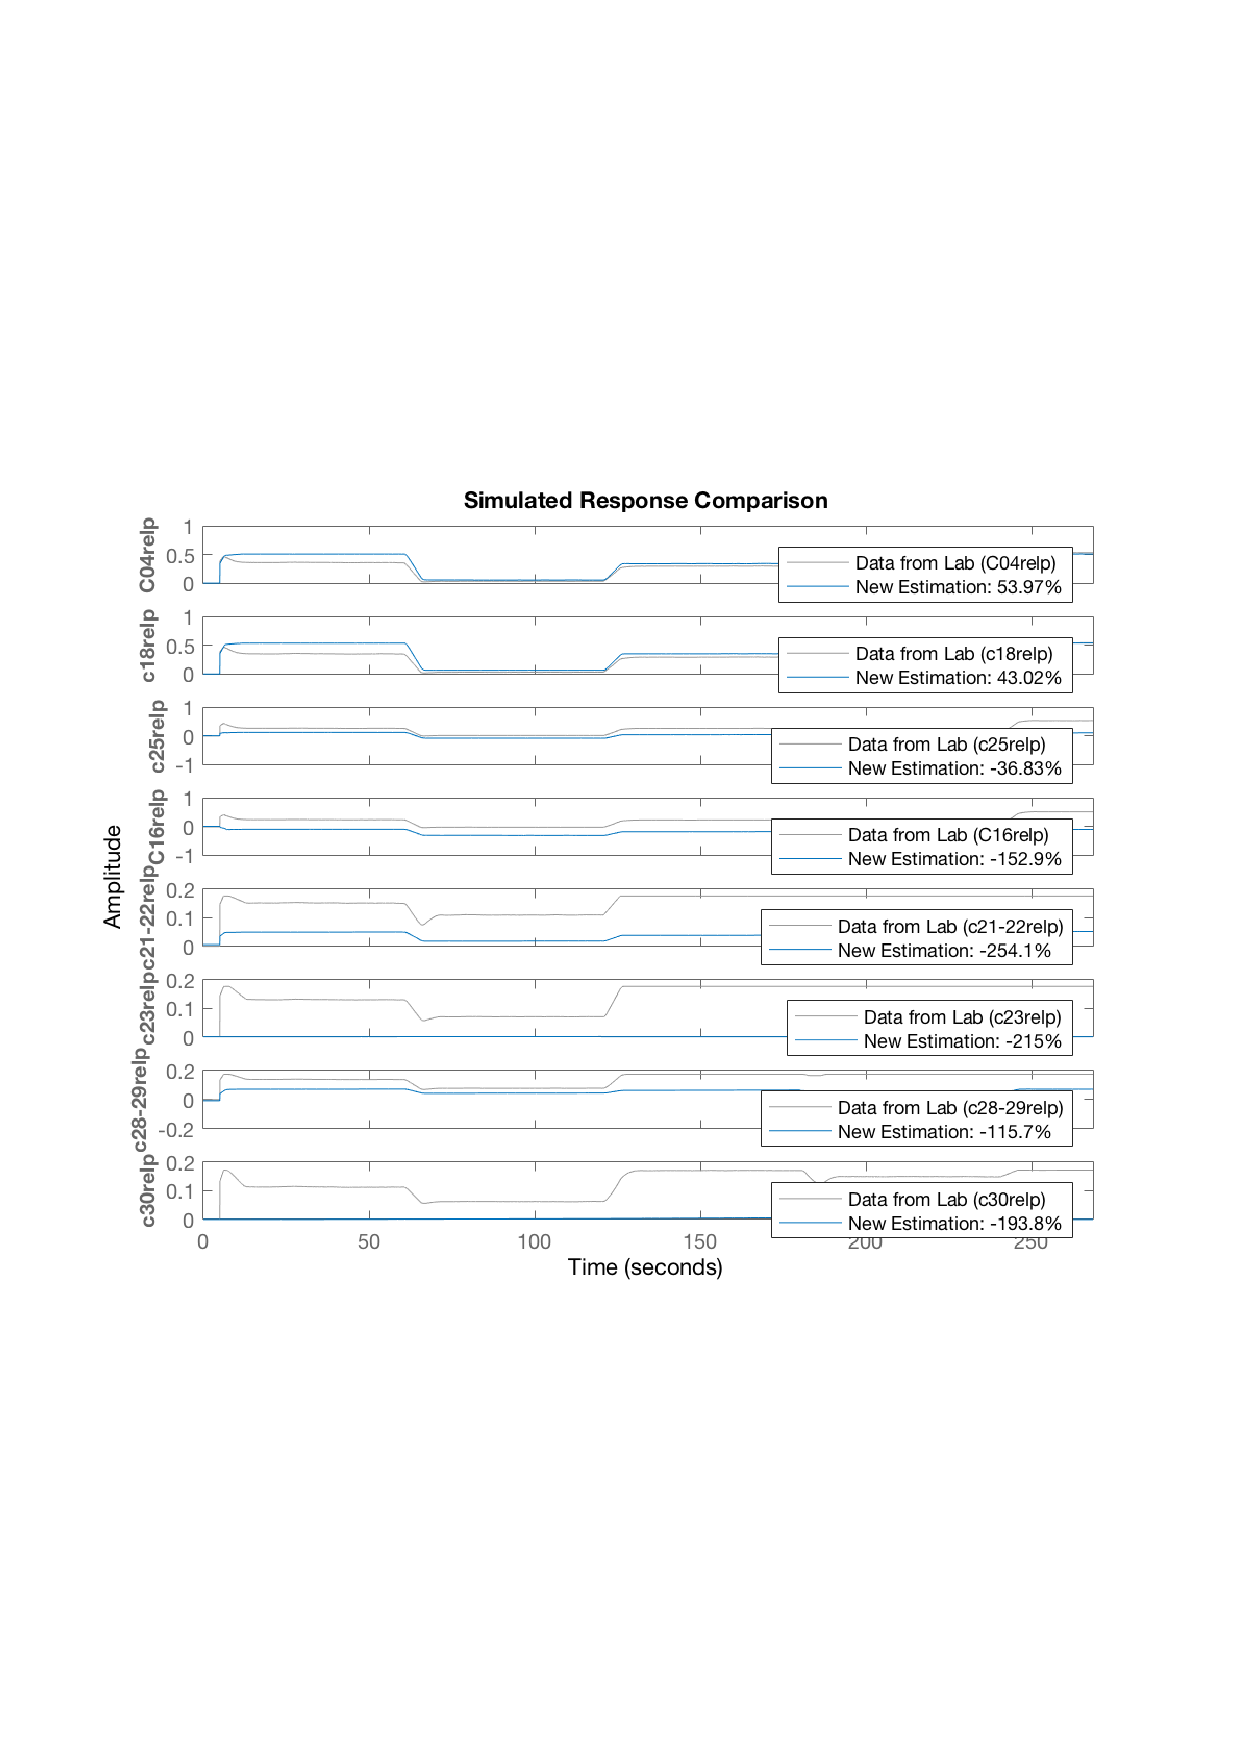
\includepdf[pages=-]{report/pictures/ComparePlot.pdf} 